%%%%%%%%%%%%%%%%%%%%%%%%%%%%%%%%%%%%%%%%%
% Oliver Lemon made minor edits (jan 2015)  to :
% Masters/Doctoral Thesis
% LaTeX Template
% Version 1.43 (17/5/14)
%
% This template has been downloaded from:
% http://www.LaTeXTemplates.com
%
% Original authors:
% Steven Gunn
% http://users.ecs.soton.ac.uk/srg/softwaretools/document/templates/
% and
% Sunil Patel
% http://www.sunilpatel.co.uk/thesis-template/
%
% License:
% CC BY-NC-SA 3.0 (http://creativecommons.org/licenses/by-nc-sa/3.0/)
%
% Note:
% Make sure to edit document variables in the Thesis.cls file
%
%%%%%%%%%%%%%%%%%%%%%%%%%%%%%%%%%%%%%%%%%

%----------------------------------------------------------------------------------------
%	PACKAGES AND OTHER DOCUMENT CONFIGURATIONS
%----------------------------------------------------------------------------------------

\documentclass[11pt, oneside]{Thesis} % The default font size and one-sided printing (no margin offsets)

\graphicspath{{Pictures/}} % Specifies the directory where pictures are stored

\usepackage{amsmath}
%\usepackage[square, comma, sort&compress]{natbib} % Use the natbib reference package - read up on this to edit the reference style; if you want text (e.g. Smith et al., 2012) for the in-text references (instead of numbers), remove 'numbers'
\hypersetup{urlcolor=blue, colorlinks=true} % Colors hyperlinks in blue - change to black if annoying

\title{\ttitle} % BUT you should use use " \title{\ttitle} " here instead to define the thesis title !
% \ttitle is defined in the file Thesis.cls

\hyphenation{pro-blem} % Fix hyphenation issues for some words

\begin{document}

\frontmatter % Use roman page numbering style (i, ii, iii, iv...) for the pre-content pages

\setstretch{1.3} % Line spacing of 1.3

% Define the page headers using the FancyHdr package and set up for one-sided printing
\fancyhead{} % Clears all page headers and footers
\rhead{\thepage} % Sets the right side header to show the page number
\lhead{} % Clears the left side page header

\pagestyle{fancy} % Finally, use the "fancy" page style to implement the FancyHdr headers

\newcommand{\HRule}{\rule{\linewidth}{0.5mm}} % New command to make the lines in the title page

% PDF meta-data
\hypersetup{pdftitle={\ttitle}}
\hypersetup{pdfsubject=\subjectname}
\hypersetup{pdfauthor=\authornames}
\hypersetup{pdfkeywords=\keywordnames}

%----------------------------------------------------------------------------------------
%	TITLE PAGE
%----------------------------------------------------------------------------------------

\begin{titlepage}
\begin{center}

\textsc{\LARGE \univname}\\[1.5cm] % University name
\textsc{\Large Masters Thesis}\\[0.5cm] % Thesis type

\HRule \\[0.4cm] % Horizontal line
{\huge \bfseries \ttitle}\\[0.4cm] % Thesis title
\HRule \\[1.5cm] % Horizontal line

\begin{minipage}{0.4\textwidth}
\begin{flushleft} \large
\emph{Author:}\\
\authornames
\end{flushleft}
\end{minipage}
\begin{minipage}{0.4\textwidth}
\begin{flushright} \large
\emph{Supervisors:} \\
\supname
\end{flushright}
\end{minipage}\\[3cm]

\large \textit{A thesis submitted in fulfilment of the requirements\\ for the degree of \degreename}\\[0.3cm] % University requirement text
\textit{in the}\\[0.4cm]
%\groupname\\

\deptname\\[2cm] % Research group name and department name

{\large \today}\\[1cm] % Date

\includegraphics[width=6cm]{./Figures/HWUlogo.jpg} % University/department logo - uncomment to place it

\vfill
\end{center}

\end{titlepage}

%----------------------------------------------------------------------------------------
%	DECLARATION PAGE
%	Your institution may give you a different text to place here
%----------------------------------------------------------------------------------------

\Declaration{

\addtocontents{toc}{\vspace{1em}} % Add a gap in the Contents, for aesthetics

I, \authornames, declare that this thesis titled, \guille{\ttitle} and the work presented in it is my own. I confirm that this work submitted for assessment is my own and is expressed in my own words. Any uses made within it of the works of other authors in any form (e.g., ideas, equations, figures, text, tables, programs) are properly acknowledged at any point of their use. A list of the references employed is included.

%\begin{itemize}
%\item[\tiny{$\blacksquare$}] This work was done wholly or mainly while in candidature for a research degree at this University.
%\item[\tiny{$\blacksquare$}] Where any part of this thesis has previously been submitted for a degree or any other qualification at %this University or any other institution, this has been clearly stated.
%\item[\tiny{$\blacksquare$}] Where I have consulted the published work of others, this is always clearly attributed.
%\item[\tiny{$\blacksquare$}] Where I have quoted from the work of others, the source is always given. With the exception of such %quotations, this thesis is entirely my own work.
%\item[\tiny{$\blacksquare$}] I have acknowledged all main sources of help.
%\item[\tiny{$\blacksquare$}] Where the thesis is based on work done by myself jointly with others, I have made clear exactly what %was done by others and what I have contributed myself.\\
%\end{itemize}
\vspace{2cm}
\textbf{Signed}: 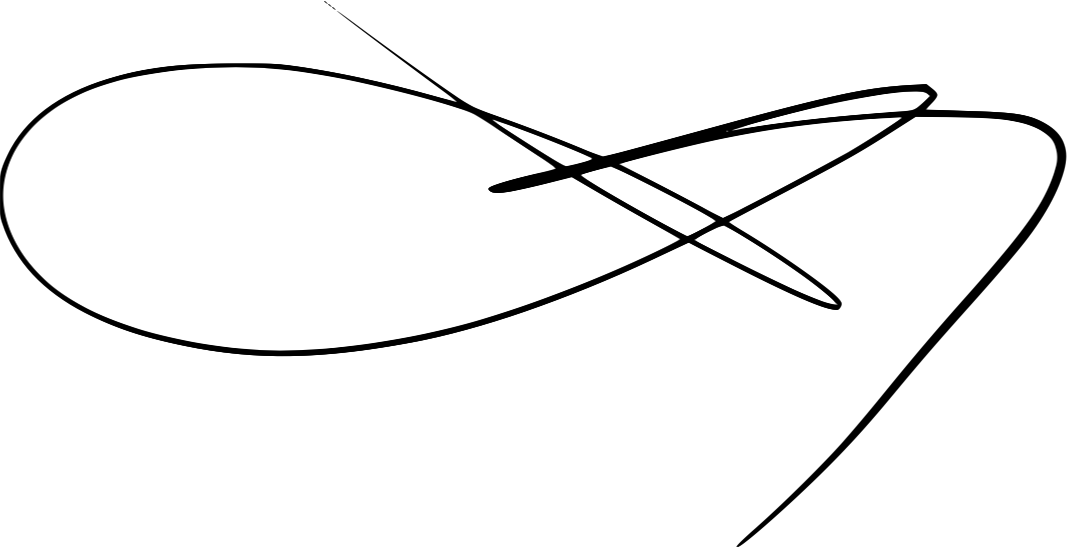
\includegraphics[width=5cm]{./Figures/Signature.png}\\
\rule[1em]{25em}{0.5pt} % This prints a line for the signature

\textbf{Date}: 24th of July, 2020 \\
\rule[1em]{25em}{0.5pt} % This prints a line to write the date
}

\clearpage % Start a new page

%----------------------------------------------------------------------------------------
%	ABSTRACT PAGE
%----------------------------------------------------------------------------------------

\addtotoc{Abstract} % Add the "Abstract" page entry to the Contents

%\abstract{\addtocontents{toc}{\vspace{1em}} % Add a gap in the Contents, for aesthetics

 {\huge{\textit{Abstract}} \par}{\addtocontents{toc}{\vspace{1em}}

Computers can represent numbers in different ways. Representations of them can differ in their binary translation. Integers, Floating-Point and Fixed-Point representations coexist with their own benefits and drawbacks. Reduced- and mixed- precision have been a focus of the literature since the 1960's. Using lower precision often increases performance at the cost of negligible loss in accuracy. The application are extremely diverse and growing emphasis is noticeable around machine learning and artificial intelligence. While training neural networks may require a powerful setup, deploying a network in an application should be possible on low-power, low-resource hardware architecture. Reconfigurable architectures have proven to be more powerful and flexible than GPUs when looking at a specific application. This thesis aims to assess the impact of mixed-precision when applied to a neural network deployed on reconfigurable hardware. While several frameworks have been developed to create tools to deploy neural network using reduced-precision, few benchmarks have been set up to assess the importance of quantisation and the quality of the benchmark. The benchmark set up here is used on top of \emph{FINN} and \emph{Brevitas}, two frameworks from Xilinx labs. While the results correspond to the intuition for neural networks using 2 to 16 bits for their parameters, networks using 32 bits precision seem to outperform the others both in terms of throughput and accuracy.
%The page is kept centered vertically so can expand into the blank space above the title too\ldots
%


\clearpage % Start a new page

%----------------------------------------------------------------------------------------
%	ACKNOWLEDGEMENTS
%----------------------------------------------------------------------------------------

\setstretch{1.3} % Reset the line-spacing to 1.3 for body text (if it has changed)

\acknowledgements{\addtocontents{toc}{\vspace{1em}} % Add a gap in the Contents, for aesthetics

My thanks go to every person that helped during the redaction of this paper. I am grateful for Pr. Loïc Lagadec and Dr. Pascal Cotret that proposed the subject to me. I thank them for their weekly guidance and help. I also want to express my gratitude for Pr. Rob Stewart that accepted to supervise the project as well. He helped ensure the report was resourceful and on point with the aimed project.

My thanks also go to the developers in the Xilinx Research Labs that guided me in a lot of steps through the development of their tools. My thanks go to M. Yaman Umuroglu, M. Alessandro Pappalardo and M. Henrik Borras for their insight and quality advice.
}
\clearpage % Start a new page

%----------------------------------------------------------------------------------------
%	LIST OF CONTENTS/FIGURES/TABLES PAGES
%----------------------------------------------------------------------------------------

\pagestyle{fancy} % The page style headers have been "empty" all this time, now use the "fancy" headers as defined before to bring them back

\lhead{\emph{Contents}} % Set the left side page header to "Contents"
\tableofcontents % Write out the Table of Contents

\lhead{\emph{List of Figures}} % Set the left side page header to "List of Figures"
\listoffigures % Write out the List of Figures

\lhead{\emph{List of Tables}} % Set the left side page header to "List of Tables"
\listoftables % Write out the List of Tables

\listof{mylisting}{List of code snippets}

%----------------------------------------------------------------------------------------
%	ABBREVIATIONS
%----------------------------------------------------------------------------------------

\clearpage % Start a new page

\setstretch{1.5} % Set the line spacing to 1.5, this makes the following tables easier to read

\lhead{\emph{Abbreviations}} % Set the left side page header to "Abbreviations"
\listofsymbols{ll} % Include a list of Abbreviations (a table of two columns)
{
\textbf{MNIST}    & \textbf{M}odified \textbf{N}ational \textbf{I}nstitute of \textbf{S}tandard and \textbf{T}echnology \\
\textbf{CIFAR-10} & \textbf{C}anadian \textbf{I}nstitute \textbf{F}or \textbf{A}dvanced \textbf{R}esearch 10            \\
\textbf{SVHN}     & \textbf{S}treet \textbf{V}iew \textbf{H}ouse \textbf{N}umbers                                       \\
\textbf{GTSRB}    & \textbf{G}erman \textbf{T}rafic \textbf{S}ign \textbf{R}ecognition \textbf{B}enchmark               \\

\textbf{FC Layer} & \textbf{F}ully-\textbf{C}onnected Layer                 \\
\textbf{NN}       & \textbf{N}eural \textbf{N}etwork                        \\
\textbf{CNN}      & \textbf{C}onvolutional \textbf{N}eural \textbf{N}etwork \\
\textbf{QNN}      & \textbf{Q}uantised \textbf{N}eural \textbf{N}etwork     \\
\textbf{BNN}      & \textbf{B}inarised \textbf{N}eural \textbf{N}etwork     \\

\textbf{GPU}      & \textbf{G}raphics \textbf{P}rocessing \textbf{U}nit                          \\
\textbf{CUDA}     & \textbf{C}ompute \textbf{U}nified \textbf{D}evice \textbf{A}rchitecture      \\
\textbf{MPI}      & \textbf{M}essage \textbf{P}assing \textbf{I}nterface                         \\
\textbf{NCCL}     & \textbf{N}vidia \textbf{C}ollective \textbf{C}ommunications \textbf{L}ibrary \\
\textbf{ASIC}     & \textbf{A}pplication \textbf{S}pecific \textbf{I}ntegrated \textbf{C}ircuit  \\

\textbf{FPGA}     & \textbf{F}ield \textbf{P}rogrammable \textbf{G}ate \textbf{A}rray \\
\textbf{HLS}      & \textbf{H}igh \textbf{L}evel \textbf{S}ynthesis                   \\
\textbf{LUT}      & \textbf{L}ook-\textbf{U}p \textbf{T}able                          \\
\textbf{FF}       & \textbf{F}lip-\textbf{F}lop                                       \\
\textbf{BRAM}     & \textbf{B}lock \textbf{R}andom \textbf{A}ccess \textbf{M}emory    \\
\textbf{DRAM}     & \textbf{D}ynamic \textbf{R}andom \textbf{A}ccess \textbf{M}emory  \\
\textbf{DSP}      & \textbf{D}igital \textbf{S}ignal \textbf{P}rocessor               \\

\textbf{I/O}      & \textbf{I}nput / \textbf{O}utput                       \\
\textbf{SVG}      & \textbf{S}tochastic \textbf{G}radient \textbf{D}escent \\
}

%----------------------------------------------------------------------------------------
%	THESIS CONTENT - CHAPTERS
%----------------------------------------------------------------------------------------

\mainmatter % Begin numeric (1,2,3...) page numbering

\pagestyle{fancy} % Return the page headers back to the "fancy" style

% Include the chapters of the thesis as separate files from the Chapters folder
% Uncomment the lines as you write the chapters

\chapter{Introduction}\label{chap_intro} % Main chapter title

\label{Chapter1} % For referencing this chapter elsewhere, use \ref{Chapter1}

\lhead{Chapter 1. \emph{Introduction}}

%----------------------------------------------------------------------------------------
%	SECTION 1.1 - Context
%----------------------------------------------------------------------------------------

\section{Context}

Ever since the creation of computers, their computation power has been a source of progress in terms of high-precision scientific computations in one hand or efficient energy expensive mass computations. In one case or the other, this performance has been met through the development of more and more performant hardware architectures. Moore forecasted the evolution through his law announced in 1965. However, the last decade has proven to counterbalance this law and makes it meet an end due to physical and thermal limitations. This decrease in hardware evolution has rather shifted the focus to other vectors of performance. One of them is parallelisation through the use of multiple or a cluster of computers. The goal is then to increase the computational power. This focus has enabled the development of new architectures tailored to those specific tasks, such as Graphical Processing Units (GPUs) or reprogrammable architectures such as Field Programmable Gate Arrays (FPGAs). In parallel, the use of reduced precision to increase the performance of computational-expensive tasks is a focus of the literature that can be applied particularly well to state-of-the-art hardware architectures. Next chapters look over the ideas under mixed-precision and the ways to implement them efficiently. Next derive applications that can benefit from the implementations and their translation to physical architectures.

%-----------------------------------
%	SECTION 1.2 - Aims and Objectives
%-----------------------------------
\section{Aims and Objectives}

The aim of the thesis is to give the reader an insight of the mixed-precision mindset and intentions by covering important articles and ideas the literature holds. The practical aim and result of the literature review is to implement a specific application using mixed-precision. This application consists of deploying a \emph{quantised neural network} (i.e. a neural network using reduced-precision) on a \emph{reconfigurable architecture}.

The resulting aims are the following. The objectives will be defined after the literature review in the \guille{Requirements analysis} chapter.

\textbf{Aims}
\begin{enumerate}
  \item Provide the reader with notions in \emph{Number Representation}.
  \item Provide the reader with notions in \emph{Machine Learning}.
  \item Provide the reader with notions in \emph{Hardware Architecture}.
  \item Link the three pools of notions through the \emph{Literature Review}.
  \item Present the objective of the project: Deploy a \emph{neural network} on a \emph{reconfigurable architecture}.
  \item Present the mixed-precision \emph{motivations} and \emph{implementation methods}.
  \item Present the mixed-precision \emph{applications} to machine learning.
  \item Present the \emph{frameworks} and \emph{deployment solutions} for machine learning on reconfigurable architectures.
  \item Present an \emph{implementation of a benchmark} over a framework.
  \item Display \emph{results of the benchmarking}.
  \item Provide the reader with \emph{critics} on the results.
  \item Give out possible \emph{future works} or applications.
\end{enumerate}

%-----------------------------------
%	SECTION 1.3 - Structure of the report
%-----------------------------------

\section{Structure of the report}

The given thesis is structured as follows. \textbf{Chapter 1} provides a brief \emph{Introduction} to the context and objectives of the report. \textbf{Chapter 2} consists of the \emph{Background}, presenting the main ideas behind both \emph{number representation}, \emph{machine learning} and \emph{hardware architectures}. \textbf{Chapter 3} covers the \emph{Literature Review} and how \emph{mixed-precision} was implemented and used, how it can be applied to \emph{neural networks} and how \emph{neural networks} can be deployed on specific architectures. \textbf{Chapter 4} consists of a \emph{Requirement Analysis} of the development project of the dissertation. \textbf{Chapter 5} presents any \emph{Professional, Legal, Ethical and Social Issues} the project can highlight. \textbf{Chapter 6} consists of a presentation of the implementation of the project, it goes over the main points and presents the tools and frameworks used as well as the experiments performed. \textbf{Chapter 7} presents the results of the experiments while \textbf{Chapter 8} discusses the results and leads to future works that can extend the project. Finally, \textbf{Chapter 9} is the \emph{Conclusion} of the thesis.

\chapter{Background} % Main chapter title

\label{Chapter2} % For referencing this chapter elsewhere, use \ref{Chapter2}

\lhead{Chapter 2. \emph{Background}}

%----------------------------------------------------------------------------------------
%	SECTION 2.1 - On Number representation
%----------------------------------------------------------------------------------------

\section{On Number Representation}

The question of the representation of numbers as we, humans, use them in a world of electronics has been central in the creation of computers and their associated arithmetics. Several problems are contained in the simple question of: How to translate our arithmetic and number operations in a piece of hardware?

%-----------------------------------
%	SUBSECTION 2.1.1 - Number Representation
%-----------------------------------
\subsection{Number Representation}

The first thing to note is that electronics can represent two states, a presence or absence of an electric impulsion. The states of \guille{on} and \guille{off} is embedded in transistors that can represent both. The transistor is the hardware representant of this duality while a bit is its software counter-part. This is the underlying reason why computers, even the first fully electronical computer ENIAC (\emph{Electronical Numerical Integrator and Computer}), use a binary system. If this system is handy to translate our base 10 arithmetic and simple numbers such as integers, it is harder to translate more complex numbers such as reals and floating point operations. The meaning of an N-bit binary word is entirely dependent of the interpretation we choose to use. This interpretation consists of both a representation (the type of the object the memory represents) and its associated mapping. Common number representations consists of unsigned integers, signed integers (using two's complement), floating point reals as well as fixed-point reals.

%-----------------------------------
%	SUBSUBSECTION 2.1.1.1 - Integer Representation
%-----------------------------------
\subsubsection{Integer Representation}

The representation of integers and especially unsigned integers is straightforward as it consists of a change form base 10 to base 2. This number representation can be done in 16-bits, 32-bits or 64-bits depending on its type, the supporting hardware and the space we need to contain it. Representing a number in base 2 from base 10 or vice versa is straightforward as it only demands simple and exact basic operations to be performed. As shown on \emph{Figure} \ref{fig:IntegerRepr}, $4576 = 2^5 + 2^6 + 2^7 + 2^8 + 2^{12}$.

Now, if we want to represent a signed integer, we have to use a method called the \emph{two's complement} in order to bring the sign in. This method keeps the basic behaviour of the addition to work on numbers be they positive or negative. The method consists in changing the value of all the bits of a given number then adding one to the result. The representation of -4576 when doing the computation with 13 bits (1 sign bit and 12 mantissa bits) consists of:
\begin{align}
(01000111100000)^\text{two's complement} &= (01000111100000)^\text{one's complement} + 1\\ \nonumber
                                         &= 10111000011111 + 1\\ \nonumber
                                         &= 10111000100000
\end{align}

The result for 32 and 64 bits can be seen on \emph{Figure} \ref{fig:IntegerRepr}.

\begin{figure}[htbp]
	\centering
		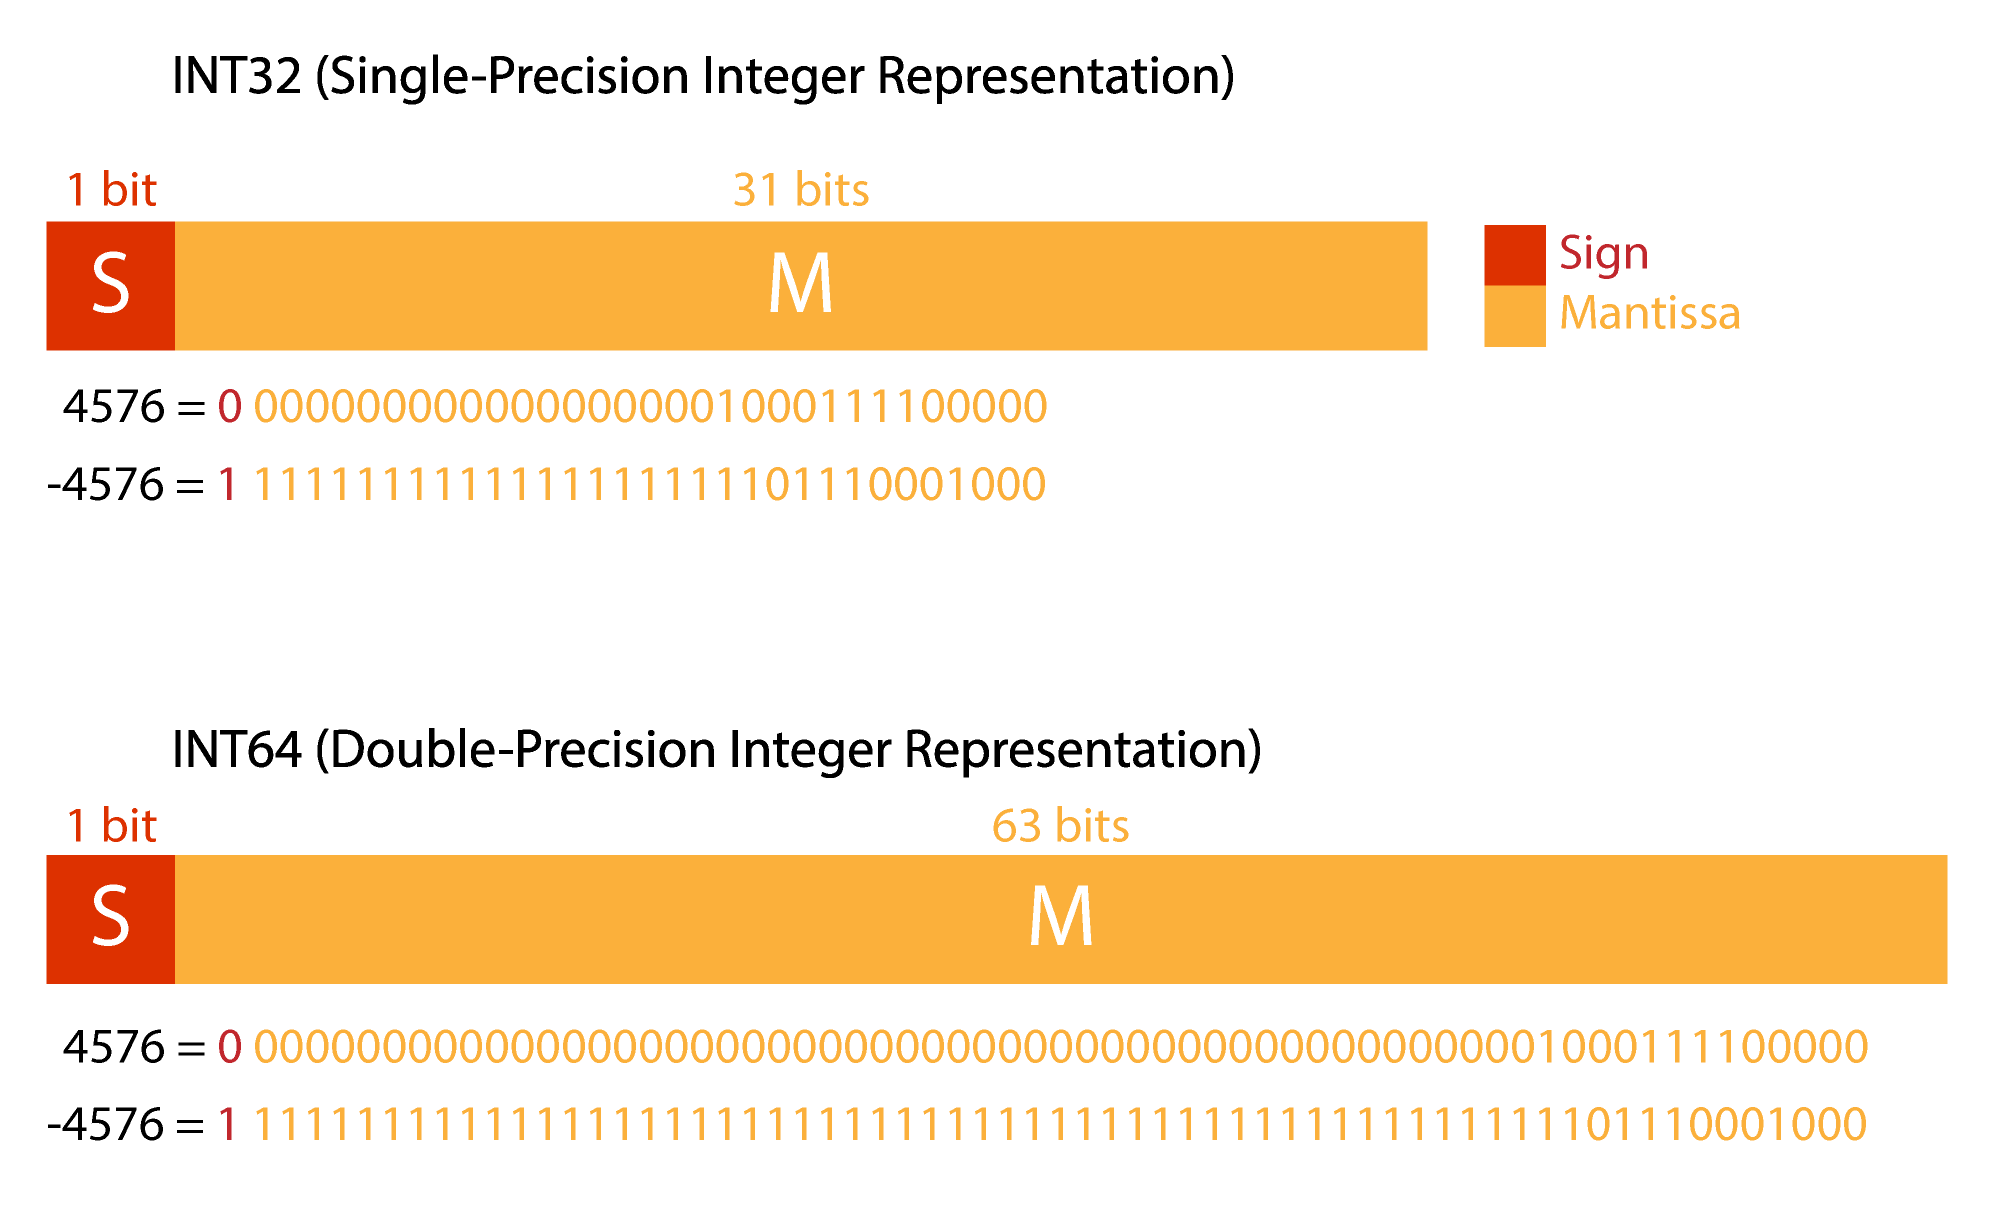
\includegraphics[width=.8\textwidth]{Figures/IntegerRepr.png}
	\caption[Integer Representation]{Integer Representation and Two's Complement example}
	\label{fig:IntegerRepr}
\end{figure}

% TODO CORRECT FIGURE

Those two representations allow a complete mapping of integers up to a certain range: signed 32-bit integers can represent numbers between -2,147,483,648 and 2,147,483,647 while unsigned integers can represent numbers between 0 and 4,294,967,295.

%-----------------------------------
%	SUBSUBSECTION 2.1.1.2 - Floating-Point Representation
%-----------------------------------
\subsubsection{Floating-Point Representation}

Representing floating-point numbers has been a concern since the 1980s and the industrial development of several computing modules and interfaces. The need for a consensus in this domain and particular applications has been answered by the IEEE-754 standard \cite{Ieee754_1985} in 1985. This standard defines both the floating-point number representations and exceptions conditions along with their default handling. This norm was reviewed fundamentally in 2008 \cite{Ieee754_2008}, extending it to 64-bits and 128-bits length. The last dated revision of the norm, at the time of writing, is from 2019 \cite{Ieee754_2019}.

Floating-point numbers following this representation are composed of three distinct elements:
\begin{enumerate}
  \item A sign bit
  \item An exponent
  \item A mantissa
\end{enumerate}

Those three elements compose the number by using the following formula: $(\mathit{sign}) \times \mathit{mantissa} \times 2^{\mathit{exponent}}$

In order to present both positive and negative exponents and as using the two's complement on the exponent would complexify the computation of floating-point numbers, a bias is used in the exponent. This bias corresponds to $2^e - 1$ where e is the number of bits of the exponent part. This means that with an 8-bit exponent, the bias is equal to 127. An exponent equal to $00000111$ is equal to $7 - 127 = -120$ and an exponent equal to $10000111$ is equal to $135 - 127 = 8$. An 8-bit exponent can cover a range from -126 to 127 (because exponents -127 (all 0s) and +128 (all 1s) are reserved for special numbers.

When referring to single-precision floating-point representation we are talking about 32-bit long memory representation. They are mapped as follows and as shown in \emph{Figure} \ref{fig:FP32}:
\begin{itemize}
  \item Sign bit: 1 bit
  \item Exponent: 8 bits
  \item Mantissa: 23 bits
  \item Exponent Bias: 127
\end{itemize}

% FP32 EXAMPLE
\begin{figure}[htbp]
	\centering
		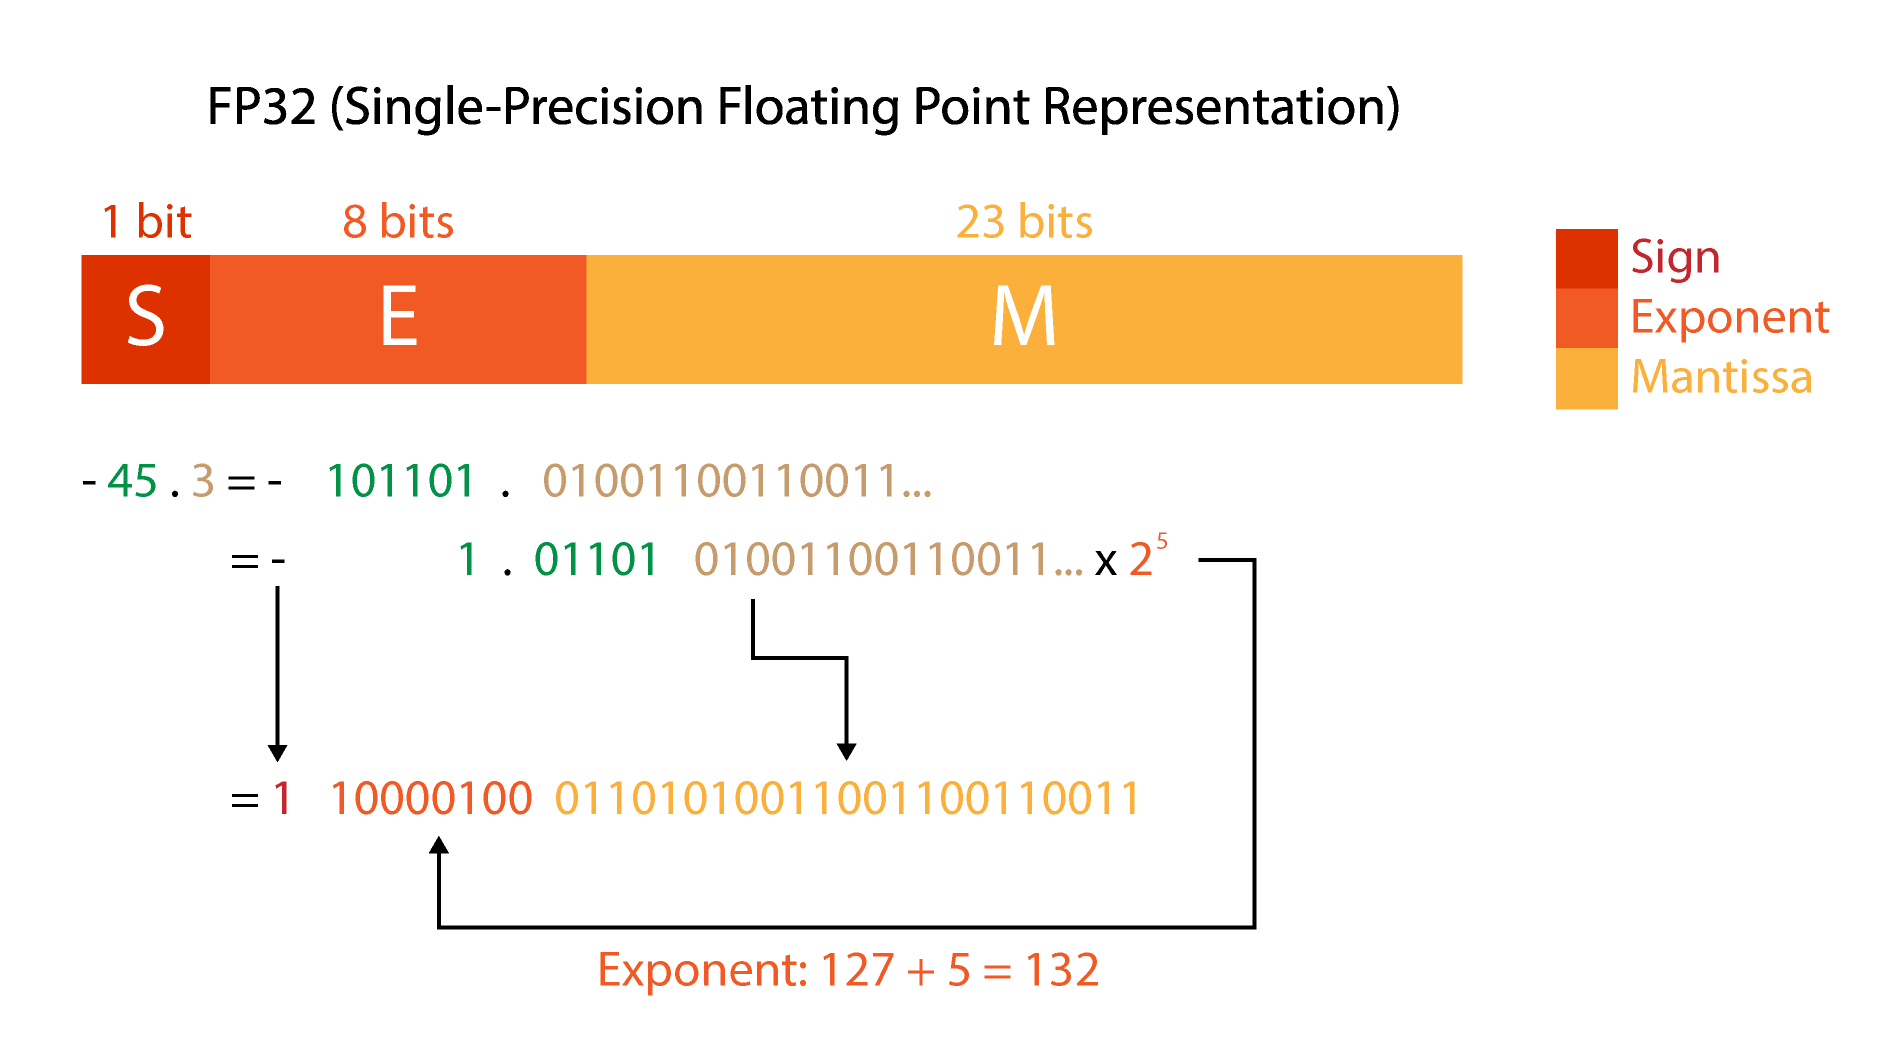
\includegraphics[width=.8\textwidth]{Figures/FP32.png}
	\caption[Single-precision float representation]{Example of the representation of a float in single-precision}
	\label{fig:FP32}
\end{figure}

% TODO CORRECT FIGURE

Referring to double precision floating-point representation means looking at 64-bit long memory representation, mapped as follows and as shown in \emph{Figure} \ref{fig:FP64}:
\begin{itemize}
  \item Sign bit: 1 bit
  \item Exponent: 11 bits
  \item Mantissa: 52 bits
  \item Exponent Bias: 127
\end{itemize}

% FP64 EXAMPLE
\begin{figure}[htbp]
	\centering
		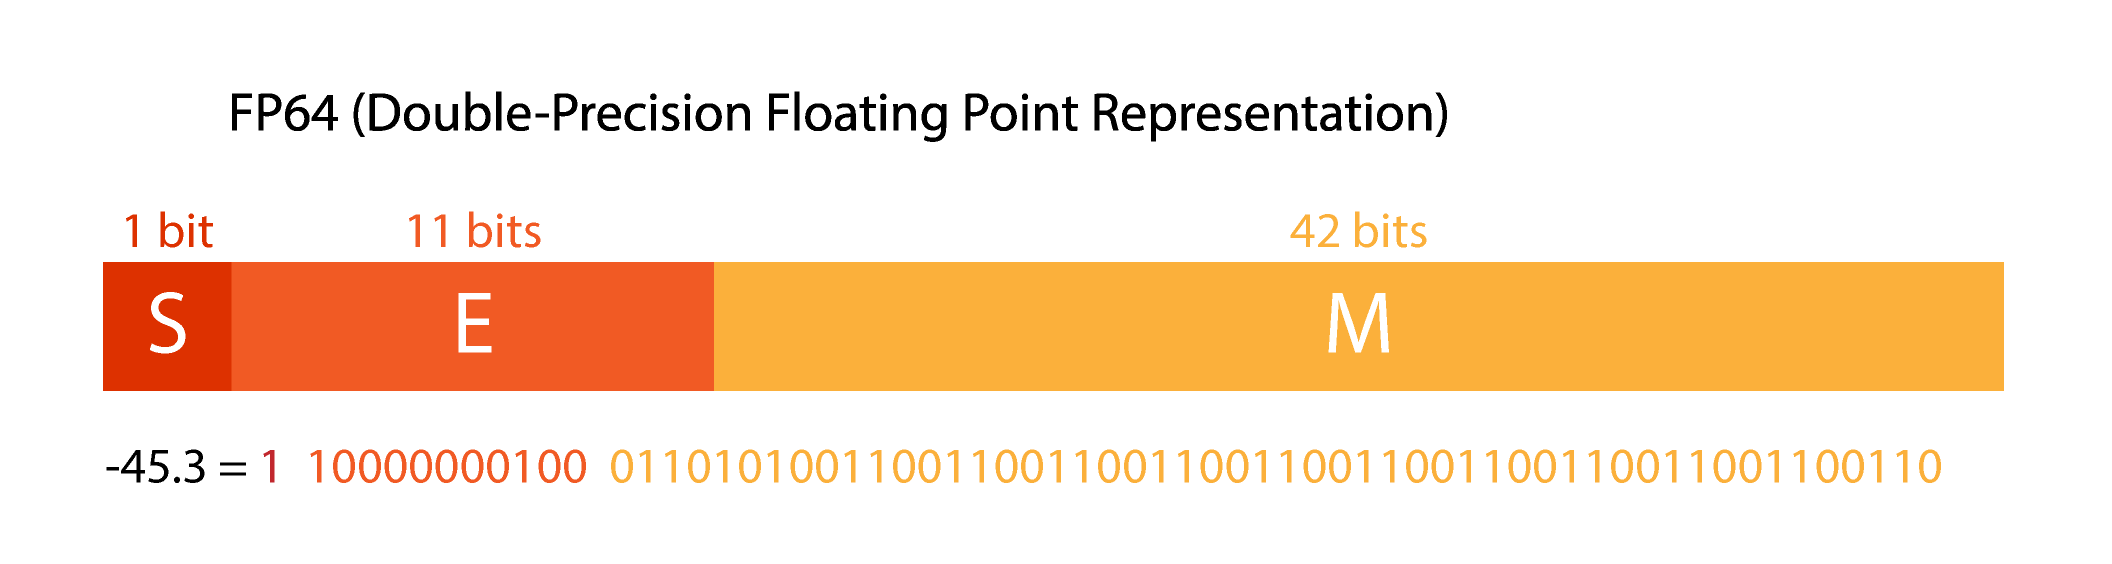
\includegraphics[width=.8\textwidth]{Figures/FP64.png}
	\caption[Double-precision float representation]{Example of the representation of a float in double-precision}
	\label{fig:FP64}
\end{figure}

% TODO CORRECT FIGURE

Along these representations, IEEE-754 introduces representations of special numbers. Positive and negative infinities are encoded with all 1s exponents and a fraction equal to zero. Zero is encoded with an all-0s exponent and fraction. Moreover, it adds methods to round floating-point numbers to positive or negative infinity, zero or to the nearest value.

%-----------------------------------
%	SUBSUBSECTION 2.1.1.3 - Fixed-Point Representation
%-----------------------------------
\subsubsection{Fixed-Point Representation}

Another way to look at the decimals is to fix the radix point to be at a certain place and keep it throughout all the computations and representations using this arithmetic. A fixed-point representation consists of three components:
\begin{enumerate}
  \item A sign indicator
  \item An integer corresponding to the total number of bits
  \item Another integer corresponding to the size of the fractional part
\end{enumerate}

Representing a number with this representation can be done by simply concatenating the base 2 representation of each side of the radix point. This means the integer part will be represented with positive powers of two ($2^0$, $2^1$, $2^2$$\ldots$) while the fractional part is represented with negative powers of two ($2^{-1}$, $2^{-2}$\ldots).

% FIXED POINT EXAMPLE
\begin{figure}[htbp]
	\centering
		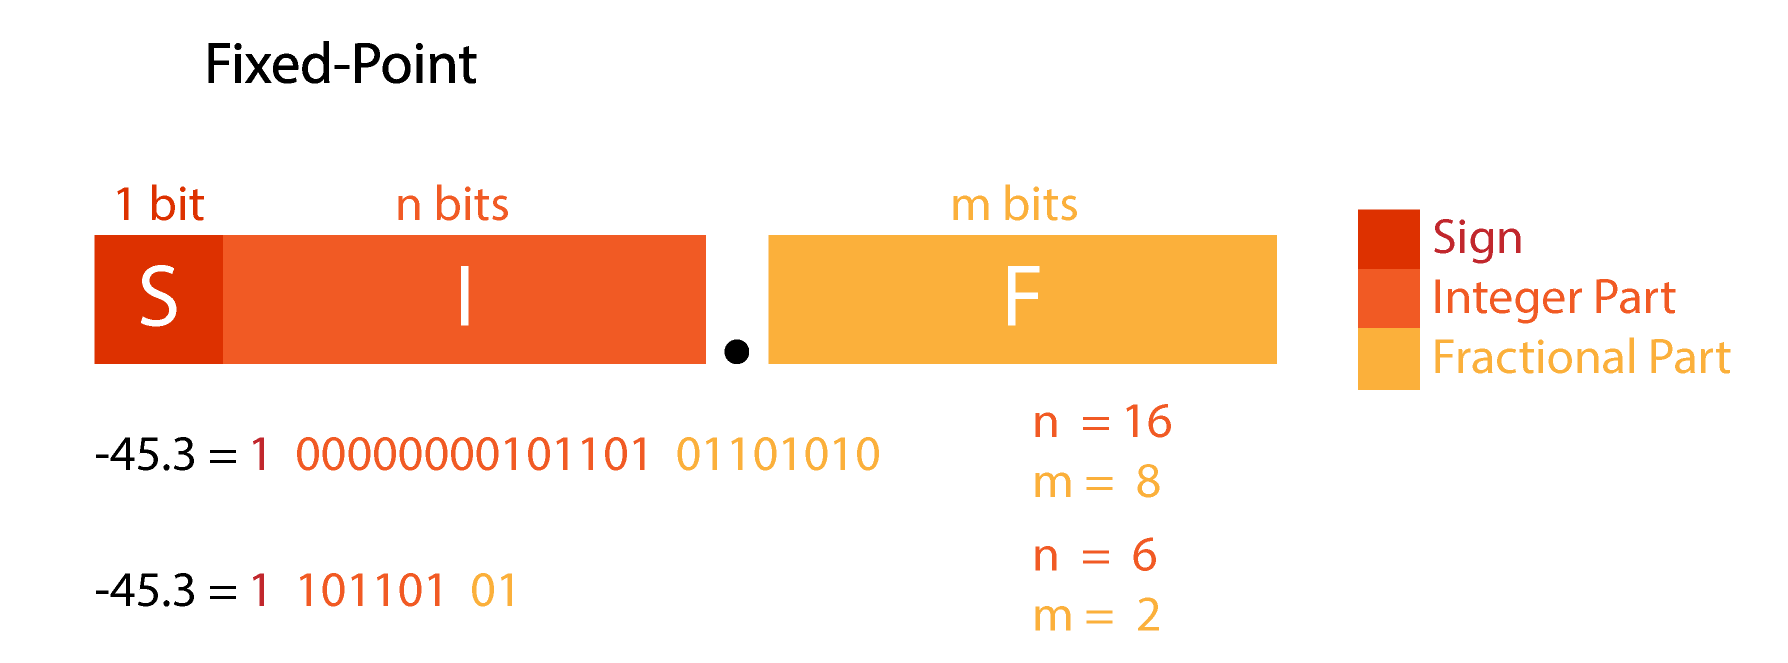
\includegraphics[width=.8\textwidth]{Figures/FixedPoint.png}
	\caption[Fixed-Point Representation]{Example of a float in fixed-point representation}
	\label{fig:FixedPoint}
\end{figure}

As shown in \emph{Figure} \ref{fig:FixedPoint}, several representations can depict the same decimal number. Finding the correct amount of bits to allocate to each side of the radix point is what will qualify the representation. Allocating fewer bits than needed may lead to overflow while allocating too much may increase quantisation errors.
Along with this new representation comes a whole new arithmetic. While this format can help tailor your needs in terms of variable types, it comes with an additional cost. The operations performed in this arithmetic are non-trivial as addition and multiplication are not associative and distributive anymore. This means the order of the operations will have an impact on the final result. Moreover, the round-off error underlying this representation is often non-trivial to grasp. However, those operations are low demanding in terms of computing power.

%-----------------------------------
%	SUBSECTION 2.1.2 - Performance Benchmarks
%-----------------------------------
\subsection{Metrics \& Performance benchmarks}

Floating-point representation (in either single or double precision) allows extreme precision at the cost of performance trade-offs (space or memory). On the other hand, fixed-point representation, even if it comes with a more complex arithmetic and insidious round-off errors, allows to tailor the type to your needs. Storing the values of the size and mass of planets in floating-point precision, would end up not using the majority of the range of values you selected while one could tailor a correct type in fixed-point representation.

The benchmarks in this field use several metrics in order to quantify and qualify the representations and their implementations.
\begin{itemize}
	\item \textbf{Size}: The size of a number in a given representation.
	\item \textbf{Energy cost}: The cost of operations in a given representation. \emph{The lower the better}.
	\item \textbf{Frequency}: The clock rate of a piece of hardware, or the quickness of pulses generation. \emph{The lower the better}.
	\item \textbf{Latency}: The access time of a piece of hardware to memory or external devices. \emph{The lower the better}.
	\item \textbf{Accuracy}: The precision enabled by a given representation. \emph{The higher the better}.
	\item \textbf{Memory Usage}: The memory needed to store both numbers and results of operations between them. \emph{The lower the better}.
	\item \textbf{Performance}: The overall time needed to complete a sequence of operations.
\end{itemize}

The operations performed in floating-point are expensive in terms of bandwidth, memory and energy consumption, which ultimately translate in to additional cost to perform an action. Horowitz's talk at ISSCC 2014 \cite{Horowitz2014} entitled \guille{Computing's Energy Problem (and what we can do about it)} provides an insight of the problems and challenges technology scaling has encountered in its development. Moore's law is getting outdated and a solution to the issue of permanently growing energy needs resides in \guille{the design of applications and hardware that are better matched to task and each other}. The numbers presented by M.Horrowitz have been reused by Professor William Dally (Standford University, NVidia Corporation) in his lecture on \guille{High-Performance Hardware for Machine Learning} \cite{Nips2015}. The \emph{Figure} \ref{fig:OpCosts} is extracted from this lecture and presents the energy and area costs different floating-point operations demand. Increasing precision on the used numbers increases the relative energy cost at the same time. An 8-bit addition costs 0.03 pJ whereas the same addition in 32-bit floating-point costs 0.9 pJ or 30 times more.

% COSTS OF OPERATIONS 2015-NIPS
\begin{figure}[htbp]
	\centering
		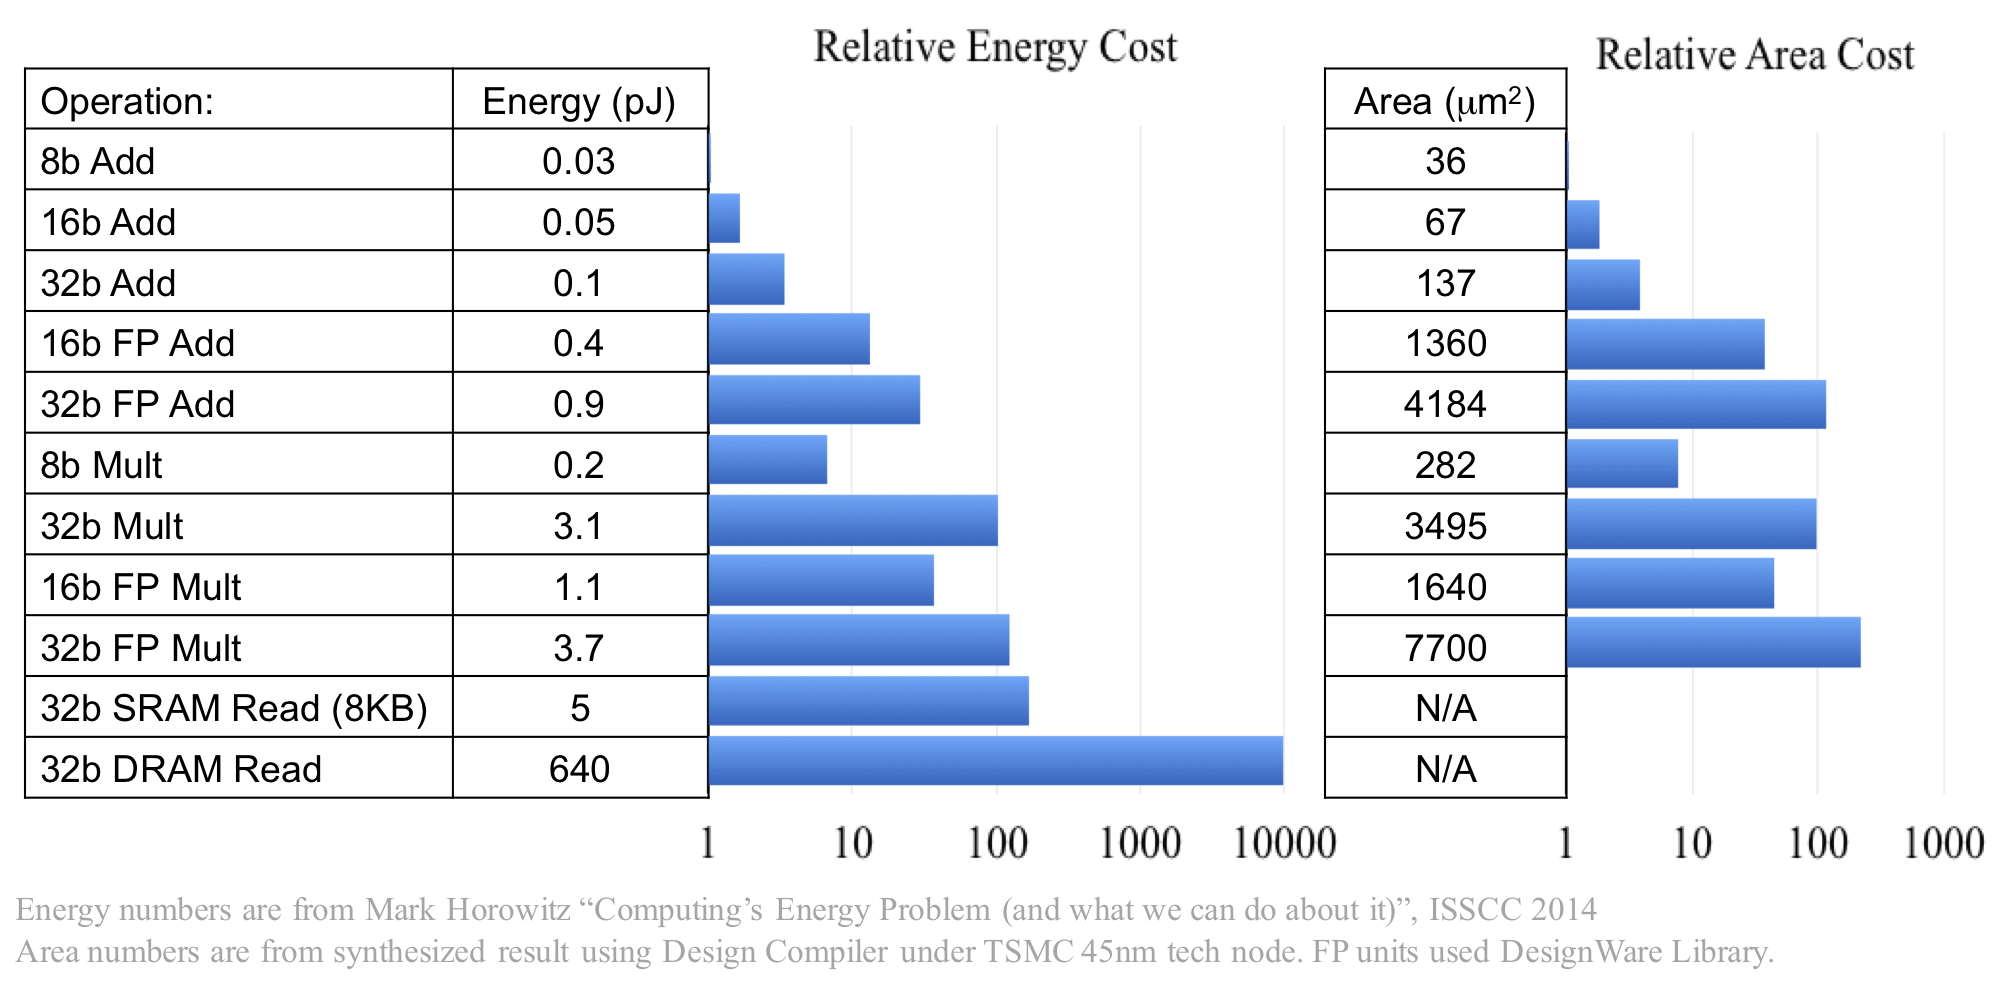
\includegraphics[width=\textwidth]{Figures/OpCosts.png}
	\caption[Operation costs]{Cost of operations in certain representations \cite{Nips2015,Horowitz2014}}
	\label{fig:OpCosts}
\end{figure}

The benefit of using a more optimised representation other the floating-point representation has been investigated as soon as in 2000 in \cite{Tong2000}. The authors present a way to reduce the energy consumption by minimising the bitwidth representation of the floating-point data. The data used to tailor the type representation is human-sensory data such as speech or video imagery. This kind of data is obtained at low precision (4 to 10 bits) but mapped into a full single-precision floating-point type. Using such optimisations, the authors manage to obtain a reduction of 66\% in multiplier energy per operation without sacrificing any accuracy.

Modifications of the representations can be embedded in the architecture. Xilinx, a manufacturer of state-of-the-art architecture, produced a white paper written by Finnerty et al. \cite{Xilinx2017} showing that their tools are able to handle fixed-point types and arithmetic and that the benefits are important:
\begin{itemize}
  \item Reduced power consumption
  \item Reduced use of resources (look-up tables, memory)
  \item Latency improvements
  \item Comparable performance and accuracy
\end{itemize}
The authors show the example of an FIR filter implementation in fixed-point representation from floating-point. The frequency is shown to be 16\% faster and the latency 7.5 times lower.

In conclusion, customising type in an environment where costs are translated in terms of energy consumption, memory or bandwidth usage, will always come out as an improvement. This redirects the issue to a need to guarantee little to no loss in accuracy.

%----------------------------------------------------------------------------------------
%	SECTION 2.2 - On Machine Learning
%----------------------------------------------------------------------------------------

\section{On Machine Learning}

Machine Learning is one of the most promising asset of the recent years since it has proven to be reliable when tackling complex issues. Those tasks can either be recognizing a street sign, a disease in a radiography or classifying a piece of text under a sentiment. Text-to-speech, speech-to-text, image classification, object detection, etc: those are all the domains machine learning is suited for. This section will provide insight on the basic functions machine learning uses, present neural network architectures and development frameworks.

%-----------------------------------------------
%	SUBSECTION 2.2.1 - Neurons and Neural Networks
%-----------------------------------------------

\subsection{Neural Networks}

 Machine learning has been extended to the use of neural networks. Karpathy et al. \cite{Karpathy2015} present the different structures in their lecture materials. The apparition of neural networks in machine learning comes from the analogy with the human brain and the way neurons work and communicate between each other. The analogy can be seen on \emph{Figure} \ref{fig:Neuron}.

% NEURON PRESENTATION
\begin{figure}[htbp]
	\centering
		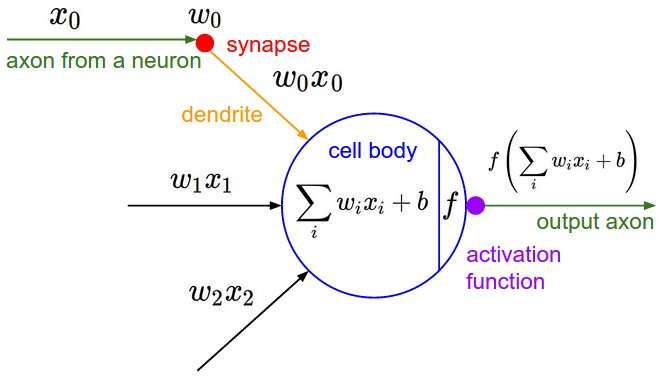
\includegraphics[width=8cm]{Figures/Neuron.png}
	\caption[Neuron Example]{Example of a neuron and its behavior in a neural network \cite{Karpathy2015}}
	\label{fig:Neuron}
\end{figure}

Each neuron receives several inputs from other previous neurons and performs an operation on all the received inputs to create the output that will go to its successors. A family of neurons that will obtain the outputs of the same neurons is called a \emph{layer}. A combination of \emph{layers} composes a \emph{neural network} as presented on \emph{Figure} \ref{fig:NN}.

% NEURAL NETWORK PRESENTATION
\begin{figure}[htbp]
	\centering
		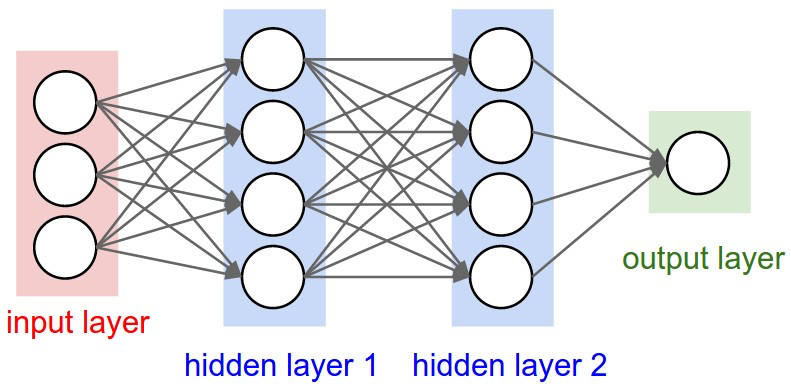
\includegraphics[width=8cm]{Figures/NN.png}
	\caption[Neural Network Example]{Example of a neural network architecture \cite{Karpathy2015}}
	\label{fig:NN}
\end{figure}

The neuron performs a simple dot product of all the inputs along with their weights, adds a bias to the sum and applies a given non-linear activation function. The weight will give importance to some of the inputs while hiding others. Throughout the training, some of the inputs will be shown to be more useful than others and their weight will be changed accordingly. The function used by the neuron (dot-product here) depends on the type of the layer the neuron is part of. The activation function models the \guille{firing rate of the neuron which [$\ldots$] represents the frequency of the spikes along the axoms}. It is often a simple non-linear function that will help a network have an answer against non-linear problems. The XOR function for example can be learned by a network composed of as little as two layers. Several choices of non-linear functions can be made for your neurons:
\begin{itemize}
  \item Sigmoid function: $\sigma(x) = \frac{1}{(1+e^{-x})}$
  \item Tanh: $tanh(x) = 2\sigma(2x) - 1$
  \item Rectified Linear Unit (ReLU): $ f(x) = max(0,x) $
\end{itemize}

Neural networks perform the simple operations of reducing the inputs, adding a bias and passing it through a non-linear function. However, it is possible to set up several layers where the first one is called the \emph{input layer}, the last one the \emph{output layer} and all the layers in-between the \emph{hidden layers}. These layers go one after each other as shown in \emph{Figure} \ref{fig:NN}. While having hidden neurons is useful to better comprehend the data fed to the network, having too much of them can lead to overfitting, including noise and outliers into the pattern recognition.

% TODO ADD FIGURE FOR FORWARD PROP BACK PROP AND

A neural network \guille{learns} by tuning its parameters. The tuning occurs in two phases: a \emph{forward} and \emph{backward} propagation. The \emph{forward} propagation consists of running an instance through the whole network. The \emph{backward} propagation defines a cost function that will measure how good the neural network performs. This cost can be obtained for an instance and the corresponding output the network. The network adjusts the parameters by using partial differentiates on the cost function. This cost is determined by the \emph{loss function}. Another important piece of the workflow is the optimiser. If the \emph{loss function} can determine how wrong the predictions are, the optimiser is the actual function modifying the parameters. It can adopt different strategies, the most well-known being \emph{Gradient Descent}. The \guille{amount of change} the optimiser is able to add depends on a hyper-parameter, the \emph{learning rate}.

Neural networks perform well in machine learning, but the fields where the architecture is mostly used are image and speech recognition. An extension of neural networks is used when the data is known to be of a certain type. For example, if the data is known to be images, Convolutional Neural Networks (CNN) are the best choice as they are tailored with the goal of handling images. They are a special type of neural networks in the sense that they use 3D layers and transformations on images. This choice of 3D layers comes from the fact that images are usually encoded in three channels, RGB (Red, Green and Blue). CNNs can be used for image classification, object detection, image segmentation or speech recognition. We will focus on image recognition here as this field provides well-known metrics and network layouts due to the popularity of the ImageNet Project for example \cite{ImageNet2009}. This popularity has attracted literature focus and allows comparisons and benchmarks to be made.

% NEURAL NETWORK PRESENTATION
\begin{figure}[htbp]
	\centering
		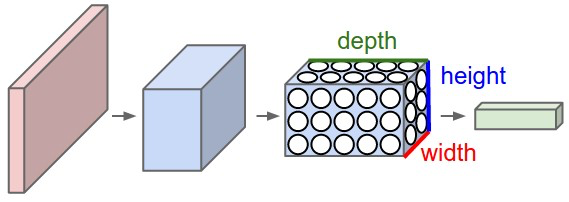
\includegraphics[width=8cm]{Figures/CNN.png}
	\caption[Convolutional Neural Network Example]{Example of a convolutional neural network architecture \cite{Karpathy2015}}
	\label{fig:CNN}
\end{figure}

Several layers are used and allow to perform different operations on images. The most used and well-known are the following:
\begin{itemize}
  \item Convolution   (CONV): Connects small regions of the input image through a filter. \emph{This layer helps extracting features such as edges or shapes.}
  \item Activation     (ACT): Apply an activation function (such as $max(0,x)$). \emph{This layer brings non-linearity into place.}
  \item Pooling       (POOL): Downsampling operation through a filter. \emph{This layer replaces a region of the image with the max or average value. It helps reducing noise.}
  \item Fully-Connected (FC): Computation of the class scores. \emph{This layer consists of a reduce operation and allows to compute the class scores.}
\end{itemize}

Layers take as input a set of data, known as a \emph{Feature Map} and output a new set of feature maps with higher-level semantics. Those layers then compose a CNN architecture and can be trained on a bank of images to adjust the different bias and weights for each layers and their corresponding neurons. Finally, once the network is trained, it can deduce the class of a given image. Those two steps are called \emph{Training} and \emph{Inference}, the training will work on a set of annotated data samples to create a model \guille{which semantics extrapolate outside the training set, [with a] \emph{modelling power}} \cite{Abdelouahab2018}. Once this step is completed, the \emph{Inference} phase can start and the network will have to classify new data instances. The training phase is extremely consuming in terms of time, energy and hardware resources. However, it only needs to be performed once. On the other hand, the inference has to be run each time a new instance is provided to the system. Therefore, if literature focus on accelerating both phases, an emphasis is put on inference as it will be needed to embed trained networks in lighter architectures.

%-------------------------------------------------
%	SUBSECTION 2.2.2 - Tools for Classification
%-------------------------------------------------

\subsection{Tools for Classification}

%-----------------------------------------------
%	SUBSUBSECTION 2.2.2.1 - Network Architectures
%-----------------------------------------------

\subsubsection{Network Architectures}

While there exists a wide range of applications for neural networks and machine learning in general, the field of image classification is the most suitable to benchmarking. Literature presents a wide and evergrowing number of neural networks, often backed up by reknowned companies. Historically, Yann Le Cun et al. \cite{LeCun1998} presented the first version of a CNN tailored to a specific task: recognizing handwritten digits. By the same occasion, they created the MNIST (Modified National Institute of Standards and Technology) dataset to benchmark their network architecture. All CNN architectures are composed of two main phases:
\begin{itemize}
  \item \emph{Feature Extraction}: This phase consists of an extraction of features by downsampling the image through several filter layers (convolutions, pooling but also batch normalisation and dropout).
  \item \emph{Classification}: This phase consists of flattening the output of the first phase and running it through several linear layers with varying number of neurons. The final linear layer will always have a number of neurons equal to the number of classes in the classification challenge.
\end{itemize}

The following figures are taken from Raimi Karim work for \emph{Towards Data Science} in \cite{Karim2020}.

Le Cun et al. \cite{LeCun1998} architecture chose to tackle the two phases by designing a neural network architecture called \emph{LeNet}. This architecture represents the feature extraction phase by using a succession of two $5 \times 5$ convolutions and $2 \times 2$ average pooling layers. Then, three linear layers (fully connected) perform the classification. Their respective size are 120, 84 and 10 (the number of classes in MNIST \cite{LeCun2010} case which it was designed for). The activation function used is hyperbolic tangent. This whole architecture is displayed on \emph{Figure} \ref{fig:LeNet-5} representing the version \emph{LeNet-5}.

% LeNet-5 PRESENTATION
\begin{figure}[htbp]
	\centering
		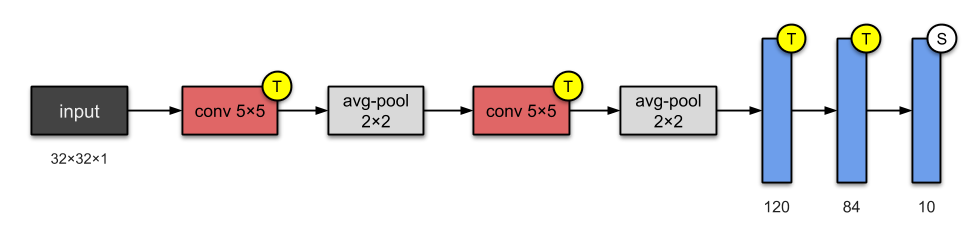
\includegraphics[width=10cm]{Figures/LeNet-5.png}
	\caption[LeNet-5]{Architecture of LeNet-5 as taken from \cite{LeCun1998}}
	\label{fig:LeNet-5}
\end{figure}

Krizhevsky et al. present \emph{AlexNet} \cite{Krizhevsky2012} in 2012, 14 years later, as the succesor of \emph{LeNet}. \emph{AlexNet} consists of deeper and wider version of \emph{LeNet}. There are now five convolution layers (of respective filter size $11 \times 11$, $5 \times 5$ and $3 \times 3$ for the remaining). Maximum pooling is used instead of average and it is the first time the ReLU function is used as an activation function ($max(0,x)$ as a reminder). The three final layers are now sized as 4096, 4096 and 1000 (the number of classes of the ImageNet \cite{ImageNet2009} dataset). This whole architecture is displayed on \emph{Figure} \ref{fig:AlexNet}.

% AlexNet PRESENTATION
\begin{figure}[htbp]
	\centering
		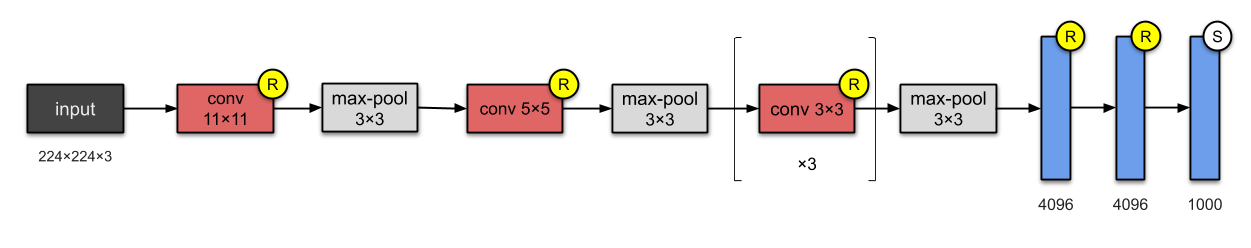
\includegraphics[width=12cm]{Figures/AlexNet.png}
	\caption[AlexNet]{Architecture of AlexNet as taken from \cite{Krizhevsky2012}}
	\label{fig:AlexNet}
\end{figure}


Using the same idea that Krizhevsky et al. \cite{Krizhevsky2012} had in mind when designing \emph{AlexNet} in 2014, Simonyan et al. took it a step further when designing \emph{VGGNet} \cite{Simonyan2014}. The VGG net comes with different versions (11, 13, 16 and 19) corresponding to the number of convolutions and fully-connected layers. Using only $3 \times 3$ convolution filters and the same size of linear layers, VGG-16 performed very well on ImageNet \cite{ImageNet2009}. Its architecture is displayed on \emph{Figure} \ref{fig:VGG-16}. One of the downside of this very-deep neural network is that it holds an enormous amount of parameters taking memory space. VGG-16 for example takes about 500MB of memory.

% VGG-16 PRESENTATION
\begin{figure}[htbp]
	\centering
		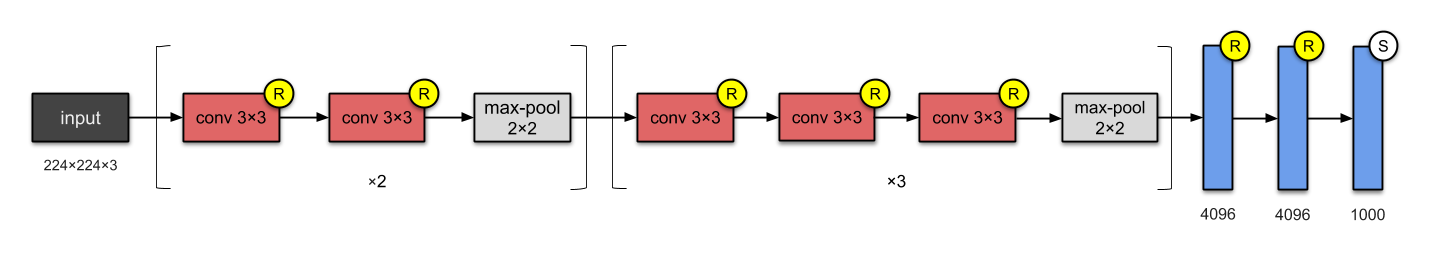
\includegraphics[width=14cm]{Figures/VGG-16.png}
	\caption[VGG-16]{Architecture of VGG-16 as taken from \cite{Simonyan2014}}
	\label{fig:VGG-16}
\end{figure}

From now on, extending the layer size and network depth does not seem to give better results. Reknowned companies are now enrolling in the battle to the best accuracy on the ImageNet dataset \cite{ImageNet2009} and Microsoft presents its \emph{ResNet} \cite{He2015} in the 2015 competition. \emph{ResNet} uses a method to add a way to skip some connections. During the training of a network, all weights receive an update proportional to the gradient. If this gradient is very small, the change in weight can be minimal and the network can stop its training. Microsoft Research used those skipping connections to conserve the signal and mitigate data loss. In other words, \emph{ResNet} breaks a deep neural network into smaller networks connected through skip or shortcut connections. Its architecture is displayed on \emph{Figure} \ref{fig:ResNet-50}.

% ResNet-50 PRESENTATION
\begin{figure}[htbp]
	\centering
		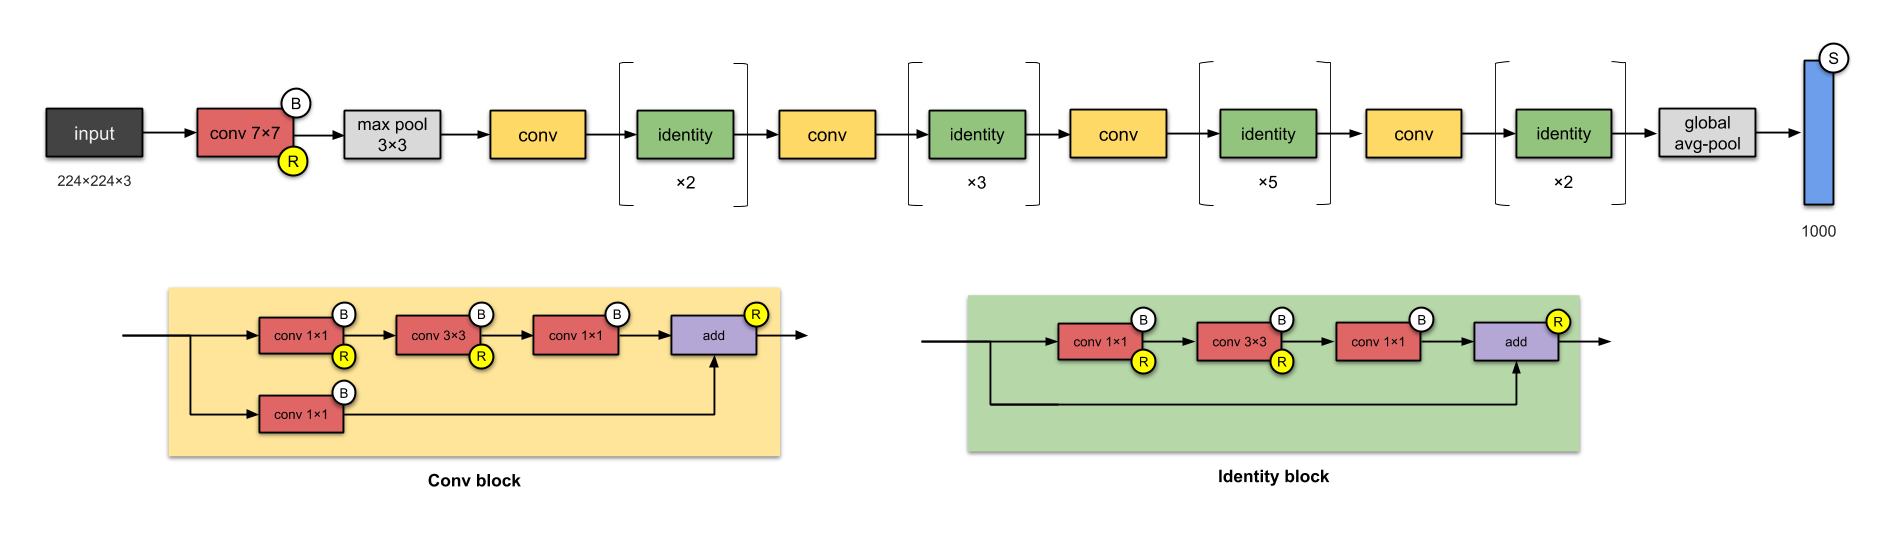
\includegraphics[width=15cm]{Figures/ResNet-50.png}
	\caption[ResNet-50]{Architecture of ResNet-50 as taken from \cite{He2015}}
	\label{fig:ResNet-50}
\end{figure}

Google came into place by proposing the \emph{MobileNet} \cite{Howard2017} architecture. This architecture, as its name shows, aims at being implemented in many mobile or light hardware architectures. Its emphasis is put on the size of the network and should allow the developer to tailor it to the needs of his aimed hardware architecture. The number of parameters is reduced by using a \guille{\emph{separable depthwise convolution}} that separates the usual $3 \times 3$ convolution into two parts. The first one applies the filter on the inputs and the second (a $1 \times 1$ filter called \guille{\emph{pointwise convolution}}) combine the outputs. Overall, this technique allows to reduce the number of parameters and operations while keeping state-of-the-art.

% % MobileNet PRESENTATION
% \begin{figure}[htbp]
% 	\centering
% 		\includegraphics[width=8cm]{Figures/MobileNet.png}
% 	\caption[MobileNet]{Architecture of MobileNet as taken from \cite{He2015}}
% 	\label{fig:MobileNet}
% \end{figure}

Many other networks exist and are still being developed actively. New techniques (e.g. batch normalisation \cite{Ioffe2015}) are getting incorporated in state-of-the-art architectures to get an even better result out of them. This list is in no way exhaustive but presents the milestones and wishes to translate the mindset operating in the machine learning community.

\emph{Table} \ref{tab:CNNTable} summarizes the different network architectures. It provides both the network name, year, paper it has been extracted from as well as its number of parameters. Moreover, the \emph{top-1} accuracy of the network on the ImageNet \cite{ImageNet2009} dataset is provided. We can see, as said earlier, that extending the network number of parameters has been the focus of state-of-the-art architectures until 2014. Next, the

\begin{table}[!]
  \centering
  \begin{tabular}{ | c c | c | c | c | }
    \hline
    \multicolumn{2}{|c|}{\textbf{Architecture}}  & \textbf{Year} & \textbf{Number of Parameters} & \textbf{Top-1 Accuracy} \\ \hline
    \textbf{LeNet}       & \cite{LeCun1998}      &     1998      &         0.6 M                 &           X             \\ \hline
    \textbf{AlexNet}     & \cite{Krizhevsky2012} &     2012      &          60 M                 &         63.3\%          \\ \hline
    \textbf{VGGNet (16)} & \cite{Simonyan2014}   &     2014      &         138 M                 &         74.4\%          \\ \hline
    \textbf{ResNet (50)} & \cite{He2015}         &     2015      &          26 M                 &         81.2\%          \\ \hline
    \textbf{MobileNet}   & \cite{Howard2017}     &     2017      &         4.2 M                 &         72.56\%         \\ \hline
  \end{tabular}
\caption[CNNTable]{Convolutional Neural Network Architectures}
\label{tab:CNNTable}
\end{table}

%----------------------------------
%	SUBSUBSECTION 2.2.2.2 - Datasets
%----------------------------------

\subsubsection{Datasets}
Architectures presented earlier are well-known and are still getting better with version iterations and the discovery of new techniques (batch normalisation, depth-wise convolution, residuals, etc.). On the other side, datasets have evolved to present each time a new and harder challenge for different architectures to perform on. Well-known datasets consist of the following:
\begin{itemize}
  \item \emph{MNIST} is the historical dataset, considered as the machine learning version of a classic \guille{\emph{hello world}}. It was implemented along with the \emph{LeNet} architecture and has been the default first dataset to train a network architecture on ever since. Several extensions to this dataset have been created since the dataset is juged to be \guille{too easy} to be a challenge to modern neuron architectures. Very simple CNN can achieve less than 3\% error on this dataset. Several drop-in replacements have been developed such as \emph{Fashion-MNIST} \cite{Xiao2017} - set up by Zalando with simple images of garnments -, \emph{Kuzushiji-MNIST} \cite{Clanuwat2018} - three versions on the recognition of Japanese characters - or even \emph{MNIST-MIX} \cite{Jiang2020} - a mix of handwritten digits from different languages -. All the instances of the MNIST dataset and its variations are images with only one channel (grey levels) and sized 28 pixels by 28 pixels. Those images are labelled in 10 different classes (digits from 0 to 9).

  % MNIST PRESENTATION
  \begin{figure}[htbp]
  	\centering
  		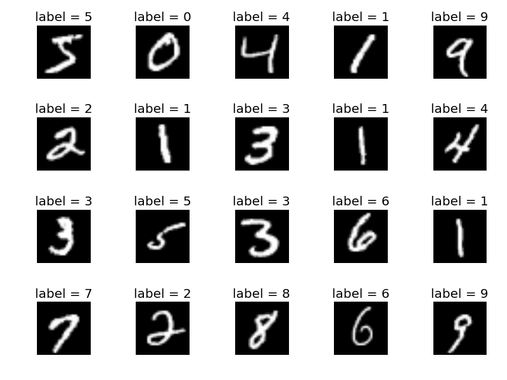
\includegraphics[width=8cm]{Figures/MNIST.png}
  	\caption[MNIST]{Instances extracted from the MNIST dataset}
  	\label{fig:MNIST}
  \end{figure}

  \item \emph{CIFAR-10} are labelled subset from the \emph{Tiny Images} dataset \cite{Krizhevsky2009}. It has been created in 2009 as collected and labeled automatically, supervised by three researchers from the MIT. This dataset is composed of tiny ($32 \times 32$) colored (3 channels) images of ten different classes: airplane, automobile, bird, cat, deer, dog, frog, horse, ship and truck. Instances taken from this dataset can be seen on \emph{Figure} \ref{fig:CIFAR-10} A more complicated dataset has been created in the same way. It is called \emph{CIFAR-100}, and as its name might suggest, contains a hundred different classes.

  % CIFAR-10 PRESENTATION
  \begin{figure}[htbp]
  	\centering
  		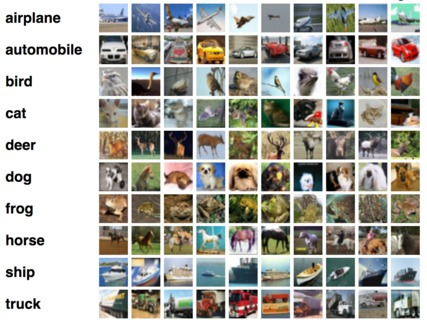
\includegraphics[width=8cm]{Figures/CIFAR-10.jpg}
  	\caption[CIFAR-10]{Instances extracted from the CIFAR-10 dataset}
  	\label{fig:CIFAR-10}
  \end{figure}

  \item With a growing emphasis put on autonomous vehicles, datasets have been developed accordingly. The two most well-known datasets covering this area are \emph{SVHN} (Street View House Numbers) \cite{Netzer2011} and \emph{GTSRB} (German Traffic Sign Recognition Benchmark) \cite{Stallkamp2012}. These two datasets have colored images of variable dimensions. \emph{SVHN} is an extension of \emph{MNIST} in the sense that it is a combination of different digits that the network will have to recognize. On the other hand, \emph{GTSRB} has been used in a 2012 competition and is useful to prototype self-driving components. \emph{GTSRB} contains 43 different classes of colored images and an instance of each of them can be seen on \emph{Figure} \ref{fig:GTSRB}.

  % % SVHN PRESENTATION
  % \begin{figure}[htbp]
  % 	\centering
  % 		\includegraphics[width=8cm]{Figures/SVHN.png}
  % 	\caption[SVHN]{Instances extracted from the SVHN dataset}
  % 	\label{fig:SVHN}
  % \end{figure}

  % GTSRB PRESENTATION
  \begin{figure}[htbp]
  	\centering
  		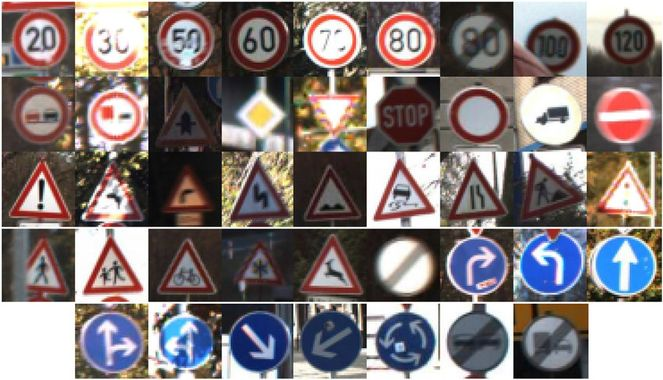
\includegraphics[width=8cm]{Figures/GTSRB.jpeg}
  	\caption[GTSRB]{Instances extracted from the GTSRB dataset}
  	\label{fig:GTSRB}
  \end{figure}

  \item Finally, \emph{ImageNet} \cite{ImageNet2009} is one of the largest dataset developed. It has been put up by a team from the Princeton University and is the centre of a challenge each year where state-of-the-art architectures confront themselves to get the best accuracy possible. The challenge is named the ImageNet Large Scale Visual Recognition Challenge (ILSVRC). Every year, contesters try to get the best possible accuracy out of the network they propose. The images contained in the dataset are $224 \times 224$ colored images split in 20,000 classes. The dataset contains more than 14 million images and has become the benchmark to determine the accuracy and robustness of state-of-the-art architectures.

  % IMAGENET PRESENTATION
  \begin{figure}[htbp]
  	\centering
  		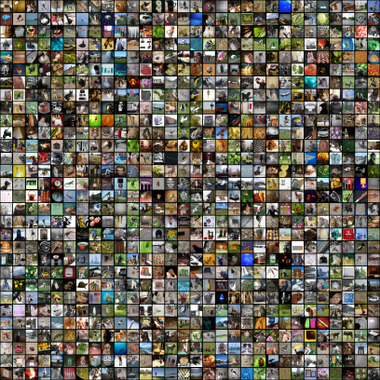
\includegraphics[width=8cm]{Figures/ImageNet.png}
  	\caption[ImageNet]{Instances extracted from the ImageNet dataset}
  	\label{fig:ImageNet}
  \end{figure}

\end{itemize}

% TODO: INCLUDE Table simplifying the different datasets

\begin{table}[!]
  \centering
  \resizebox{\textwidth}{!}{
  \begin{tabular}{ | c c | c | c | c | c | c | }
    \hline
    \multicolumn{2}{|c|}{\textbf{Name}}              & \textbf{Year} & \textbf{Channels} & \textbf{Image Size} & \textbf{Instances}  & \textbf{Number of Classes} \\ \hline
    \textbf{MNIST}           & \cite{LeCun1998}      &     1998      &  1 (Grayscale)    &   $28 \times 28$    &  60,000 / 10,000    &    10     \\ \hline
    \textbf{FashionMNIST}    & \cite{Xiao2017}       &     2017      &  1 (Grayscale)    &   $28 \times 28$    &  50,000 / 10,000    &    10     \\ \hline
    \textbf{Kuzushiji-MNIST} & \cite{Clanuwat2018}   &     2018      &  1 (Grayscale)    &   $28 \times 28$    &  60,000 / 10,000    &    10     \\ \hline
    \textbf{MNIST-MIX}       & \cite{Jiang2020}      &     2020      &  1 (Grayscale)    &   $28 \times 28$    & 397,440 / 99,360    &   100     \\ \hline
    \textbf{CIFAR-10}        & \cite{Krizhevsky2009} &     2009      &  3 (RGB)          &   $32 \times 32$    &  50,000 / 10,000    &    10     \\ \hline
    \textbf{CIFAR-100}       & \cite{Krizhevsky2009} &     2009      &  3 (RGB)          &   $32 \times 32$    &  50,000 / 10,000    &   100     \\ \hline
    \textbf{SVHN}            & \cite{Netzer2011}     &     2011      &  3 (RGB)          &   $32 \times 32$    &  73,260 / 26,000    &    10     \\ \hline
    \textbf{GTSRB}           & \cite{Stallkamp2012}  &     2012      &  3 (RGB)          &   $15 \times 15$ to $250 \times 250$      &    50,000 / 10,000   &    43     \\ \hline
    \textbf{ImageNet}        & \cite{ImageNet2009}   &     2009      &  3 (RGB)          &  $224 \times 224$   &   14M / 50,000      &  1000     \\ \hline
  \end{tabular}
  }
\caption[DatasetTable]{Datasets}
\label{tab:DatasetTable}
\end{table}

%-----------------------------------------------------
%	SUBSUBSECTION 2.2.2.3 - Development Frameworks
%-----------------------------------------------------

\subsubsection{Development Frameworks}

As research in the field of machine learning keeps growing and attracting more and more focus, many different development frameworks emerged to propose a high-level API and environment to experimental needs. Major industrial actors used this opportunity to present their own development API. Most of them have been under development for nearly a decade and still continue to attract a growing audience.

\begin{itemize}
  \item \emph{Tensorflow} has been the initiative of Google in 2011 and its source code has been opened in 2015. It is, to this day, the most used development framework in the field of machine learning. Its API is designed for Python and C++. However, due to increasing attention, numerous bindings to other languages have been created (Java, C\#, Haskell, etc.). Tensorflow set the milestones for AI frameworks by implementing production-ready resource distribution to deploy one's network to anyy architecture (CPU, GPU or a cluster). It also implements the idea of a \emph{tensor}, a ditributed array.
  \item Microsoft launched in 2015 its \emph{Cognitive Toolkit (CNTK)} written in C++ that aims at the same objectives as \emph{Tensorflow}: easy network creation through a high-level API and simplified deployment to a variety of architectures.
  \item The first version of \emph{Caffe (Convolutional Architecture for Fast Feature Embedding)} was developed in the University of Berkeley in 2014. In 2017, Facebook used \emph{Caffe} in an extended version called \emph{Caffe2} and as of May 2018, \emph{Caffe2} is officially merged in the \emph{PyTorch} project.
  \emph{Torch} is a Lua-based framework that was created in 2002. It is not in active development anymore since 2018 but \emph{PyTorch}, a Python implementation of the same underlying logic is in active development with a specific focus on the research community. \emph{Pytorch} aims at rapid prototyping and flexible architectures.
\end{itemize}

In the end, choosing a framework depends on one's objectives and knowledge of the language used. Benchmarks are getting released with, for example, Luo et al. \cite{Luo2020} that present a mobile implementation of several network architectures (\emph{ResNet, Inception, DenseNet, etc.}) implemented in \emph{TensorFlow Lite, Caffe2 and PyTorch Mobile}. The benchmark the authors propose is named \emph{AIoTBench} and focuses on computer vision.

% TODO: INCLUDE Table comparing the different development frameworks

%----------------------------------------------------------------------------------------
%	SECTION 2.3 - Hardware Architecture
%----------------------------------------------------------------------------------------

\section{On Hardware Architecture}

Moore's law \cite{Moore2006} predicted the evolution of hardware capacities in years to come when defined in 1965. It is an empirical relationship and in no means a physical or natural law but has shown to be exact for the thirty years following its creation. The Moore's law, when announced in 1965 said that \guille{the number of components per integrated circuit would double every year}. This law held for a decade and was then revised to \guille{doubling every two years} for the next decade. This law has been an industry guideline and helped produce long term business plans. However, the law is slowly coming to an end and has been shown to not fulfill the prophecy anymore due to physical limitations such as thermal restrictions. New architectures will have to take the lead as more computational power is still needed for the years to come. What are the new ways and architectures to increase performance even more?

%-----------------------------------
%	SUBSECTION 2.3.1 - GPU
%-----------------------------------

\subsection{GPU}

One solution to enable hardware acceleration is to parallelise computationally expensive tasks. GPUs (\emph{Graphics Processing Units}) are specialised electronic circuits that can handle computationally demanding tasks such as 3D rendering, video encoding and decoding or any action that can be massively parallelised (cryptocurrency digging, matrix computations or brute-force cracking). Few companies actually conceive and sell such systems. The most famous are NVidia, AMD and Intel and some smaller fabless - conceive the circuit but integrally subcontract the production -  companies such as Qualcomm or ARM. Other manufacturing companies such as ASUS or MSI will then integrate those circuits into products and calibrate them along with a cooling system that can make it enhance its base abilities.

Along with GPUs come their proper Software Development Kit (SDK) in order for developers to use their tools. NVidia invested heavily in CUDA (\emph{Compute Unified Device Architecture}) \cite{CUDA} and its aim is to reproduce a C syntax and environment for GPUs. AMD and Intel provide open-source SDK that tools then built upon.

GPUs allow computers to delegate expensive tasks (3D rendering for example) from the CPU to them. The GPUs can be either integrated or external. They require less knowledge than FPGAs but provide a more static architecture that will limit tuning opportunities. Mixed-precision mindset will not reach its full potential with this architecture but will still manage to increase the performance of different operations and tasks.

GPU provide an easy access to parallelisation and allow researchers of different fields to experiment with different precisions and parallelisation. One field that benefits a lot from it is the field of physics and applied simulations. Inherently, mathematics benefit a lot from reduced precisions in terms of computation times and resource utilisation to perform clasic operations such as matrix factorisation. Next are some examples of GPU application in the world of mixed-precision along with the hardware used.

\begin{itemize}
  \item \emph{Mathematics:} Haidar et al. \cite{Haidar2018} present a mixed-precision method to factorise a matrix into two triangular matrices. In order to perform their experiments, they use two 10-cores \emph{Intel Xeon e5-2650 v3} CPUs and one \emph{NVidia V100 PCLe} GPU.
  \item \emph{Mechanical Engineering:} Goddeke et al. \cite{Goddeke2007} present a survey paper on mixed-precision applied to \emph{Finite Element Simulations}, a widely used method in physics simulations that often require extensive computational resources. In their experiments, they use an \emph{AMD Athlon64 X2 4400} CPU and an \emph{NVidia GeForce 7800 GTX} GPU.
  \item \emph{Geosimulation:} Ichimura et al. \cite{Ichimura2018} present a mixed-precision earthquake simulator with an IA designed to help the solver converge. They use several super-computers such as the \emph{Summit} comprising two \emph{IBM Power9} processors and six \emph{NVidia Volta V100 accelerators}.
  \item \emph{Nuclear physics:} Clark et al. \cite{Clark2010} use mixed-precision in their work on simulating the quarks\' interactions in a nucleon. They use an \emph{NVidia GeForce GTX 280} GPU.
\end{itemize}

GPUs represent a fair part of the marketshare due to their various usages. They often come as a cheap and easy access to parallelisation since they have a wide and diverse community with ready-to-go frameworks and implementations.

%-----------------------------------
%	SUBSECTION 2.3.2 - FPGA
%-----------------------------------

\subsection{FPGA}

On the other hand, the 1990s have seen the birth of a new type of architecture: reconfigurable hardware. They allow to create application-specific hardware and are mixed-precision by default. Xilinx, one of the most famous FPGA manufacturer describes them as consisting of \guille{up to two million logic cells that can be configured to implement a variety of software algorithms} \cite{Xilinx2017}. Those logic cells can be dynamically reconfigured and this is the strength of this architecture.

Modern FPGAs contain components that are specialised for specific functions as well as more general purpose configurable logic. The combination of specific components with the configurable logic has allowed for architectures that consume less power and perform more efficiently.
\begin{itemize}
  \item \emph{Configurable Logic Block (CLB):} A \emph{CLB} is the most basic FPGA component which provide both logic and storage functionalities. It can be anything like a transistor, NAND gate, multiplexor or any combination of these. It often comes with a \emph{Look-Up Table (LUT)} to perform logic operations and a \emph{Flip-Flop (FF)} acting as a register for the results of the \emph{LUT}.
  \item \emph{Digital Signal Processing (DSP) Block:} A \emph{DSP block} is a specialised component of an FPGA that is designed to carry out \emph{digital signal processing} functions such as filtering or multiplying. It is designed to be much more efficient than if it was made with several \emph{CLBs}.
  \item \emph{Transceiver:} A \emph{trans-ceiver} is made to \emph{trans}-mit and re-\emph{ceive} serial data (individual bits) to and from the FPGA at extremely high rates. It also checks for erroneous data in the transmission. Having a dedicated component made it both quicker and easier to communicate with the FPGA.
  \item \emph{Block Random Access Memory (BRAM):} A \emph{BRAM} is the dedicated memory on the chip. This type of block can be divided or cascaded to make smaller or larger memory chunks available.
  \item \emph{Input/Output (I/O) Block}: The \emph{I/O block} operates, as its name gives out, as a component through which data transfers in and out of the FPGA. They are similar to \emph{transceivers} but are more flexible in functionality while operating at slower speed.
\end{itemize}

Along with those base components come many high-end more interesting components that can help develop the hardware to be tightly linked to the application one has in mind. As stated by \cite{Goddeke2007}, FPGAs have native mixed-precision processors and \guille{there is no need to utilise the same number format throughout the algorithm, or even the same operation}. Moreover, the freedom in the number representation can lead to alternative feasible number representations, such as a logarithmic one.

FPGAs can help prototyping chips and perform system validation, including pre-silicon validation, post-silicon validation and firmware development. Manufacturers can therefore validate their design before the chip is produced in factory. The end product can be an ASIC for example, an extremely powerful computing unit that is tailored to one function and one function only. Even though FPGAs are slower than ASICs and consume more power, their inherent ability to be reconfigurable makes them interesting in certain applications. Microsoft uses FPGAs to speed up Bing searches and still be able to change the search algorithm if needed. The efficiency versus flexibility can be seen on \emph{Figure} \ref{fig:EfficiencyVSFlexibility}.

% FPGA/ASIC comparison
\begin{figure}[htbp]
	\centering
		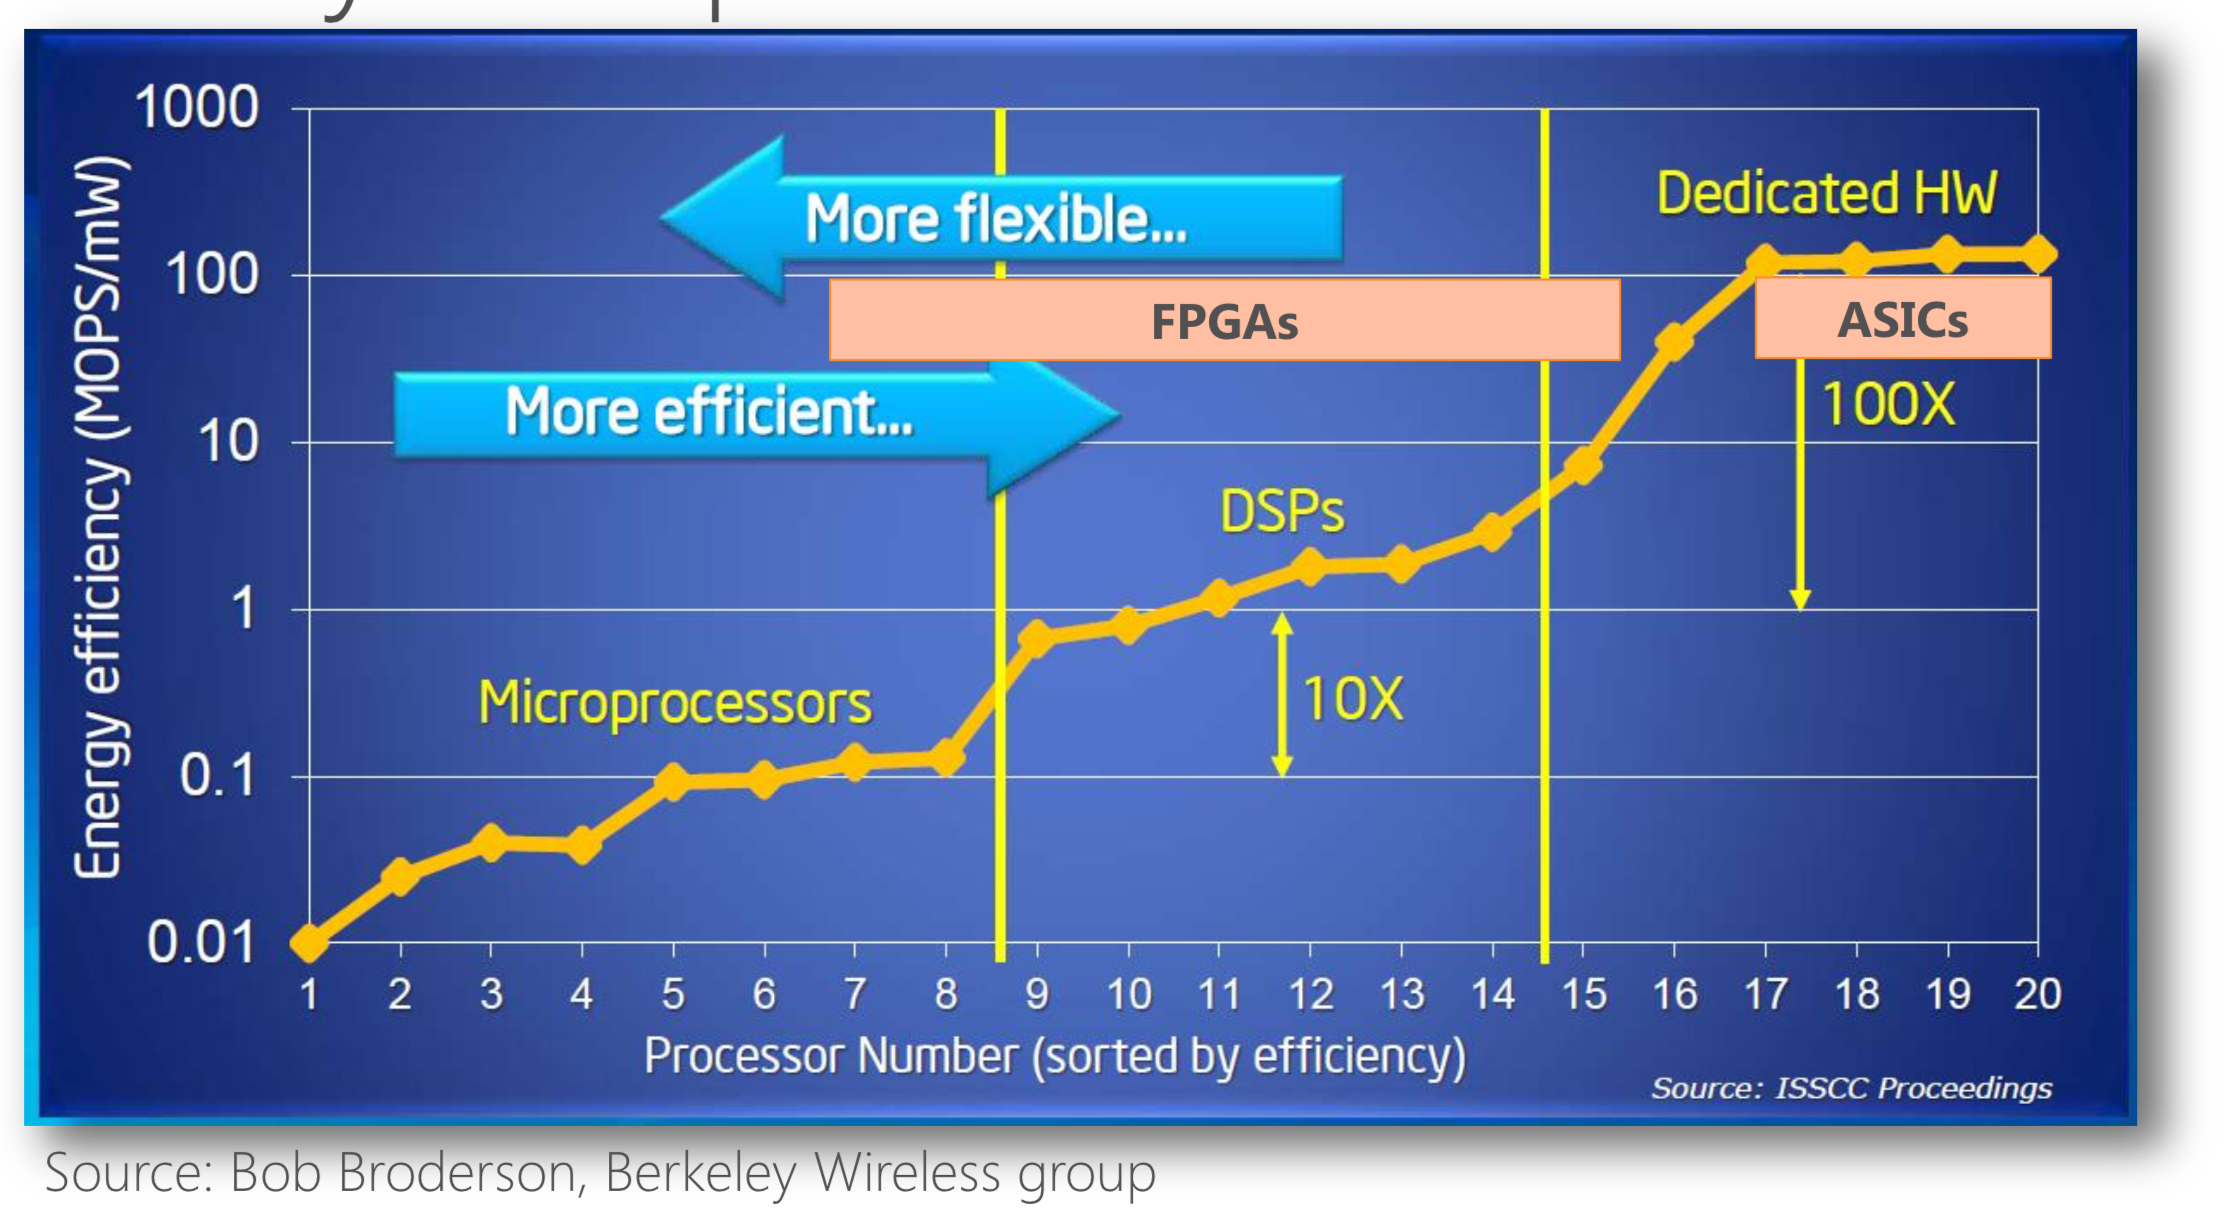
\includegraphics[width=10cm]{Figures/EfficiencyVSFlexibility.png}
	\caption[EfficiencyVSFlexibility]{Efficiency vs Flexibility}
	\label{fig:EfficiencyVSFlexibility}
\end{figure}

The whole development cycle shown in \emph{Figure} \ref{fig:FPGACycle} can be controlled using a high-level development language such as \emph{Xilinx Vivado} GUI or Smalltalk as in \cite{XuanSang2014}. In the end, programming an FPGA consists of testing a design all the way through the process (with testbenchs and simulations) while performing a synthesis of the different components and deploying the resulting \emph{bitfile} on the hardware architecture.

% FPGA Development Cycle
\begin{figure}[htbp]
	\centering
		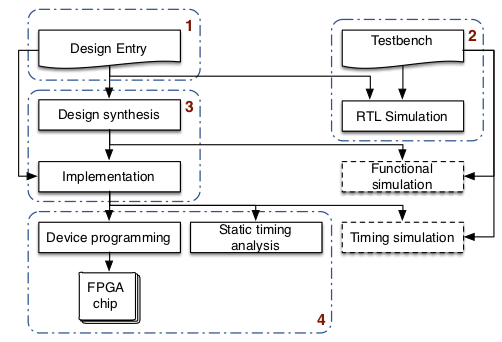
\includegraphics[width=10cm]{Figures/FPGACycle.png}
	\caption[FPGA Development Cycle]{FPGA Development Cycle \cite{XuanSang2014}}
	\label{fig:FPGACycle}
\end{figure}

\chapter{Literature Review} % Main chapter title

\label{Chapter3} % For referencing this chapter elsewhere, use \ref{Chapter2}

\lhead{Chapter 3. \emph{Literature Review}}

%----------------------------------------------------------------------------------------
%	SECTION 3.1 - Mixed Precision
%----------------------------------------------------------------------------------------

\section{Mixed Precision}

The first section explained in details the different existing number representations. With a particular emphasis on the representation of floating-point number, it has shown what the underlying issues of such representations are. The question now is how can we use to our advantage the different types along with their strengths and weaknesses?

%-----------------------------------
%	SUBSECTION 3.1.1 - Motivations
%-----------------------------------
\subsection{Motivations}

The term \guille{mixed precision} comes from the idea of using different precisions (type representations) to increase the performance of a computation that would otherwise only use the highest available (or user-defined) precision. The previous section showed us that each number representation has its pros and cons. Using lower precision types and representations will allow the total computation to decrease the usage of several hardware resources (memory, bandwidth, energy consumption) \cite{Horowitz2014,Nips2015}.

However, if lower-precision is acceptable, using mixed-precision can increase the capacity of smaller systems and subsystems as it will increase the overall performance and resources usage. This goal is targeted when you are aiming for the most performant processor, being given a size and type of usage. Moreover, this can be used when you know exactly the tasks your system will perform as well as their needed size. Yates \cite{Yates2007} presents several rules allowing  to determine the required size of any operation performed in fixed-point arithmetic. This arithmetic allows to tailor the type size to one's needs. Reconfigurable hardware can take advantage of this as well by using the exact required size for an operation. Such architecture will be looked upon in the next sections.

Scientific computations often require the highest available precision and the reduced precision induced by the lower-precision components is unacceptable. In order to still take advantage of the several gains lower-precision provides, a compromise has to be found about how and when to use lower-precision. Ideas on the usage have been looked upon since the 1950s and the first methods to correctly implement them in the early 1960s.

In any case, the developer has to know and keep in mind:
\begin{itemize}
  \item Required end precision
  \item Acceptable error rate
  \item Actual operations performed by the system
\end{itemize}

Mixed precision methods consist of doing a large part of the computation in low-precision components and only a small part in high-precision. As presented in the survey paper \cite{Goddeke2007} using different formats in the same algorithm can have several beneficial properties such as:
\begin{itemize}
  \item Accuracy: Same accuracy when up to 99\% of the operations is performed in the low format
  \item Computation: Low precision operations require less transistors and can translate in more paralellism
  \item Memory: Reduction in size in memory influences the efficiency and bandwidth requirements positively
\end{itemize}

%-----------------------------------
%	SUBSECTION 3.1.2 - Methods and Implementations
%-----------------------------------

\subsection{Methods and Implementations}
Several methods to actually implement a mixed precision algorithm have been developed starting 60 years ago. If the methods are different in practice, the theory behind them is the same as they aim to delegate most of the work to low-precision components while only using high-precision to recover the desired accuracy for the computation.

%-----------------------------------
%	SUBSUBSECTION 3.1.2.1 - Iterative Refinement
%-----------------------------------

\subsubsection{Iterative Refinement}

Since the early 1960s, literature has studied the effects and ways to implement mixed precision. The first reported works to implement such methods are James H. Wilkinson \cite{Wilkinson1994} and Cleve Moler \cite{Moler1967}. The method presented by both is named \guille{iterative refinement} and uses a combination of accumulative inner products along with a linear solver. This solution is directed towards the resolution of a system in the form of $Ax=b$ for a quadratic $N*N$ matrix $A$. The main idea is to use a residual between the wanted result and the result obtained by the last iteration. This residual is computed using high precision and accumulated using high-precision as well while the resolution of the equation is done in low-precision.

% Iterative Refinement Example
\begin{figure}[htbp]
	\centering
\begin{tabular}{ll}
	$x^{(0)}=0$ &\\
	$d^{(s)}=b-Ax^{(s)}$ & Compute residual in \emph{high} precision\\
	$Ac^{(s)}=d^{(s)}$ & Solve equation system in \emph{low} precision\\
	$x^{(s+1)}=x^{(s)}+c^{(s)}$ & Accumulate solution in \emph{high} precision\\
\end{tabular}
	\caption[Iterative Refinement]{Iterative Refinement Method \cite{Goddeke2007}}
	\label{fig:IterativeRef}
\end{figure}

This method has later been reused and extended. Baboulin et al. \cite{Baboulin2009} combine single- and double-precision floating-point numbers to enhance the performance of \guille{dense and sparse linear algebra algorithms}. Strzodka et al. \cite{Strzodka2006} present an enhanced algorithm to resolve a partial differential equation (Poisson problem) to present the effects of a mixed-precision approach. Sun et al. \cite{Sun2008} reproduce a linear solver in mixed-precision but adds an error analysis. The last two articles implement the result of their research on a reprogrammable architecture. Several applications profit directly from these papers and their implementations of mixed-precision algorithms as seen in later sections.

%-----------------------------------
%	SUBSUBSECTION 3.1.2.2 - Iterative Refinement
%-----------------------------------

\subsubsection{Analysis and Rewriting}

When creating a new application or system, any developer tends to use the highest available (or one of the highest) to represent the numbers he will need. However, the space and operations performed on higher-precision types are, as shown earlier, not the most performant. A simple, yet effective way to choose the correct type is to analyse the code and rewrite types that can be represented by lower precision ones. This idea has been implemented in the code analysis tool Precimonious \cite{Rubio2013} for floating-point representations. This analysis tool can go over the code and determines parts of it where lower precision can apply.

The mixed-precision approach can apply from a different perspective when using a fixed-precision representation. Darulova et al. \cite{Darulova2013} show that several polynomial expressions over the reals are cast over fixed-point arithmetic without being optimised, leading approximations of the real values. The tool they present allows to determine the best fixed-point implementation of a real number thanks to genetic programming. Then, as the order of operations is impactful when dealing with fixed-point arithmetic (distributivity and associativity are not respected), the tool reorder the operations to optimise the error and accuracy.

Those two tools have been brought together in \cite{Darulova2018} under the \guille{first fully automated and sound technique and tool for optimising the performance of floating-point and fixed-point kernels}. This tool combines rewriting and mixed-precision tuning where rewriting goes over several evaluation orders and picks the one that minimises the round-off error without runtime costs. In the meantime, mixed-precision tuning assigns the correct finite-precision variables and operations. The overall tool provides finer-grain control over the program and better performance than each of the method taken alone.
% TUNING EXAMPLE
\begin{mylisting}[htbp]
\centering
\begin{minipage}{.48\textwidth}
\begin{lstlisting}[style=CInputStyle]
long double fun( long double x ) {
  int k, n = 5;
  long double t1;
  long double d1 = 1.0L;
  t1 = x;
  for( k = 1; k <= n; k++ ) {
    d1 = 2.0 * d1;
    t1 = t1 + sin (d1 * x) / d1;
  }
  return t1;
}
int main( int argc, char **argv) {
  int i, n = 1000000;
  long double h, t1, t2, dppi;
  long double s1;
  t1 = -1.0;
  dppi = acos(t1);
  s1 = 0.0;
  t1 = 0.0;
  h = dppi / n;
  for( i = 1; i <= n; i++ ) {
    t2 = fun (i * h);
    s1 = s1 + sqrt (h*h + (t2 - t1)*(t2 - t1));
    t1 = t2;
  }
  // final answer is stored in variable s1
  return 0;
}
\end{lstlisting}
\end{minipage}
\hfill
\begin{minipage}{.48\textwidth}
\begin{lstlisting}[style=CInputStyle]
double fun( double x ) {
  int k, n = 5;
  double t1;
  float d1 = 1.0f;
  t1 = x;
  for( k = 1; k <= n; k++ ) {
    d1 = 2.0 * d1;
    t1 = t1 + sin (d1 * x) / d1;
  }
  return t1;
}
int main( int argc, char **argv) {
  int i, n = 1000000;
  double h, t1, t2, dppi;
  long double s1;
  t1 = -1.0;
  dppi = acos(t1);
  s1 = 0.0;
  t1 = 0.0;
  h = dppi / n;
  for( i = 1; i <= n; i++ ) {
    t2 = fun (i * h);
    s1 = s1 + sqrt (h*h + (t2 - t1)*(t2 - t1));
    t1 = t2;
  }
  // final answer is stored in variable s1
  return 0;
}
\end{lstlisting}
\end{minipage}
\caption[Tuning]{Tuning Example \cite{Rubio2013}}
	\label{fig:Tuning}
\end{mylisting}

% TODO PRESENT QUANTISATION APPLICATIONS THEN COMPARE THEM TO QNN METHODS

%---------------------------------------------------------
%	SECTION 3.2 - Quantised Networks and Quantisation Methods
%---------------------------------------------------------
\section{Quantised Networks}

Machine learning can also benefit from mixed-precision since it is heavily relying on matrix operations. In the recent years, machine learning, and especially deep learning, are benefitting from the research in mixed-precision. There is a clear emphasis on either speeding up the training process or making the inference quicker. In this section we will be looking at neural networks using reduced precision. These types of networks are called \emph{Quantised Neural Networks} or \emph{QNN}.

%------------------------------------------------
%	SUBSECTION 3.2.1 - Introducing Mixed Precision
%------------------------------------------------

\subsection{Introducing Mixed Precision}

Training a neural network is the longest process, among mandatory ones, to make the most out of the architecture. However, mixed-precision mindset offers ways to accelerate the training of the network by decreasing the precision of some operations. The ImageNet Project \cite{ImageNet2009} presented earlier is a large database designed to be used in visual object recognition softwares. While accuracy is the main factor to determine the winner of the \emph{ILSRVC}, deep learning real-world issues often have to take in account the network training phase and its time and resource-consuming necessities. Moreover, inference is a critical spot of a machine learning application workflow and has to be taken in consideration when establishing requirements.

Neural networks would benefit from mixed-precision by reducing the precision of its different parameters. Reducing the precision of all the \emph{weights} of a network would have a significant impact because each parameter of the network would be impacted, therefore reducing the overall size taken by the \emph{weights}. Along with the \emph{weights}, the other parameter that can be impacted by reduced precision are the \emph{activations}, the precision of the activation function when applying a non-linear function to the result of a layer. Several questions rise, is the training of a reduced-precision CNN identical to a full precision one? What is the impact of a precision reduction for weights? And for activations? Will the reduction on those parameters transfer inherent mixed-precision gains in energy and memory? All of these questions have been the focus of the literature since 2016 and the rise of the first implementations of \emph{Quantised Neural Networks}. Ever since, articles either present novel methods of training and inference for \emph{Quantised Neural Networks} or benchmarks to answer the previous questions.

Many researchers have been looking into the issue with mixed-precision in mind. As shown by Bacchus et al. \cite{Bacchus2020}, there is a fundamental underlying trade-off between accuracy, network training time and hardware efficiency when choosing precision for activations and weights. Research looked upon ways to reduce the size taken by weights and activations. Mixed-precision is the natural extent of neural networks due to the fact that mixed-precision methods help reducing computation time and resources. Its application to neural networks comes through the presented precision vectors: \emph{weights} and \emph{activations}.

In order to determine the impact of reduced precision on neural network, the benchmarks in this field use several metrics in order to quantify and qualify the networks and their implementations.
\begin{itemize}
	\item \textbf{Parameters Size}: The size (or precision) of parameters of the network: weights and activations.
	\item \textbf{Network Layout}: The configuration of the neural networks with the number, size and type of layers.
	\item \textbf{Accuracy}: The ratio of the number of correct predictions out of the total number of predictions. This accuracy can either be called \emph{Top-1} accuracy, the chance that the image class is the most probable one or \emph{Top-5} accuracy, the chance that the image class is among the top five most probable class.
	\item \textbf{Training Time}: The number of epochs the network has to train on the dataset.
  \item \textbf{Choice of optimiser/loss function}: The choice of both optimiser and loss function can help lower-precision networks train better.
\end{itemize}

The main differences between \emph{Quantised Neural Networks} are the \emph{parameters' size} and the \emph{network architecture}. Efforts are noticed from all around the quantisation spectrum. In 2016, Hubara et al. \cite{Hubara2016} presented their version and methodology of \emph{QNNs} and then, later on, Courbariaux et al. \cite{Courbariaux2016} presented a methodology to train \emph{Binary Neural Networks (BNNs)}. Courbariaux et al. work was based on earlier iterations of Courbariaux's work in 2015 \cite{Courbariaux2015} on \emph{BNNs} by creating \emph{BinaryConnect}, a way to propagate binary weights. The same year, Rastegari et al. \cite{Rastegari2016} design \emph{XNOR-Net}, a network where all convolution layers are modified, the inputs and filters now being binary.

The year 2016, along with these different works, sets the milestone for new neural networks. Network architectures are now modified from the inside by reducing the precision and not looking to modify the overall architecture as it was the case until then. Those networks have proven they are able to reach or approach state-of-the-art accuracy by using a lot less memory and energy.

%----------------------------------------
%	SUBSECTION 3.2.2 - Optimisation Methods
%----------------------------------------

\subsection{Optimisation Methods}

Running a neural network on low-power devices is often a challenge and is inefficient due to the number of \emph{multiply-accumulate (MACs)} operations needed. Those \emph{MACs} operations are required to compute the weighted sums of the neurons inputs. If training is often performed on several GPUs, the inference part cannot possibly be run on the same equipment and needs to run on low-power, low-space hardware architectures.

Optimisations of neural networks may come in many different shapes. A field that is \emph{not} in the scope of this study is the algorithmic optimisation. The objective in this field is to optimise the most performed operations (matrix multiplication for example). Work in this field refer to several transformation. The \emph{GEMM (General Matrix Multiply) transformation} is optimised in \cite{Cong2014, Chellapilla2006}, the \emph{Winograd transformation} is optimised in \cite{Aydonat2017} or the \emph{Fast Fourier transformation} used in \cite{Ko2017}.

The most common approach to \guille{port} a network on a small architecture is to \emph{compress} a full-precision trained network. Following this particular idea, Chen et al. \cite{Chen2015} designed \emph{HashNets} that reduce model sizes by using a hash function to randomly group connection weights and force them to share a single parameter value.  Gong et al. \cite{Gong2014} compressed deep \emph{CNNs} by using vector quantisation. They present different quantisation methods (binarisation, \emph{k-means}, product quantisation or residual quantisation). The different methods shown a loss of 1\% accuracy while compressing the network more than 20 times. Tools have been developed to automate the process on several hardware architecture. \emph{Distiller} \cite{Nzmora2019} is an Intel product built as a Python package over a \emph{PyTorch} environment.

Another approach is to \emph{prune} the weights of a network to only keep the most important ones. Molchanov et al. \cite{Molchanov2016} present pruning as a \emph{backward filter} that would alternate pruning least important neurons and fine tuning. The pruning stops when the target trade-off between accuracy and pruning objective (e.g. floating point operations number or memory utilisation) is reached. \emph{Figure} \ref{fig:PruningMethod} Fujii et al. \cite{Fujii2017} present their pruning method adapted to FPGAs. Authors state that \guille{In the convolution layer, the multiply accumulation is a bottleneck, while in the fully-connected layer, the memory access is the bottleneck}. Their method present number of neurons reduced by 89.3\% while keeping a 99\% accuracy on a \emph{VGG-11} network architecture. They both present a pruning method occuring in the \emph{Fully-Connected layers}, and in those only. Han et al. \cite{Han2015} present their pruning method that allows to reduce the number of parameters of an order of magnitude.

% PRUNING AS A BACKWARD OPERATOR
\begin{figure}[htbp]
	\centering
		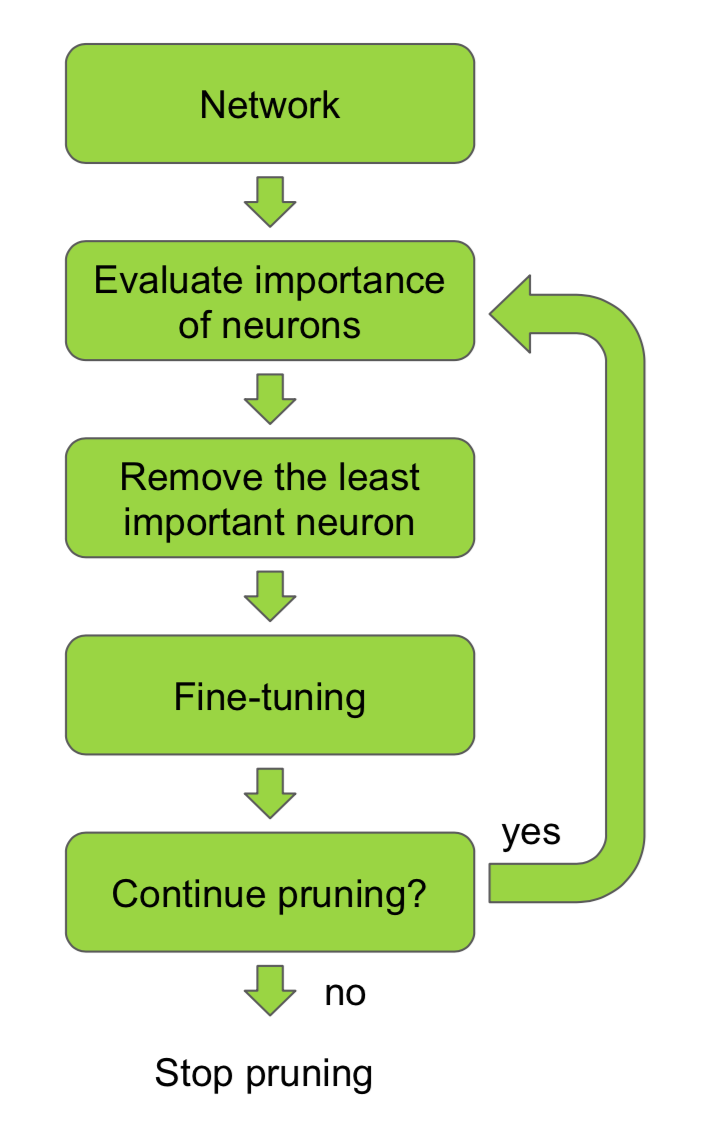
\includegraphics[width=4cm]{Figures/PruningMethod.png}
	\caption[Inference Optimisations]{Pruning method as a backward operator, presented in \cite{Molchanov2016}}
	\label{fig:PruningMethod}
\end{figure}

The last presented approach is \emph{quantisation} as it uses mixed-precision and uses it to optimise CNN models. This optimisation was closely studied since 2016 that was a year where many researchers studied the phenomenon. Starting in 2015 and 2016, Hubara, Courbariaux et al. \cite{Hubara2016, Courbariaux2015, Courbariaux2016} present the first works on \emph{QNNs}  and write the first training methodology for \emph{BNNs}.

Techniques have been presented the same year by Miyashita et al. \cite{Miyashita2016} to train \emph{QNNs}. In their work, they highlight a new logarithmic data representation to encode a neural network using 3-bits values. Their data representation consists of using \guille{non-uniform, base-2  logarithmic representation to encode weights, communicate activations and perform dot products}. They manage achieve higher classification accuracies than fixed-point at the same resolution and they propose a 5-bit representation that achieve higher test accuracy than 5-bit linear representation. Through their encoding, they manage to save space by encoding weights and activations in less space and save memory bandwidth by replacing the dot product (multiply accumulate) with a simpler operator for the logarithmic representation as shown on \emph{Figure} \ref{fig:DotProdLog}.

% LOG REPRESENTATION
\begin{figure}[htbp]
	\centering
		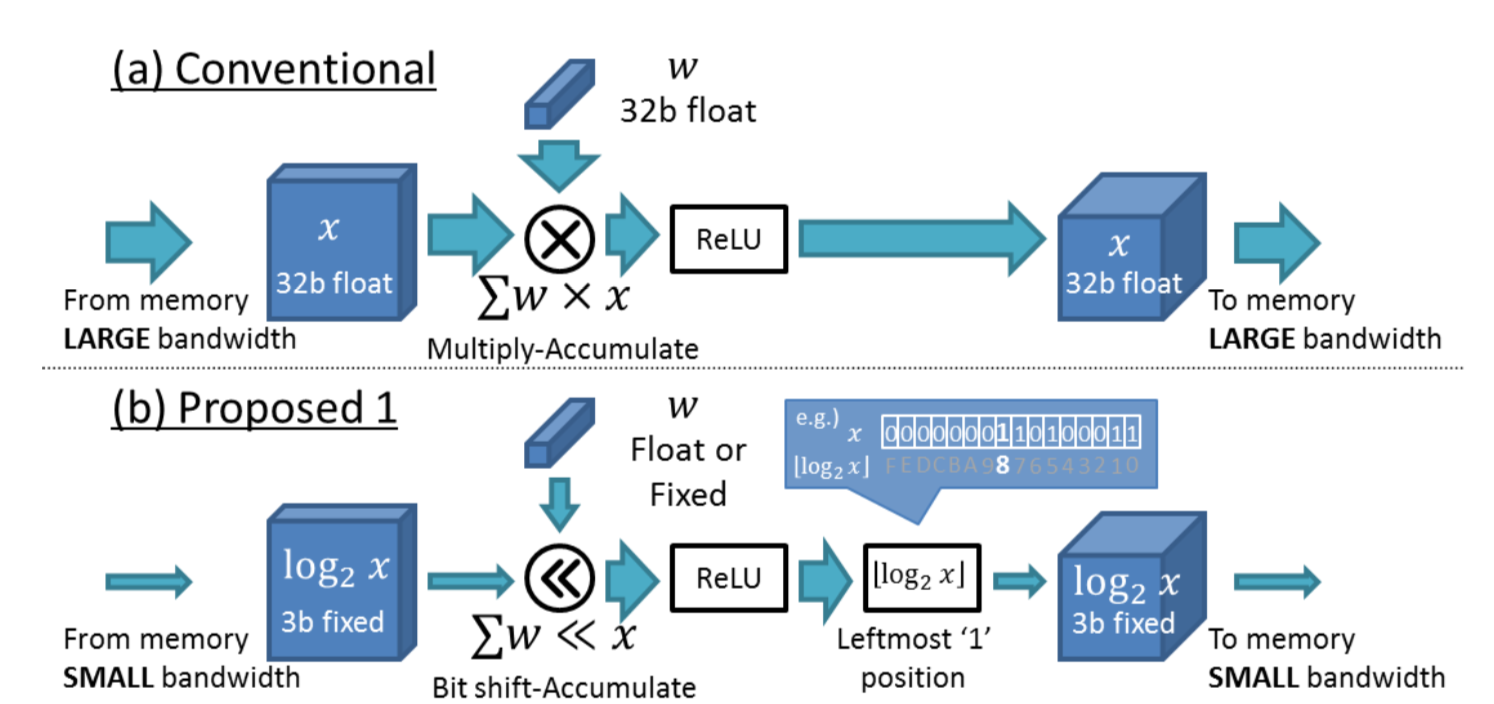
\includegraphics[width=12cm]{Figures/DotProdLog.png}
	\caption[Logarithmic Dot Product]{The Logarithmic way to perform Dot-Product \cite{Miyashita2016}}
	\label{fig:DotProdLog}
\end{figure}

Using yet another data representation, Micikevicius et al. \cite{Micikevicius2017} store weights, activations and gradients in IEEE half-precision nearly halving the memory requirements and speeding up the arithmetic. The authors propose three techniques to maintain the accuracy of the model. They maintain a single-precision copy of weights to accumulate the gradients, propose a loss-scaling to preserve low-magnitude gradients and use half-precision arithmetic that writes to single-precision arithmetic before writing the half-precision values to memory. A layer performs several operations in order to keep a high precision result, this behaviour is shown on \emph{Figure} \ref{fig:HPTraining}.

% LOG REPRESENTATION
\begin{figure}[htbp]
	\centering
		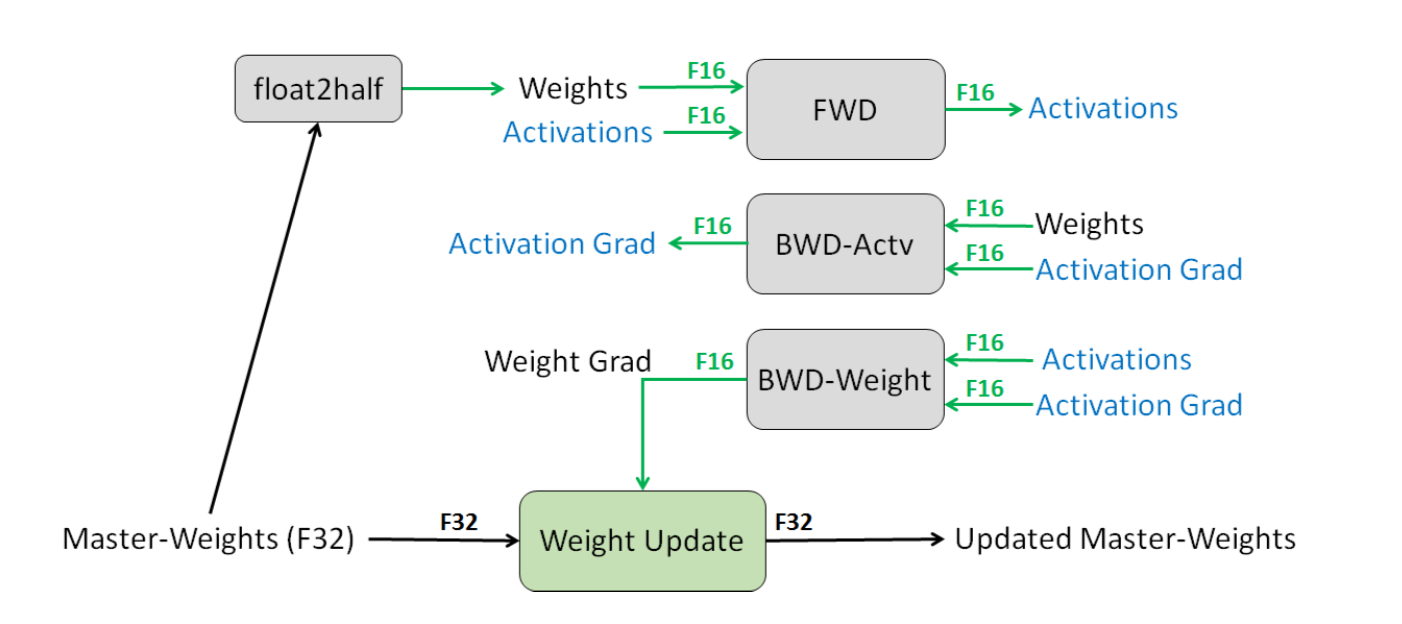
\includegraphics[width=10cm]{Figures/HPTraining.png}
	\caption[HPTraining]{Half-Precision Training  \cite{Micikevicius2017}}
	\label{fig:HPTraining}
\end{figure}

Rastegari et al. \cite{Rastegari2016} present \emph{Binary-Weights Networks}, on the same vein as Courabariaux et al. \cite{Courbariaux2016}. Their implementation however outperform the other of more than 16\% in top-1 accuracy. On the other hand, they present \emph{XNOR-Nets} that, for the first time, reduce dot-product operations to \emph{XNOR} operations followed by a \emph{Population Count (POPCount)} operator that counts the number of ones in the binarised vector. The \emph{XNOR-Nets} are using mostly bitwise operations to approximate convolutions and this enables a speed-up of approximately 58 times and enables \guille{the possibility of running state-of-the-art deep neural networks on CPU (rather than GPU) in real-time}.

Zhou et al. \cite{Zhou2016} present \emph{DoReFaNet}, a method to train neural network that have low bitwidth weights and low bitwidth activations. This is done by using low bitwidth gradients. During the backward pass, parameters gradients are quantised to low bitwidth numbers before being propagated to convolutional layers. They present a version of \emph{AlexNet} that has 1-bit weights, 2-bit activations that is trained from scratch using 6-bit gradients and manages to get 46.1\% top-1 accuracy on \emph{ImageNet}, a state-of-the-art performance.

Mixed-precision is extremely useful when dealing with \emph{inference} on low-space, low-energy hardware architectures. However, it can also be used to speed up the training times of deep neural networks on large datasets (such as \emph{ImageNet} for example). For now, training \emph{ResNet-50} on 8 Tesla P100 GPUs takes 29 hours \cite{He2016}. This time  impedes the research and development progress. Jia et al. \cite{Jia2018} present a novel mixed-precision training method along with an optimised all-reduce algorithm. Any neural network will have to use a version of an all-reduce algorithm, consisting of the sum of all the previous elements broadcasted to all the next elements. Using an optimised version of the algorithm will increase the performance of each layer separately and the whole system in the end. This method along with a \emph{Synchronised Stochastic Gradient Descent (SVG)} allows them to train the network extremely quickly on their setup (consisting of a cluster of 1024 Tesla P40 GPUs). Mixed-precision allowed them to speed-up the training to a point where they manage to train \emph{ResNet-50} in 15 minutes and \emph{AlexNet} in 4 minutes, both on the \emph{ImageNet} dataset.


%-----------------------------------
%	SECTION 3.3 - CNNs on FPGAs
%-----------------------------------

\section{CNNs on FPGAs}

Due to their heavy parallel affinity, CNNs can benefit from both GPUs \cite{Micikevicius2017, Jia2018, Kurth2018} and FPGAs \cite{Park2016, Liang2017, Colangelo2018, Jahanshahi2019, Bacchus2020} heavy parallelisation capabilities.
However, CNNs as stated in \cite{Jahanshahi2019}, \guille{CNN-based methods are computational-intensive and resource-consuming, and thus are hard to be integrated into embedded systems such as smartphones, smart glasses and robots}. FPGAs can counterbalance this issue by providing a tailored hardware representation of the CNN and making the most our of limited precision datatypes. They also appear as an in-between alternative over GPUs and under ASICs.

%--------------------------------------------
%	SUBSECTION 3.3.1 - Parallelisation Vectors
%--------------------------------------------

\subsection{Parallelisation Vectors}

Low-energy embedded systems can take advantage of the affinity of CNNs with parallelisation. This extensive concurrency can be used when parallelising from either \emph{Batch Parallelism} or \emph{Inter-Layer Parallelism}.

Batch size is an important parameter when looking at networks, it corresponds to \guille{a hyper-parameter that defines the number of samples to work through before updating the internal model parameters (weights)} \cite{MLMastery2019}. As stated in \cite{MLMastery2019}, the difference between a \emph{batch} and an \emph{epoch} is that an epoch consists of a full run through the training set while several batches can fit into an epoch. The batch size can divide the training in several types depending on the batch size:

\begin{itemize}
	\item \emph{Batch Gradient Descent}: Batch size = Size of the training set
	\item \emph{Stochastic Gradient Descent}: Batch size = 1
	\item \emph{Mini-batch Gradient Descent}: 1 $<$ Batch size $<$ Size of the training set
\end{itemize}

A CNN can simultaneously run the filters of the network on the instances of the same batch and obtain a significant acceleration when using batch processing. On the other hand, the structure of the network can be described as \guille{feed-forward}, meaning the output of layer $n$ is directly fed into layer $n+1$. A pipelined implementation can trigger the layer $n+1$ before the end of layer $n$ on selected instances.

The layers CONV are source of concurrency that can be exploited through the separation of the different planes the CONV layer uses (inter-FM), or the separation of the outputs of the layer (intra-FM). Moreover, the 3D-convolution can be expressed as a sum of 2D-convolutions that can be executed in parallel (inter-convolution) and the 2D-convolutions themselves can be pipelined concurrently (intra-convolution).

Many modern development frameworks implement a distributed version of optimisers and back-propagation to perform operations with \emph{MPI} or \emph{NCCL} for \emph{CUDA Tensors}. This allows both training and inference to be sped up by distributing their different heavy-load operations (multiply accumulate, dot-products, all-reduce, etc.). It also allows to separate the different instances from within the same batch to be run separately before gathering the resulting impact on the network parameters.

FPGAs run against several bottlenecks such as limited bandwidth and on-chip memory. However, due to their flexible nature, CNNs can be adapted to be run on them. Qiu et al. \cite{Qiu2016} show in their state-of-the-art study that the Convolutional layers are computationally-centric and Fully-Connected layers are memory-centric. This means that using any of the two layers will have to bring a concern on the associated bottleneck it holds as well.

%---------------------------------------------------------
%	SUBSECTION 3.3.2 - Training and Inference Optimisations
%---------------------------------------------------------

\subsection{Training and Inference Optimisations}

FPGAs provide an in-between solution between GPUs and ASICs. They can be used in both \emph{Training} and \emph{Inference} in order to process the different instances of the dataset they are being fed. This subsection will present the different training and inference optimisations that can be brought on FPGAs. As said earlier, the \emph{Inference} step is a critical spot of CNN implementations as it is required each time a new instance is presented to the system whereas the \emph{Training} step can be done once and for all. Increasing the performance of this step is crucial and can be done in several ways. First, the memory bandwidth is the bottleneck of several FPGA implementations. High number of memory reads or high number of weights stored result in a loss of performance. A caching strategy is often a nice answer to this kind of issues.

Next, the literature presents several optimisations strategies that will help the CNN perform best on an FPGA. Exporting a CNN to an FPGA consists in finding the most efficient way to map the CNN on the hardware architecture of the FPGA. The main strategies are listed beneath and presented in \emph{Figure} \ref{fig:InferenceOpt}. Several solutions found in the literature present combination of different strategies to perform best on a given architecture. Several methods have already been presented in the \emph{Optimisation Methods} subsection such as \emph{Pruning}, \emph{Compression} or \emph{Quantisation} with an FPGA note. \emph{Pruning} still has an FPGA implementation as presented by Fujii et al. \cite{Fujii2017} as well as an accelerator model proposed by Kang et al. \cite{Kang2019}. However, more FPGA-specific methods exist.

\begin{figure}[htbp]
	\centering
		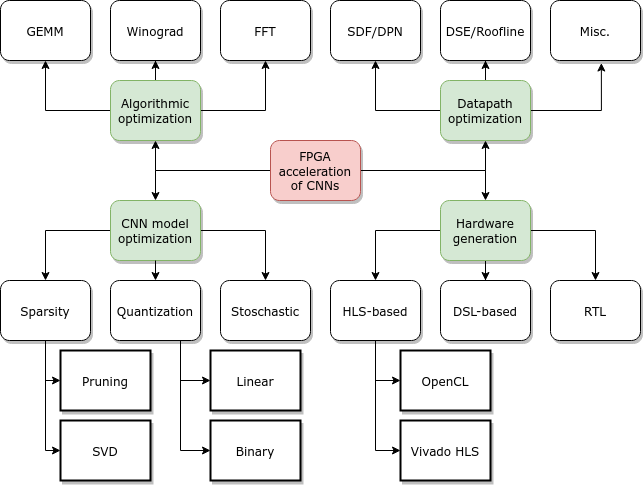
\includegraphics[width=.75\textwidth]{Figures/InferenceOpt1.png}
	\caption[Inference Optimisations]{Methods to accelerate an FPGA implementation \cite{Abdelouahab2018}}
	\label{fig:InferenceOpt}
\end{figure}

The main strategies specific to FPGAs are linked to \emph{Hardware Generation} and \emph{Data-path optimisations}. The first one, \emph{Hardware Generation}, depends on the way the configurable hardware will be used and tuned. As shown in \emph{Figure} \ref{fig:InferenceOpt}, several methods exist to reconfigure an FPGA. Some use \emph{High Level Synthesis} through either OpenCL or Vivado. These different frameworks and accelerators will be the focus of subsection \ref{fpga_framework}. On the other side, the \emph{Data-path optimisations} mainly revolve around the idea of loop optimisation. Several methods can be applied to the execution of nested loops to perform better on an FPGA. Loop optimisation comes in two different shapes: \emph{loop unrolling} and \emph{loop tiling}.

Unrolling a loop accelerates its execution at the cost of resource utilisation. Loop tiling consists of modifying the order of the different embedded loops in order to have the most expensive operations come all-together. These operations are \emph{DRAM (external memory)} accesses where the weights are stored since the FPGA cannot store them all with on-chip memory. An example of loop tiling can be seen on \emph{Figure} \ref{fig:LoopTiling}.

The settings of unroll and tiling factors will directly determine the number of \emph{Processing Elements (PE)} and their associated computing resources as well as the amount of DRAM accesses.

% Loop Tiling
\begin{figure}[htbp]
\centering
\begin{minipage}{.48\textwidth}
\begin{lstlisting}[style=CInputStyle]
// Ll: Layer
for (int l=0;l<L,l++){
// Lb : Batch
for (int b=0;b<B,l++){
// Ln: Y Depth
for (int n=0;n<N;n++){
// Lv: Y Columns
for (int v=0;v<V,v++){
// Lu: Y Raws
for (int u=0;u<U,u++){
// Lc: X Depth
for (int c=0;n<C;c++){
// Lj: Theta Columns
for (int j=0;j<J,j++){
// Lk: Theta Raws
for (int k=0;k<K,k++){
  Y[b,l,n,v,u] += X[b,l,c,v+j,u+k] *
        Theta[l,n,c,j,k]
}}}}}}}
\end{lstlisting}
\end{minipage}
\hfill
\begin{minipage}{.48\textwidth}
\begin{lstlisting}[style=CInputStyle]
for (int n=0;n<N;n+=Tn){
for (int v=0;v<V,v+=Tv){
for (int u=0;u<U,u+=Tu){
for (int c=0;n<C;c+=Tc){
  // DRAM: Load in on-chip buffer the tiles
  // X[l,c:c+Tc,v:v+Tv,u:u+Tu]
  // Theta [l,n:n+Tn,c:c+Tc,j,k]
  // Process on-chip tiles
  for (int tn=0;tn<Tn;tn++){
  for (int tv=0;tv<Tv,tv++){
  for (int tu=0;tu<Tu,tu++){
  for (int tc=0;tn<Tc;tc++){
  for (int j=0;j<J,j++){
  for (int k=0;k<K,k++){
    Y[l,tn,tv,tu] += X[l,tc,tv+j,tu+k] *
            Theta[l,tn,tc,j,k];
  }}}}}}
  // DRAM: Store output tile
}}}}
\end{lstlisting}
\end{minipage}
\caption[LoopTiling]{Loop Tiling Example \cite{Abdelouahab2018}}
	\label{fig:LoopTiling}
\end{figure}

Now if we look more closely on \emph{Quantisation} methods applied to FPGAs, the literature present several works:

Colangelo et al. \cite{Colangelo2018} present a CNN mapping to a reconfigurable architecture in order to use sub 8-bit activation and weights. In order to use binary- or ternary-weighted neural networks, they cap their sizes to respectively 1 and 2-bits. Using this type of limited numeric precision can only be fully optimised with FPGAs and the authors show that they manage to get an optimisation of \guille{the bandwidth, memory, power and computation savings}.
uning 
Zhao et al. \cite{Zhao2016} propose \emph{F-CNN}, a framework to train CNNs on FPGAs. Their design makes available highly customisable modules that will be optimised to maximise performance under the constraints of bandwidth and hardware resources. The authors state that the introduction of mixed-precision will be the next step of optimisation of their design. Moreover, the use of they prove their design is more performant than CPUs and less expensive in terms of energy than GPUs. \emph{F-CNN} reconfigures a streaming datapath at runtime to cover the training tasks for the various layers in a CNN.

Jahanshahi et al. \cite{Jahanshahi2019} propose a CNN accelerator tool. It generates the hardware description for a CNN to be programmed on a target FPGA. The software uses an API the developer can use to enter the available resources. The software will then generate the hardware description and run a simulation to adjust the precision and minimise the classification error. The whole system is shown to be more performant on a half-precision fixed-point representation rather than using single-precision floating-point data: 3\% accuracy loss in exchange for 15.75x speedup.

The even more agressive vision of quantisation with binary parameters as set by Courbariaux et al. \cite{Courbariaux2016} was conducted on GPUs but their FPGA counterpart have been developed later on. Liang et al. \cite{Liang2017} present a BNN implemented on an FPGA and the benchmarked results show an improvement in speed and energy efficiency over other computing platforms.


%--------------------------------------------------------
%	SUBSECTION 3.3.3 - FPGA Frameworks
%--------------------------------------------------------

\subsection{FPGA Frameworks}\label{fpga_framework}

In 2016, the same year \emph{QNNs} began to gain attraction and credibility, FPGA frameworks emerged to take advantage of FPGA capabilities along with mixed-precision. The first works in the fiels are \emph{YodaNN} \cite{Andri2016} and \emph{F-CNN} \cite{Zhao2016}. Andri et al. set up \emph{YodaNN}, an accelerator optimised for \emph{BNNs} and one of the first implementations. Zhao et al. \cite{Zhao2016} designed F-CNN, the first FPGA framework to train CNNS. Later on, Wang et al. \cite{Wang2018} developed a design flow for extremely low-bit neural networks that focuses on quantisation in both training and FPGA deployment. They aimed at strict resources and power constraints in order to provide a design to the developer.

The next year, two initiatives are launched in order to perform an automatic mapping of a CNN down to its hardware counterpart on an actual hardware architecture. \emph{fpgaConvNet} is created by Venieris et al. \cite{Venieris2017}. It automates the mapping of CNNs on FPGAs using application-level needs (throughput, latency or multiobjective criteria). It uses a paradigm called \emph{Synchronous Dataflow (SDF)} and defines a set of \emph{SDF} transformations in order to efficiently explore the design space. \emph{fpgaConvNet} implements four different transformations the network will be run through: \guille{\emph{graph partitioning}with reconfiguration, coarse-grain \emph{folding}, fine-grained \emph{folding} and weights \emph{reloading}}. Those four different transformations can be seen on \emph{Figure} \ref{fig:fpgaConvNetTransformations} respectively (a), (b), (b) and (c).

\begin{figure}[htbp]
	\centering
		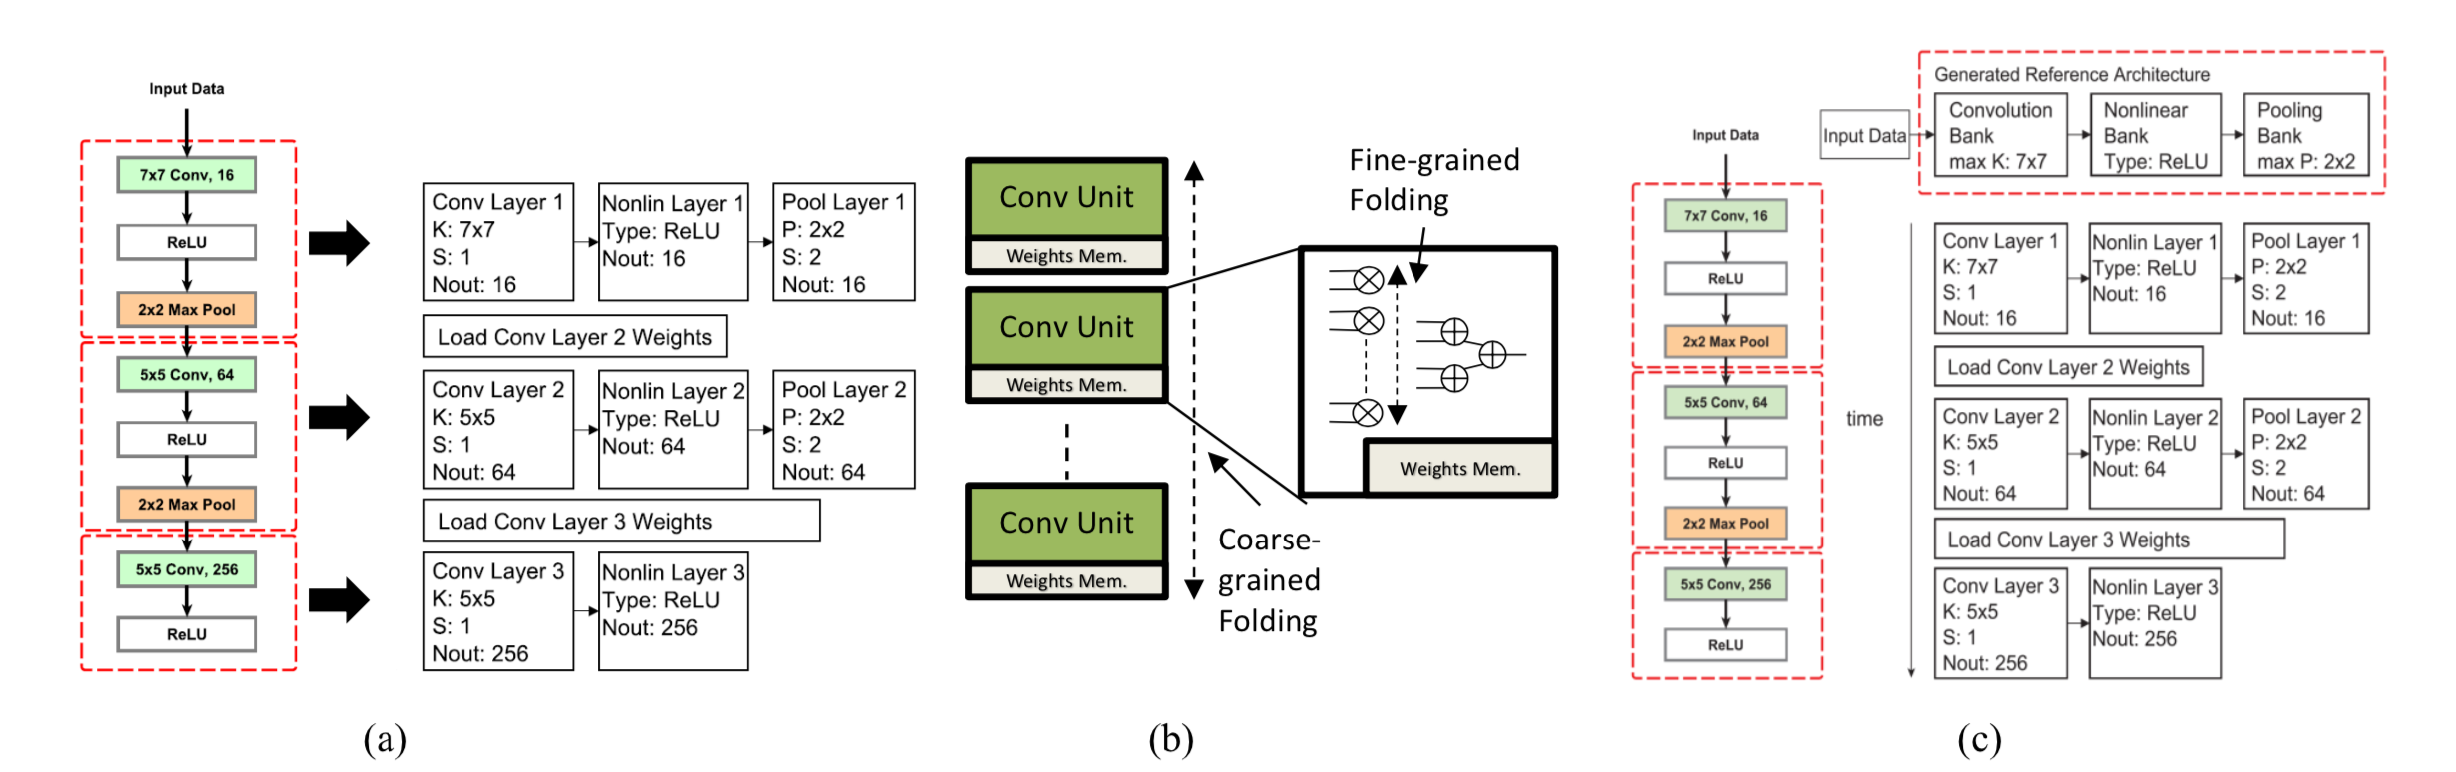
\includegraphics[width=\textwidth]{Figures/fpgaConvNetTransformations.png}
	\caption[Inference Optimisations]{Different transformations used by \emph{fpgaConvNet} \cite{Venieris2017}}
	\label{fig:fpgaConvNetTransformations}
\end{figure}


The tool will separate the CNN into different subgraphs that will be tailored specifically to the target architecture. The execution of each subgraph requires a reconfiguration of the FPGA and \emph{fpgaConvNet} performs a batch-processing of the subgraph in order to amortise reconfiguration times. This transformation is called \emph{graph partitioning}. Next, \emph{coarse-grain folding} enables the tuning of the number of coarse units for each layer. It spans a fully parallel implementation down to a single, time-shared unit. Then, \emph{fine-grained folding} allows the configuration of the dot-product implementation in the convolutional units of a layer. It spans a fully parallel implementation down to a single , time-shared multiply-accumulate unit. Finally, the \emph{weights reloading} is similar to the first transformation in the sense that it will separate the network in several parts but will this time single flexible reference to all the weights of the network. This allows a layer to use the weights of the last layer without reloading them in memory.

In the other hand, \emph{FINN} \cite{Umuroglu2017a} has been developed as an open-source framework by the FPGA manufacturer Xilinx. It works as a network compression tool especially tailored for FPGAs and have been actively under development with extensions to quantised networks \cite{Blott2018} or Long Short-Term Memory (LSTM) networks \cite{Rybalkin2018}. It has been developed in order to propose a complete workflow to its users. First, another tool developed by Xilinx can be used in order to train quantised networks, \emph{Brevitas}. This tool produces a network in an intermediate representation with annotation for the FPGA framework. \emph{FINN} loads this intermediate representation and, in the same way \emph{fpgaConvNet} would do, runs the network through a series of different transformations. \emph{Figure} \ref{fig:FinnWorkflow} presents the whole workflow.

\begin{figure}[htbp]
	\centering
		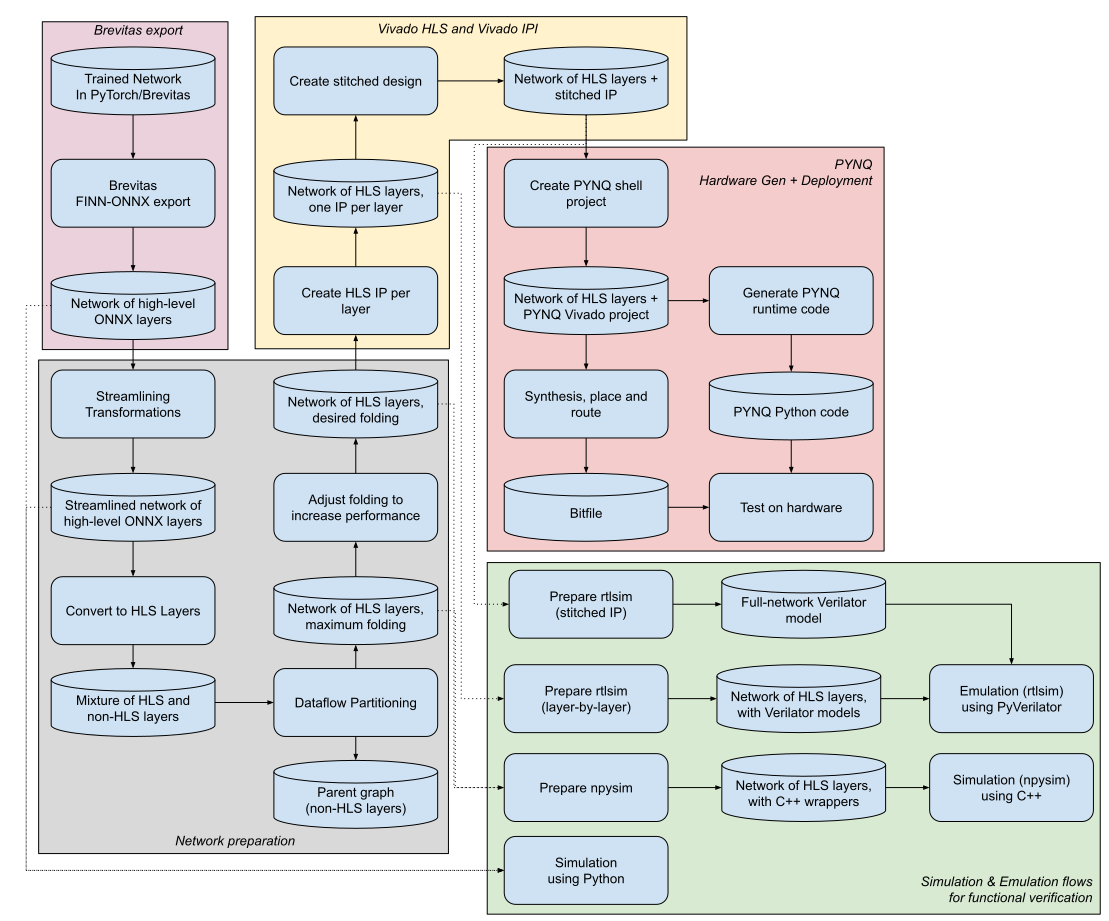
\includegraphics[width=\textwidth]{Figures/FinnWorkflow.png}
	\caption[Inference Optimisations]{FINN workflow as presented in \cite{Umuroglu2017a, Blott2018}}
	\label{fig:FinnWorkflow}
\end{figure}

The first transformations are called \emph{tidy-up} and consists of renaming the different nodes in the intermediate representation, renaming the tensors and infering shapes and data types. Next, another series of transformations arrives under the name of \emph{streamlining}, or a way to eliminate floating-point operations. It moves the operations around and collapses them into \emph{multithresholding} nodes. Next, the layers are converted into \emph{High-Level Synthesis (HLS)} layers, seprating the overall graph into a mixture of \emph{HLS} nodes and \emph{non-HLS} nodes. Then, the graph is split in two parts, one containing \emph{HLS} nodes that will be executed on the board while others are kept as they are. This step is called \emph{dataflow partitioning}. Finally, a \emph{folding} step is provided, where parameters such as the number of \emph{PEs (Processing Elements)} or \emph{SIMDs (Single Instruction Multiple Data)} can be tuned. The network will then be processed layer by layer and converted to a hardware counterpart. This counterpart consists of a stitched \emph{IP (Intellectual Property)} composed by other \emph{IPs}, one per layer. \emph{IPs} are custom blocks that can be processed by an FPGA.

An interesting difference between the two frameworks is the \emph{FINN} ability to simulate the steps during the workflow. This verification (as shown in the green bottom-left part of \emph{Figure} \ref{fig:FinnWorkflow}) can be performed in three different ways: a simulation using Python after the network is exported in intermediate representation, a simulation in C++ when the network contains the \emph{HLS} nodes and an emulation using \emph{PyVerilator} when the different IP blocks (one per layer) are generated. \emph{FINN} also comes with a dedicated trainer for networks. This trainer provides \guille{drop-in} replacements for PyTorch layers.

In 2019, Ding et al. \cite{Ding2019} propose a \guille{Resource-aware, efficient quantisation framework} for object detection on FPGAs. They present an extension and automation of the YOLO model used in the object detection field. Jahanshahi et al. \cite{Jahanshahi2019} present TinyCNN, a modular CNN framework using 16-bit fixed-point data. Zhao et al. \cite{Zhao2019} present Tomato, \guille{a framework designed to automate the process of generating efficient CNN accelerators}. Tomato uses different arithmetics and precisions within each Convolutional layer. This is the first multi-precision multi-arithmetic auto-generation framework for CNNs.

Between all these different frameworks, \emph{FINN} seems to be the one that encounter a growing community. This may be due to the fact that the initiative is pushed by Xilinx, a well-known FPGA manufacturer. Their tools provide interconnection, whether it is between their boards and FINN or the integration with their GUI \emph{Vivado} and \emph{Vitis}.

%------------------------------------------------------
%	SUBSECTION 3.4 - Takeaway from the Literature Review
%------------------------------------------------------

\section{Takeaway from the Literature Review}
In this \emph{Background} and \emph{Literature Review}, the focus went from the background of number representation, machine learning and hardware architectures to the underlying link between them, mixed-precision. The next part showed the different ways to both use mixed-precision in serious scientific computations and apply it to practical machine learning. The final parts present the works made to optimise both training and inference for neural network on different architectures. The final point was to present the existing tools to port a mixed-precision network to a \guille{by-default} mixed-precision architecture, FPGAs.

Benchmarking and optimisation are extremely important topics in the field of machine learning when it comes to evaluation of a new set up, architecture or optimisation methods. Extensive benchmarking has been done on well-known network architectures or datasets and this provides an easy insight on what went better and what went worse. However, very few effort has been put together to compare development frameworks implementation between them. This translates in a lack of answers from industrials or companies to choose concretely for a solution before running into an artificial intelligence or machine learning project. For now, the question is \guille{Which company from the GAFA would you like to support by using their framework?} rather than actual performance. The difference also comes from the tools developed on top of these frameworks.

When looking at optimisation methods, parameters are empirically chosen and few benchmarks exist to test them and their reliability. Several articles from the literature often propose an empirical choice in parameters size along with the architecture and performance they got out of the experiment. Bacchus et al. \cite{Bacchus2020} benchmark the trade-offs between training-time, hardware efficiency and accuracy in QNNs while varying the size of the parameters. The work proposed could be extended with new frameworks, architectures and  datasets. The experiment could be reconducted on different architectures and datasets in order to confirm or invalidate the sweet spots found. An extension to \emph{fpgaConvNet} or \emph{Brevitas} (with PyTorch) could widen the benchmark. In fact, if binarisation is known to be effective when coming from a 32-bit floating point representation. However, little data covers the impact of the quantisation of weights, as opposed to the impact of the quantisation of activations and what would a sweet spot be. Many factors come into play: network architecture, dataset, optimiser, loss function, quantisation, transformations pre- and post-training as well as hardware deployment methods.

There is room for benchmarking state-of-the-art implementations of \emph{QNNs} on FPGAs and their associated frameworks. FINN seems to be the one that chose to be developed in an open-source way, with an extension to a well-known framework (PyTorch) and the use of a common intermediate representation. Creating a scalable benchmark that could be given a network architecture, dataset, quantisations of weights and activations as well as training time would allow proper testing of a framework and show the flexibility of such a framework.

\chapter{Requirements Analysis} % Main chapter title

\label{Chapter4} % For referencing this chapter elsewhere, use \ref{Chapter3}

\lhead{Chapter 4. \emph{Requirements Analysis}}


This chapter looks over the aims and objectives set in the \emph{Introduction} and translates them into requirements and use cases in the first part. The second part is centred around the methodology the project will be evaluated with. The third and final part will enumerate the needed deliverables.
%----------------------------------------------------------------------------------------
%	SECTION 4.1 - Project Goals
%----------------------------------------------------------------------------------------

\section{Project Goals}

The aims and objectives defined at first are then translated into requirements using \emph{functional analysis}, a method borrowed to the field of software engineering. All the functional and non-functional requirements are then discussed along with the requirements table.

%----------------------------------------------------------------------------------------
%	SUBSECTION 4.1.1 - Aims and Objectives
%----------------------------------------------------------------------------------------

\subsection{Aims and Objectives}

Taking from the \textbf{Aims} defined in Chapter \ref{Chapter1}, we derive the objectives and define the requirements for the project.

\textbf{Objectives}

\begin{enumerate}
  \item Implement a CNN on an FPGA
  \begin{enumerate}
    \item Hardware architectures: PYNQ-Z1, Zedboard Zynq 7000 and Digilent Nexys A7
    \item Development Framework: \emph{Brevitas} over PyTorch
    \item Acceleration Framework: \emph{FINN}
    \item Datasets: MNIST (or similar), CIFAR-10 and GTSRB
    \item Network Architectures: Succession of FC layers, Simple ConvNet (similar to LeNet), MobilenetV1
  \end{enumerate}
  \item Determine the impact of the size of parameters linked to the application.
  \begin{enumerate}
    \item Weights
    \item Activation Function
    \item Training Time
  \end{enumerate}
  \item Measure the metrics of the associated application as compared to the literature.
  \begin{enumerate}
    \item Throughput
    \item Accuracy
    \item Energy
    \item Hardware Utilisation
    \item Compression Ratio
  \end{enumerate}
  \item Confront the results to the state-of-the-art comparable experimental results.
\end{enumerate}

The above objectives consist of an extension of the \cite{Bacchus2020} article in order to benchmark a similar setup with an extended framework, PyTorch extension \emph{Brevitas}. These objectives roughly translate into the design and development of a benchmark tool that should be able to use \emph{Brevitas} in order to design and train \emph{QNNs}. Next, the benchmark tool should be able to export the desired network to the \emph{Intermediate Representation}. Finally the sequence of transformations and proper folding has to be set up through \emph{FINN} in order to complete the workflow and port the network to the FPGA board.

%----------------------------------------------------------------------------------------
%	SUBSECTION 4.1.2 - Requirements
%----------------------------------------------------------------------------------------

\subsection{Requirements}

The above objectives translate into requirements for the actual final software.

\textbf{Requirements Table} The \emph{Table} \ref{tab:RequirementsTable} specifies the requirements that the developed system should fulfill. It does not give an indication of how the requirements will be met but instead explains the reasons of its existence. Each requirement has an identifier, a name, a priority rank (0 being the highest) and an explanation.

% REWORK PRIORITIES
\begin{table}[!]
  \centering
  \resizebox{\textwidth}{!}{
  \begin{tabular}{| c c l c c |}
    \hline
    \textbf{ID}                   & \textbf{Name}                           & \textbf{Description}                                                   & \textbf{Type}               & \textbf{Justification} \\ \hline
    \multirow{2}{*}{\textbf{R0}}  & \multirow{2}{*}{\emph{LitNetwork}}      & The system should use                                                  & \multirow{2}{*}{Constraint} & \multirow{2}{*}{Literature review} \\
                                  &                                         & network architectures comparable to the literature                     &                             & \\ \hline
    \multirow{2}{*}{\textbf{R1}}  & \multirow{2}{*}{\emph{LitDataset}}      & The system should use                                                  & \multirow{2}{*}{Constraint} & \multirow{2}{*}{Literature review} \\
                                  &                                         & datasets comparable to the literature                                  &                             & \\ \hline
    \multirow{2}{*}{\textbf{R2}}  & \multirow{2}{*}{\emph{LitDevFramework}} & The system should use                                                  & \multirow{2}{*}{Constraint} & \multirow{2}{*}{Literature review} \\
                                  &                                         & a development framework presented the literature                       &                             & \\ \hline
    \multirow{2}{*}{\textbf{R3}}  & \multirow{2}{*}{\emph{LitAccFramework}} & The system should use                                                  & \multirow{2}{*}{Constraint} & \multirow{2}{*}{Literature review} \\
                                  &                                         & an acceleration framework presented the literature                     &                             & \\ \hline
    \multirow{2}{*}{\textbf{R4}}  & \multirow{2}{*}{\emph{LitArch}}         & The system should use a known hardware architecture                    & \multirow{2}{*}{Constraint} & \multirow{2}{*}{Literature review} \\
                                  &                                         & or at least equivalent to the literature &                             & \\ \hline
    \multirow{2}{*}{\textbf{R5}}  & \multirow{2}{*}{\emph{TestParam}}       & The system should evaluate                                             & \multirow{2}{*}{Constraint} & \multirow{2}{*}{User requirement} \\
                                  &                                         & the impact of the tuning parameters                                    &                             & \\ \hline
    \multirow{2}{*}{\textbf{R6}}  & \multirow{2}{*}{\emph{TestOptMeth}}     & The system should evaluate                                             & \multirow{2}{*}{Constraint} & \multirow{2}{*}{User requirement} \\
                                  &                                         & the impact of the optimisation methods                                 &                             & \\ \hline
    \multirow{2}{*}{\textbf{R7}}  & \multirow{2}{*}{\emph{TestHardDes}}     & The system should evaluate                                             & \multirow{2}{*}{Constraint} & \multirow{2}{*}{User requirement} \\
                                  &                                         & the impact of the hardware design                                      &                             & \\ \hline
    \multirow{2}{*}{\textbf{R8}}  & \multirow{2}{*}{\emph{ExpTrain}}        & The system should lead the experiment through a sound,                 & \multirow{2}{*}{Constraint} & Meaningful \\
                                  &                                         & consistent and replicable training process                             &                             & experimental process\\\hline
    \multirow{2}{*}{\textbf{R9}}  & \multirow{2}{*}{\emph{ExpDeploy}}       & The system should lead the experiment through a sound,                 & \multirow{2}{*}{Constraint} & Meaningful \\
                                  &                                         & consistent and replicable deployment process                           &                             & experimental process\\ \hline
    \multirow{2}{*}{\textbf{R10}} & \multirow{2}{*}{\emph{ResGuide}}        & The system should help                                                 & \multirow{2}{*}{Constraint} & \multirow{2}{*}{Exploitable results}\\
                                  &                                         & create guidelines with the results                                     &                             & \\ \hline
    \multirow{2}{*}{\textbf{R11}} & \multirow{2}{*}{\emph{ResComp}}         & The system should create                                               & \multirow{2}{*}{Constraint} & \multirow{2}{*}{Exploitable results}\\
                                  &                                         & results comparable to the literature                                   &                             & \\ \hline
  \end{tabular}
  }
\caption[Requirements Table]{Requirements Table}
  \label{tab:RequirementsTable}
\end{table}

The projected counterparts to the first requirements are the following:
\begin{itemize}
  \item \textbf{R0}: \emph{TFC}, \emph{CNV}, \emph{LeNet5}, \emph{VGG} and/or \emph{MobilenetV1}
  \item \textbf{R1}: \emph{MNIST (or similar)}, \emph{CIFAR-10}, \emph{GTSRB} and/or \emph{SVHN}
  \item \textbf{R2}: \emph{PyTorch} extension \emph{Brevitas}
  \item \textbf{R3}: Xilinx acceleration framework \emph{FINN}
  \item \textbf{R4}: \emph{PYNQ-Z1}, \emph{Zedboard Zynq-7000} and/or \emph{Diligent Nexys-A7}
\end{itemize}

The projected deliverables for the \emph{Dissertation Thesis} are this given report as well as the \emph{Ethics Forms}. Additionally, the developed \emph{Software} and obtained results are provided. The results go along with discussion, evaluation and a presentation of the future works that can extend the project.

%----------------------------------------------------------------------------------------
%	SECTION 4.2 - Evaluation Methodology
%----------------------------------------------------------------------------------------

\section{Evaluation Methodology}

This section will provide methods, criteria and metrics to evaluate the end product and the deliverables.

%----------------------------------------------------------------------------------------
%	SUBSECTION 4.2.1 - Comparison
%----------------------------------------------------------------------------------------

\subsection{Comparison}

The results of the study and the values obtained will be compared to state-of-the-art studies and methods. The main works used for the comparison will be similar CNNs applied on different parallel architectures, from GPUs \cite{Micikevicius2017, Jia2018, Kurth2018} to FPGAs \cite{Zhao2016, Colangelo2018, Jahanshahi2019, Bacchus2020}. The different works will be compared on the basis of:
\begin{itemize}
  \item \textbf{Quantisation} of the parameters
  \item \textbf{Accuracy} of the network on the provided dataset
  \item \textbf{Throughput} of the instances through the deployed network
  \item \textbf{Energy} consumed by the inference
  \item \textbf{Hardware Utilisation} of the network on the hardware architecture
\end{itemize}

%----------------------------------------------------------------------------------------
%	SUBSECTION 4.2.2 - Requirements
%----------------------------------------------------------------------------------------

\subsection{Requirements}

Each requirement from the table will be examined later on and run against the actual product. A decision will be made on wether the requirement has been met, partially fulfilled or unsatisfied. A justification will have to be given for the unsatisfied requirements. Modifications to the actual requirements will have to be justified along with why the previous one was not fitting the final product.

%----------------------------------------------------------------------------------------
%	SUBSECTION 4.2.3 - Quality
%----------------------------------------------------------------------------------------

\subsection{Quality}

The scientific process will be reviewed to check if it complies to good practices and sound methodology. The results have to be reproducible and performed under a sound experimental process. Any parameter or configuration that might have been overlooked will have to be stated as so and justified. This reproducibility comes through a well-defined training process and an equally well-defined deployment process.

% Chapter Template

\chapter{Professional, Legal, Ethical and Social issues} % Main chapthe scaler title

\label{Chapter5} % For referencing this chapter elsewhere, use \ref{Chapter4}

\lhead{Chapter 5. \emph{PLES}}

%----------------------------------------------------------------------------------------
%	SECTION 5.1 - Professional Issues
%----------------------------------------------------------------------------------------

\section{Professional Issues}

The experimental process to obtain the results will establish specific hardware and software configurations. The specific configurations will be run against each other in order to establish guidelines. Those guidelines will take in account the evaluated parameters and draw conclusions on them and their impact on the overall system and performance.

Each piece of the tool and its implications will be tested and evaluated against other results from the literature. The configurations, if stated specifically, will help future research avoid duplication. Potential researchers can consider parameters that were overlooked in this study. Every experiment will be ensured to be reproducible and scientifically sound. Credible work has to be proposed in order to be taken in account by the literature

%----------------------------------------------------------------------------------------
%	SECTION 5.2 - Legal Issues
%----------------------------------------------------------------------------------------

\section{Legal Issues}

The project will be fully developed under a GNU GPLv3 license \cite{GNUGPL}. The objective of this license is to allow complete use of the source code and modifications. It allows:

\begin{itemize}
  \item \textbf{Commercial use}: The software can be used for commercial purposes.
  \item \textbf{Distribution:} The software may be distributed.
  \item \textbf{Modification:} The software may be modified.
  \item \textbf{Patent use:} The license provides an express grant of patent rights from the contributors.
  \item \textbf{Private use:} The software may be used and modified in private.
\end{itemize}

Under the following conditions:

\begin{itemize}
  \item \textbf{Disclose source:} Source code must be made available when the software is distributed.
  \item \textbf{License and copyright notice:} A copy of the license and copyright must be included with the software.
  \item \textbf{Same license:} Modifications must be released under the same license when distributing the software.
  \item \textbf{State changes:} Changes to the code must be documented.
\end{itemize}

The limitations of this license for the original developer can be met when looking at liability or warranty. This license includes a limitation of liability and explicitly states that no warranties are provided.


%----------------------------------------------------------------------------------------
%	SECTION 5.3 - Ethical Issues
%----------------------------------------------------------------------------------------

\section{Ethical Issues}

Providing guidelines on how reduced precision can impact performance will also highlight which parameters have an overall higher impact on the final performance. Since the goal of the study is to find the smallest size of each of the parameter without reducing the final precision too much and increasing the overall performance. Ranking parameters will give potential attackers hints on the importance of parameters. An alteration in the precision of a specific parameter can have a much higher impact when following the provided guidelines.

Moreover, since FPGAs are reconfigurable pieces of hardware, each one of the design will be tailored to the specific needs of the application. This means no superfluous space will be allocated and that overflow will have a considerable impact on the system. The use of reduced precision will have to block any attempt to downgrade precision or access restricted spaces of the hardware.

Since FPGAs are slowly developing their commercial use, fewer security measures are actually put in action. The project will have to state how precautions can be taken and how to protect the system against some attacks on precision or system integrity.

%----------------------------------------------------------------------------------------
%	SECTION 5.4 - Social Issues
%----------------------------------------------------------------------------------------

\section{Social Issues}

Machine learning and especially deep learning can be applied to nearly all computationally-demanding actions. Including speech processing, image recognition or object detection for example. These applications are more and more demanded and demanding in terms of performance and portability. Any improvement to the network setup and training process will have a heavy impact on any deep learning application.

Tailoring Neural Networks on hardware of restricted size helps portability and will be proven to increase performance. This means that the implications of the project will have a heavy impact on how to design an implication. Related works providing network frameworks on FPGAs \cite{Zhao2016, Colangelo2018, Jahanshahi2019} make the most performant designs accessible to as many people as possible for their application. However, as it is the case with every novel implementation, security guidelines have to be established. Potential flaws have to be detected and included in guidelines, early in the development process. FPGAs will gain increasing attention in the following years and this means stricter protections should be presented.

\chapter{Implementation} % Main chapter title

\label{Chapter6} % For referencing this chapter elsewhere, use \ref{Chapters}

\lhead{Chapter 6. \emph{Implementation}}

%----------------------------------------------------------------------------------------
%	SECTION 6.1
%----------------------------------------------------------------------------------------

\section{Frame}

This section comes after the literature review and requirements analysis to present the frame the software implementation will be developed on. This section will first go through the motivations in the choice of the frame as well as some perspective to move away from the objective and cover what will not be issued.

%-----------------------------------
%	SUBSECTION 6.1.1 - Motivations
%-----------------------------------

\subsection{Motivations}

Two objectives were set by missing information from the literature review. First, whether it is for development or acceleration frameworks, few benchmarks compare a similar implementation implemented in different frameworks. In terms of acceleration frameworks, this is due to the fact that few of them have opened their source code, making it time-consuming for one to perform a correct benchmark of the different frameworks. The other objective is to assess the importance of quantisation. While it has been proven that \emph{QNNs} could achieve the same accuracy and better throughput than classic \emph{CNNs}, few effort has been put in assessing the benefits and finding the best tailored precision for one's application.

Very few benchmarks exist on existing technologies, whether it is on development frameworks, or acceleration frameworks. The presentation of an accelerator often differs a lot from associated works and only state-of-the-art networks accuracy and throughputs are compared on simple architectures. Few projects seem to grow from the article they emerged from. \emph{YodaNN} \cite{Andri2016} does not provide any code outside of the article, neither does \emph{F-CNN} \cite{Zhao2016}. \emph{Tomato} \cite{Zhao2019}, \emph{TinyCNN} \cite{Jahanshahi2019} and \emph{fpgaConvNet} \cite{Venieris2017} face the same issue and make any comparison between the different frameworks very time-consuming. Only \emph{FINN} \cite{Umuroglu2017a, Blott2018} is still in active development and open-source.

Setting a benchmark from the open-source acceleration framework can help any external user have both a direct implementation of the framework as well as backed-up arguments on why it can help deploy one's application, at what cost and compared to state-of-the-art implementation. While the first objective presented earlier would be too time-consuming to complete, the second one is made possible through the usage of the open-source accelerator.

The main motivations taken in consideration when setting up the \emph{Brevitas} / \emph{FINN} benchmark is to provide an insight on the Xilinx tools and their workflow. This is important because widening the audience of the tool by presenting its capabilities allows both companies to be interested in the product as well as individuals to contribute to the project since it is open-source. The \emph{FINN} project started in September 2018 and has been in development ever since. The first version has been deprecated and a new direction is taken in 2019. The project is now using \emph{Brevitas} \cite{Pappalardo2020}, a PyTorch extension to perform the training and quantisation. \emph{FINN} is aiming at providing a clear acceleration of inference by deploying a network on an FPGA board. Both projects are open-source and can be found in their respective repositories on GitHub: \emph{FINN} \cite{FINNRepo} and \emph{Brevitas} \cite{BrevitasRepo}.

%--------------------------------------
%	SUBSECTION 6.1.2 - About Perspective
%--------------------------------------

\subsection{About Perspective}

Several papers present methods to \emph{train} networks on FPGAs \cite{Colangelo2018, Zhao2016, Jahanshahi2019}. However, while \emph{Brevitas} allows the training of \emph{QNNs}, it does not map the network on FPGAs at training time. It is expected to train the network on another hardware architecture (CPU(s) or GPU(s)) as PyTorch would expect and can handle. On the other hand, both \emph{Brevitas} and \emph{FINN} are in active development and in early phases of their development cycle. Version 0.3 of both tools has been released in late May this year.

%----------------------------------------------------------------------------------------
%	SECTION 6.2 - Workflow
%----------------------------------------------------------------------------------------

\section{Workflow}

This section will present the whole workflow \emph{Brevitas} / \emph{FINN} put into place. By first going through the \emph{QNN} designer and trainer that is \emph{Brevitas}, the quantised neural network is translated into the intermediate representation, \emph{ONNX}. The resulting intermediate representation can then be imported by \emph{FINN}. \emph{FINN} will perform several transformations and deploy part of the resulting graph on the associated FPGA.

%-----------------------------------
%	SUBSECTION 6.2.1 - Brevitas
%-----------------------------------

\subsection{Brevitas}

\emph{Brevitas} has been developed with the idea of corresponding to a \guille{drop-in} replacement of PyTorch. This means that it ensures that PyTorch functionalities will be kept, even when working with reduced-precision layers. \emph{Brevitas} implements a set of building blocks to model a reduced precision hardware data-path at training time. While partially biased towards modelling data-flow-style, very low-precision implementations, the building blocks can be parametrised and assembled together to target all sorts of reduced precision hardware.

The implementation sets up several design principles: idiomatic PyTorch if possible, modularity first at the cost of some verbosity and a focus on easy extendability. \emph{Brevitas} features many different ideas such as extracted from its presentation:
\begin{itemize}
  \item \textbf{Quantisation Type}: Binary, ternary or uniform integer.
  \item \textbf{Target Tensor}: Weights, activations or accumulators.
  \item \textbf{Scaling}: Support for different shapes, learning strategies and constraints.
  \item \textbf{Precision}: Constant or learned bit-width.
  \item \textbf{Cost}: Hardware cost modelled at training time.
\end{itemize}

Note that \emph{scaling} is the method used by \emph{Brevitas} to preserve a good precision even though the layers use quantised parameters. \emph{Brevitas} handles several different methods to determine the scaling factor. It determines it either with respect to the number of dimensions, with respect to a learned parameter, shared between different layers or constrained to specific values. On the other hand, \emph{Brevitas} supports both constant and learned precision.

As an example, we would like to define the \emph{LeNet-5} architecture as presented by Le Cun et al. \cite{LeCun1998}. The \emph{PyTorch} version can be seen on \emph{Listing} \ref{fig:LeNetPyTorch}. It consists of an extension of the \texttt{Module} class. The layers are then defined into two separate parts in the initialisation method. In one side and as part of a \texttt{Sequential}, the layers performing the \emph{feature extraction}. Those layers consist mostly of convolutions, pooling and activations, sometimes with batch normalisations and dropouts. In our case, the \emph{feature extraction} consists of three sequences of \texttt{Convolution => TanH Activation => Average Pooling}. Next comes the \emph{classifier} sequence, represented by a \texttt{Sequential} as well. It consists of fully-connected layers and end up with a number of neurons equal to the number of classes. Here, our \emph{classifier} consists of two fully-connected layers.

PyTorch asks to define the \texttt{function} and manages backpropagation on its own when dealing with a neural network. Here, the forward function consists of feeding the instance (image supposedly) in the \emph{feature extractor}, reshaping the result into a 1-dimensional array, feeding this array to the \emph{classifier} and using a \emph{softmax} function to access the probabilities determined for each of the classes of the dataset.

% PyTorch LeNet5 implementation
\begin{mylisting}[htbp]
\centering
\begin{lstlisting}[language=Python]
import torch
import torch.nn as nn
import torch.nn.functional as F

class LeNet5(nn.Module):
  '''LeNet5 architecture in PyTorch'''
  def __init__(self, n_classes=10, in_channels=3):
    super(LeNet5, self).__init__()

    self.feature_extractor = nn.Sequential(
      nn.Conv2d(in_channels=in_channels, out_channels=6,
                kernel_size=5, stride=1),
      nn.Tanh(),
      nn.AvgPool2d(kernel_size=2),
      nn.Conv2d(in_channels=6, out_channels=16,
                kernel_size=5, stride=1),
      nn.Tanh(),
      nn.AvgPool2d(kernel_size=2),
      nn.Conv2d(in_channels=16, out_channels=120,
                kernel_size=5, stride=1),
      nn.Tanh()
    )

    self.classifier = nn.Sequential(
      nn.Linear(in_features=120, out_features=84),
      nn.Tanh(),
      nn.Linear(in_features=84, out_features=n_classes),
    )

    self.name = "LeNet5"

  def forward(self, x):
    out = self.feature_extractor(x)
    out = out.view(out.size(0), -1)
    out = self.classifier(out)
    return F.softmax(out, dim=1)
\end{lstlisting}
\caption[LeNetPyTorch]{PyTorch LeNet-5 \cite{LeCun1998} implementation}
	\label{fig:LeNetPyTorch}
\end{mylisting}


On the other hand, \emph{Brevitas} provides a very similar API in terms of layer definition. The one thing changing is the need to specify the bit-width, or precision, of each one of the layers. In the example, the bit-width is determined from three parameters at initialisation: \texttt{weight\_bit\_width}, the bit-width used for the weights parameters ; \texttt{act\_bit\_width}, the bit-width used for the activations and \texttt{in\_bit\_width}, the bit-width used for the input layer. This last bit-width is important because the first layer is particularly sensible to precision changes and often requires a higher-precision to not deteriorate too much the end accuracy. An example of the \emph{Brevitas} way to define \emph{LeNet-5} is presented in \emph{Listing} \ref{fig:LeNetBrevitas}.


\begin{mylisting}[htbp]
\centering
\begin{lstlisting}[language=Python]
import torch
import \emph{Brevitas}.nn as bnn
import torch.nn.functional as F

class QuantLeNet5(nn.Module):
  '''LeNet5 architecture in PyTorch'''
  def __init__(self, n_classes=10, in_channels=3,
           weight_bit_width=4, act_bit_width=4, in_bit_width=8):
    super(QuantLeNet5, self).__init__()

    self.feature_extractor = nn.Sequential(
      bnn.QuantConv2d(in_channels = in_channels, out_channels = 6,
                      kernel_size = 5, stride = 1,
                      bit_width = in_bit_width),
      bnn.QuantTanh(bit_width = act_bit_width),
      bnn.QuantAvgPool2d(kernel_size=2, bit_width = weight_bit_width),
      bnn.QuantConv2d(in_channels=6, out_channels=16,
                      kernel_size=5, stride=1,
                      bit_width = weight_bit_width),
      bnn.QuantTanh(bit_width = act_bit_width),
      bnn.QuantAvgPool2d(kernel_size=2, bit_width = weight_bit_width),
      bnn.QuantConv2d(in_channels=16, out_channels=120,
                      kernel_size=5, stride=1,
                      bit_width = weight_bit_width),
      bnn.QuantTanh(bit_width = act_bit_width)
    )

    self.classifier = nn.Sequential(
      bnn.QuantLinear(in_features=120, out_features=84,
                      bit_width = weight_bit_width),
      bnn.QuantTanh(bit_width = act_bit_width),
      bnn.QuantLinear(in_features=84, out_features=n_classes,
                      bit_width = weight_bit_width),
    )

    self.name = "QuantLeNet5"

  def forward(self, x):
    out = self.feature_extractor(x)
    out = out.view(out.size(0), -1)
    out = self.classifier(out)
    return F.softmax(out, dim=1)
\end{lstlisting}
\caption[LeNetBrevitas]{Brevitas quantised LeNet-5 \cite{LeCun1998} implementation}
	\label{fig:LeNetBrevitas}
\end{mylisting}

Once the neural network is defined and trained, \emph{Brevitas} provides a way to export it to the intermediate representation. This representation is the focus of the next subsection and will be looked into in more details later on. \emph{Brevitas} uses specific annotations to define the quantised layers.  The intermediate representation, called \emph{ONNX} does not provide a way to represent layers with precisions under 8-bit. This is why this system of custom annotations has been created. These specific annotations can then be used by \emph{FINN} to perform transformations on.

%--------------------------------------
%	SUBSECTION 6.2.2 - ONNX
%--------------------------------------

\subsection{ONNX}

As extracted from their repository: \guille{\emph{Open Neural Network Exchange (ONNX)} is an open ecosystem that empowers AI developers to choose the right tool for their project}. \emph{ONNX} provides an open-source format for artificial intelligence and machine learning models. This is done by defining an extensible computation graph model, as well as definitions of operators and data types. \emph{ONNX} is widely supported in different frameworks or tools. The main goal behind its design and development was to \guille{enable interoperability between different frameworks to streamline the path between research and production} \cite{ONNXRepo}.

\emph{Figure} \ref{fig:ONNXBeginning} presents the \emph{ONNX} representation of a network architecture called \emph{TFC} and corresponding to three fully-connected layers put one after each other. This \emph{ONNX} representation is obtained through the export modules in \emph{Brevitas}, and particularly \texttt{brevitas.onnx}. This module is still under active development by the Xilinx team. The visualisation is made possible through the \emph{Netron} tool \cite{NetronRepo}.

% TFC \emph{ONNX} THROUGH NETRON
\begin{figure}[htbp]
	\centering
		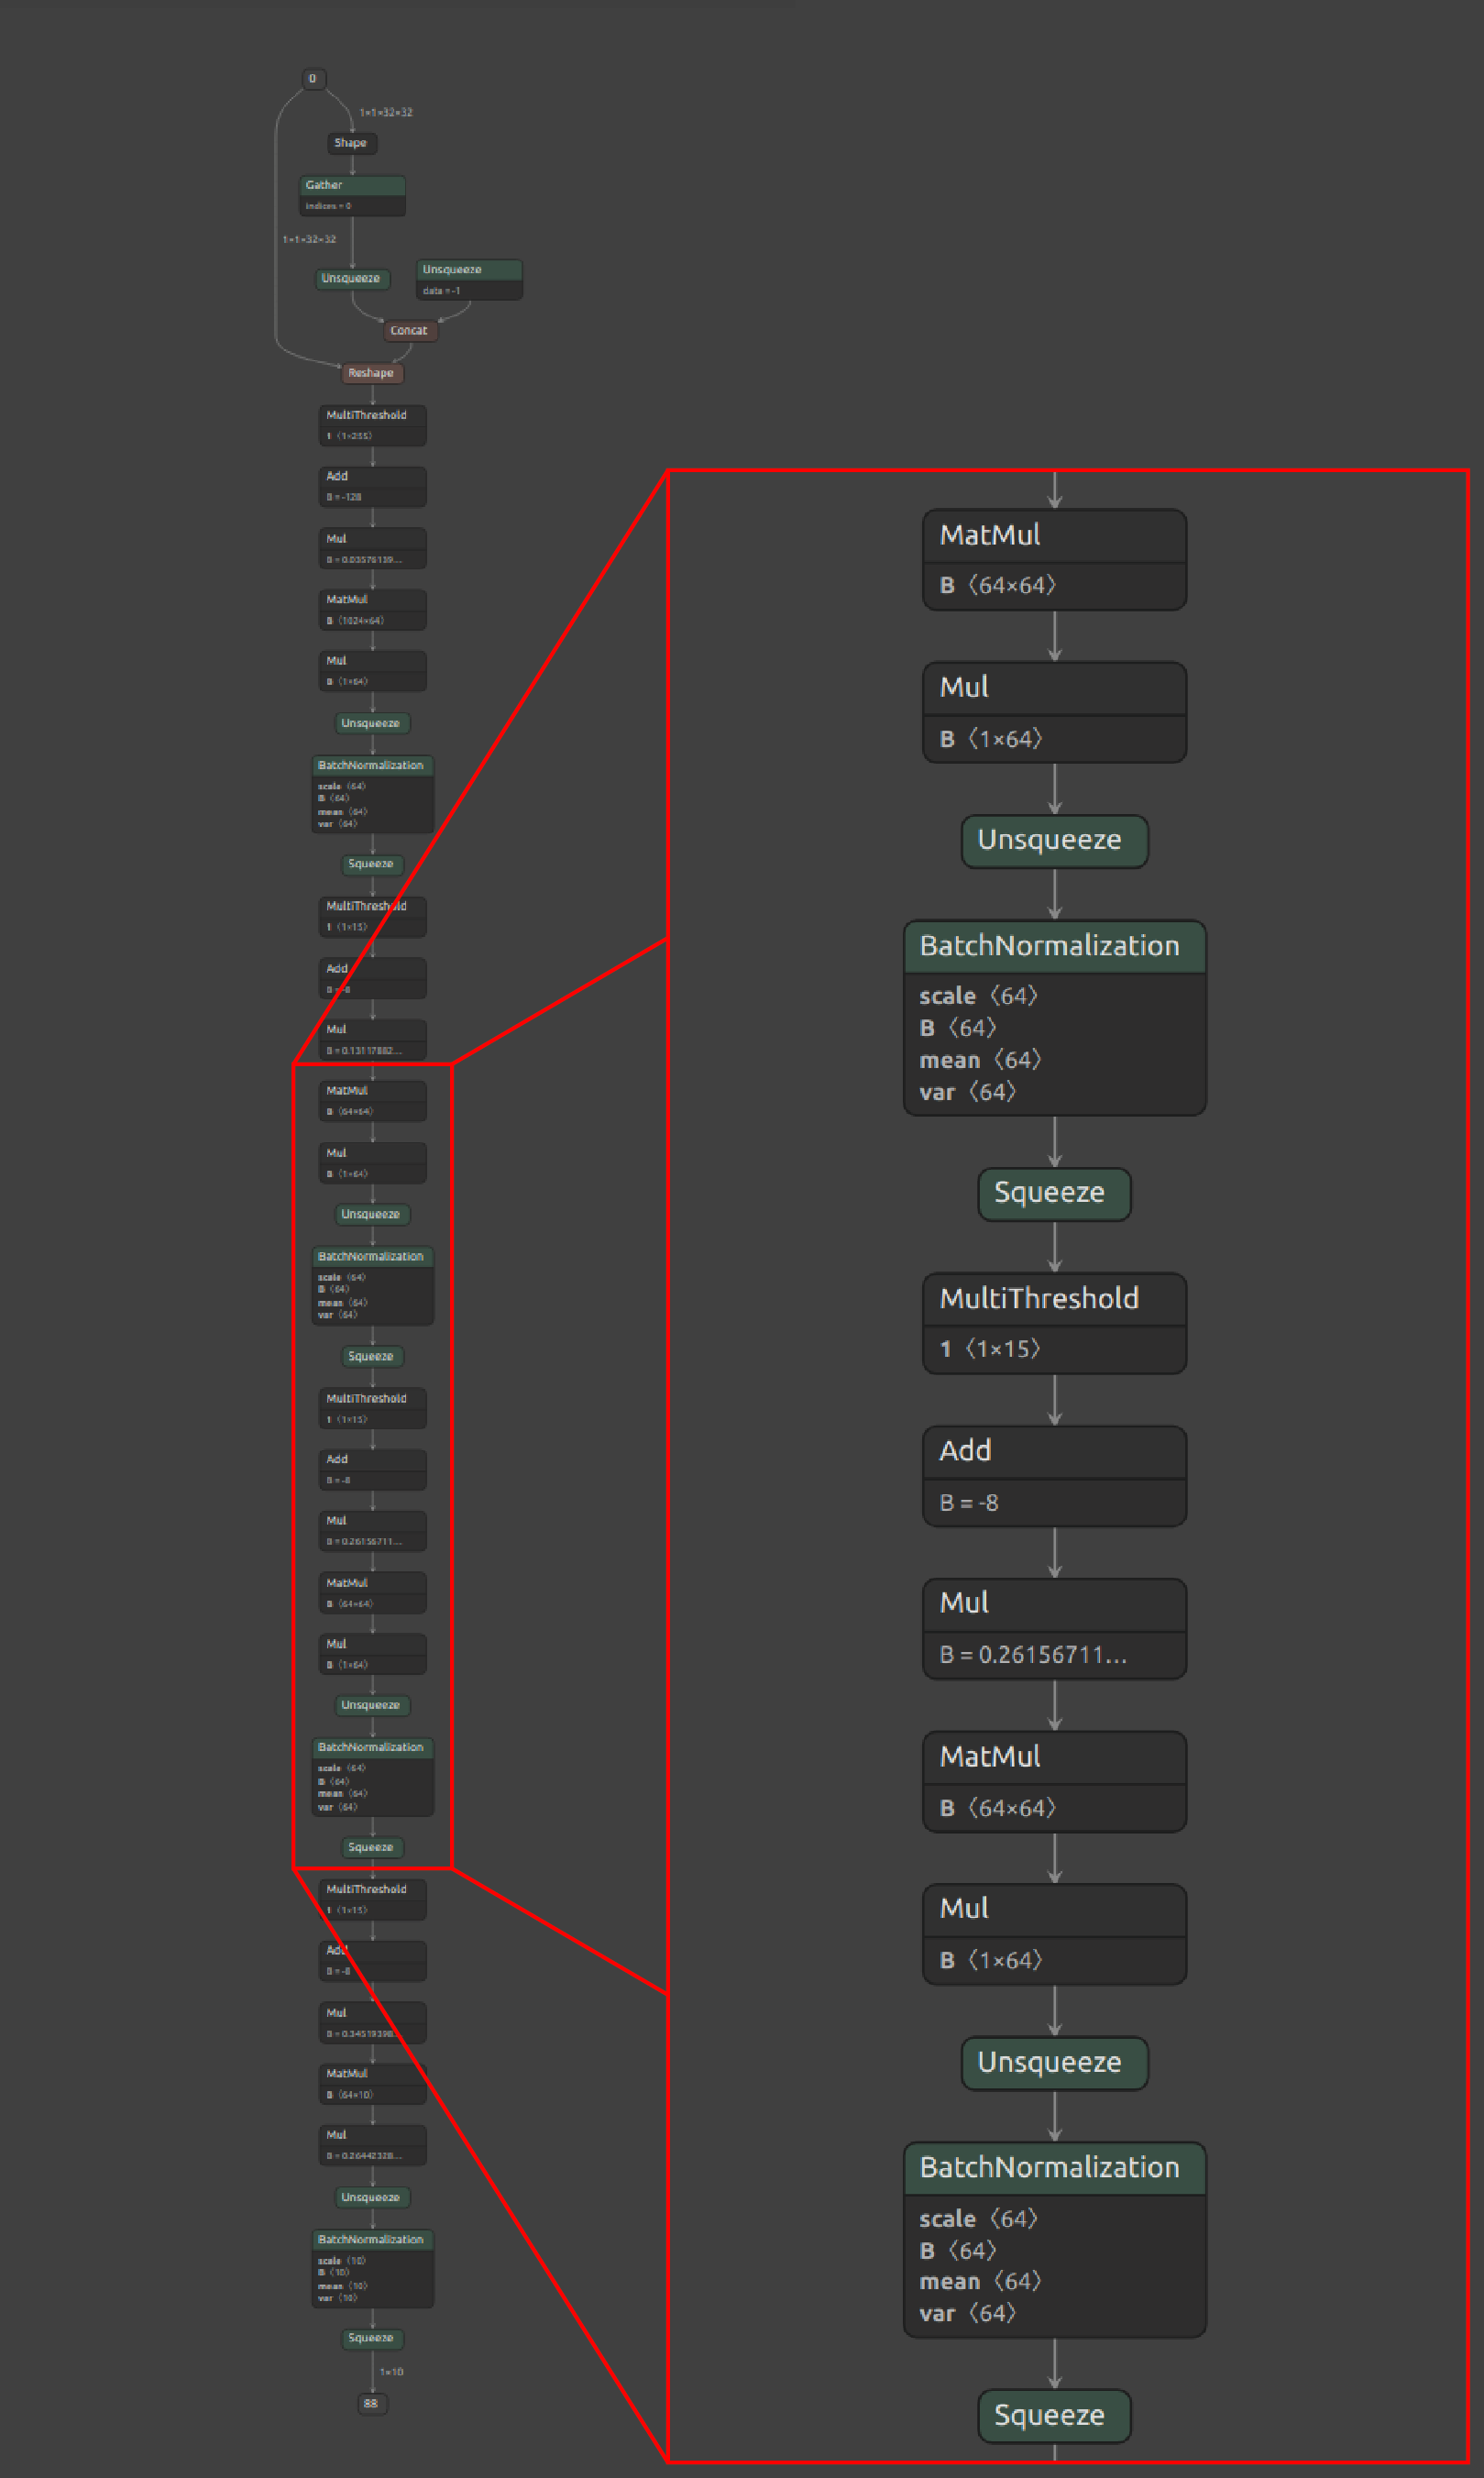
\includegraphics[width=12cm]{Figures/ONNXBeginning.png}
	\caption[TFC \emph{ONNX} representation]{TFC \emph{ONNX} Representation}
	\label{fig:ONNXBeginning}
\end{figure}

\newpage

%-------------------------
%	SUBSECTION 6.2.3 - FINN
%-------------------------

\subsection{FINN}

The last piece of the workflow is \emph{FINN}, described by Xilinx as allowing \guille{Fast, Scalable Quantized Neural Network Inference on FPGAs}. The \emph{FINN} compiler goes through three major steps to be able to port a neural network as shown on \emph{Figure} \ref{fig:FINNWholeFlow}. First, \emph{Network Preparation} where \emph{FINN} uses different transformations on the \emph{ONNX} graph to simplify it or make it more convenient for the next steps. Then, \emph{IP Generation} where the \emph{Vivado} tool is called to generate a network of HLS layers with one IP block per layer and finally stitches all the blocks together. Finally, the network is deployed on an FPGA with a \emph{PYNQ} shell, an FPGA utility providing a Python environment on an FPGA. This deployment is made possible by creating a project and driver then transferring it on the board along with the bitfile.

% \emph{FINN} WHOLE FLOW
\begin{figure}[htbp]
	\centering
		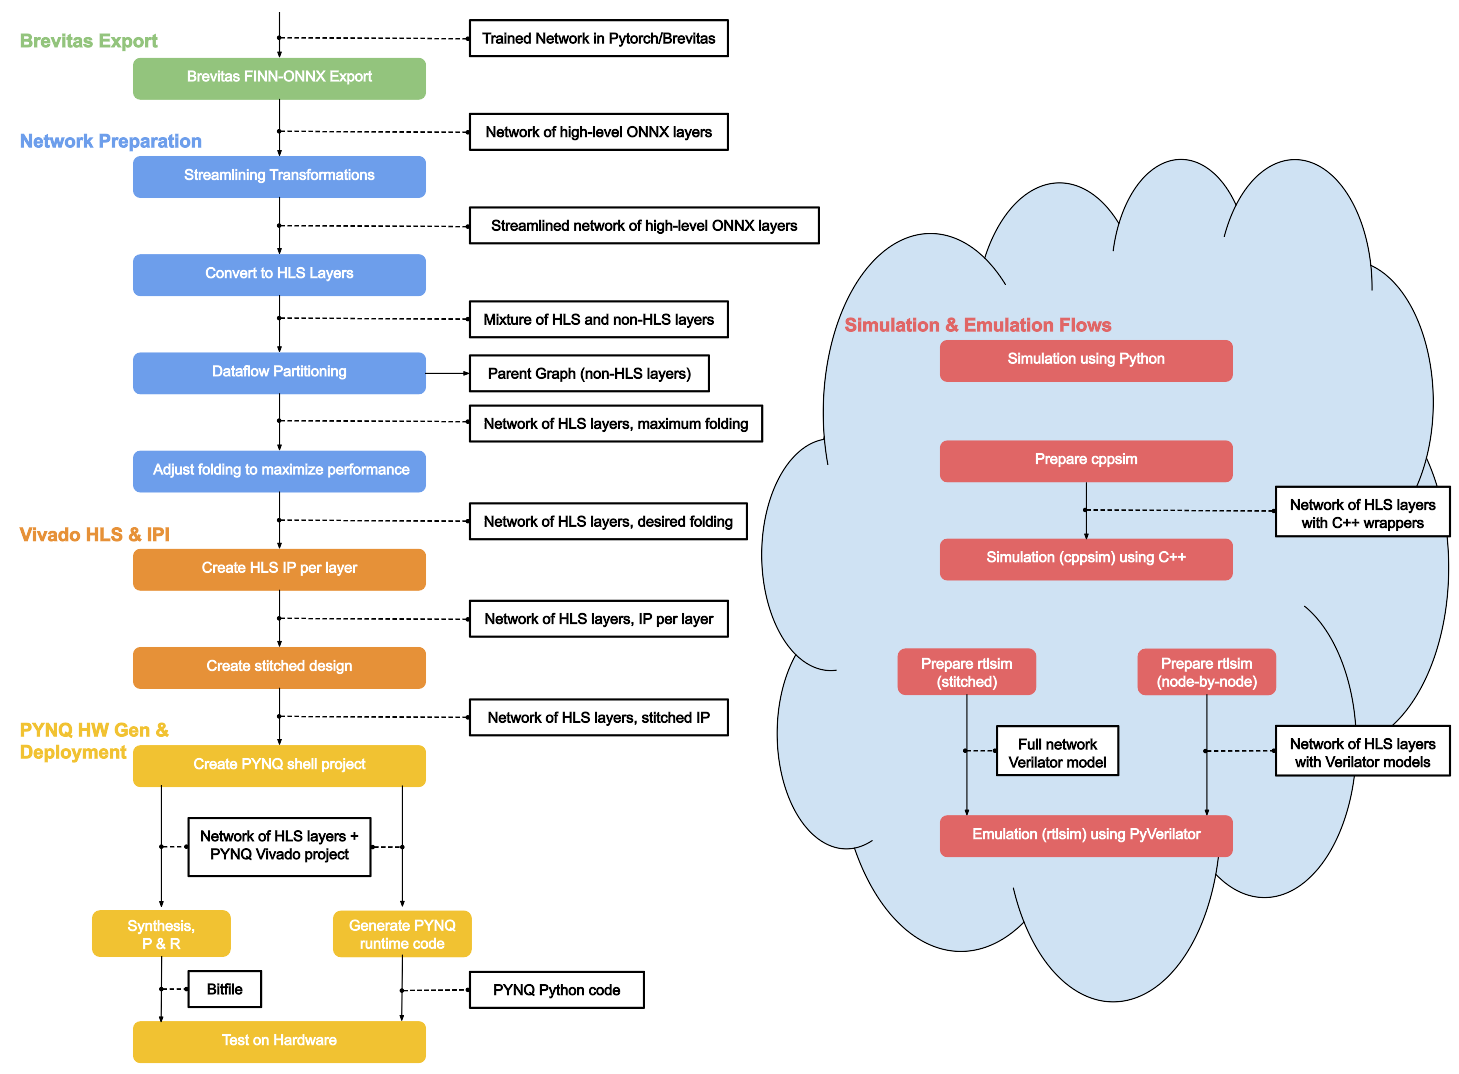
\includegraphics[width=16cm]{Figures/FINNWholeFlow.png}
	\caption[FINN whole flow]{FINN workflow from \emph{Brevitas} import to FPGA deployment}
	\label{fig:FINNWholeFlow}
\end{figure}

% \emph{FINN} TRANSFORMATIONS
\begin{figure}[htbp]
	\centering
		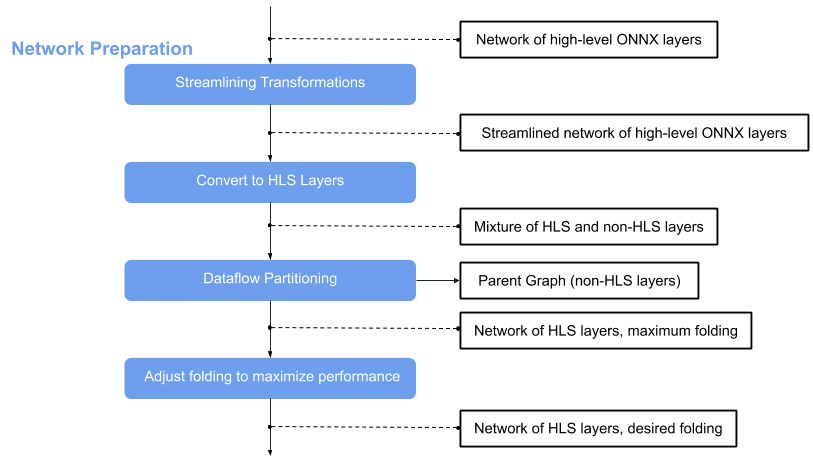
\includegraphics[width=10cm]{Figures/FINNTransformations.png}
	\caption[FINN Transformations]{FINN Transformations}
	\label{fig:FINNTransformations}
\end{figure}

The network preparation part is the one involving several transformations in the structure of the neural network graph. The transformations are separated in three categories: tidy-up, streamlining, HLS conversion and dataflow partition. All the different transformations, whether they are used for tidy-up or synthesis purposes, are applied on a \texttt{ModelWrapper}. The flow of transformations can be seen on \emph{Figure} \ref{fig:FINNTransformations}.

\emph{Tidy-up Transformations} consist of renaming the nodes so they have unique names, checking the data type and shapes of the tensors used. Examples of these different transformations are \texttt{GiveReadableTensorNames}, \texttt{GiveUniqueNodeNames} or \texttt{InferShapes}.

\emph{Streamline Transformations} consist of a way to remove floating-point operations from the graph. The streamlining process itself contains three steps:
\begin{itemize}
  \item \textbf{Successive Thresholding}: Given a set of threshold values, the successive thresholding function maps any real number $x$ to an integer corresponding to the number of thresholds $x$ is greater or equal to. This way, any uniform quantifier can be expressed as successive thresholding followed by a linear transformation: $Q(x) = a*T(x) + b$.
  \item \textbf{Collapsing Linear Transformation}: All \emph{floating point} linear operations are positioned between the quantised matrix operation and the activation quantisation. Any sequence of linear transformation can be collapsed in a single linear transformation.
  \item \textbf{Absorbing into Thresholds} :Updating the threshold values with the changes in the linear transformations removes any linear transformation from the graph.
\end{itemize}

The \texttt{Streamline} transformation class is implemented as presented on \emph{Listing} \ref{fig:FINNStreamline}.

\begin{mylisting}[htbp]
\centering
\begin{lstlisting}[language=Python]
class Streamline(Transformation):
  """Apply the streamlining transform, see arXiv:1709.04060."""

  def apply(self, model):
    streamline_transformations = [
      ConvertSubToAdd(),
      ConvertDivToMul(),
      BatchNormToAffine(),
      ConvertSignToThres(),
      MoveAddPastMul(),
      MoveScalarAddPastMatMul(),
      MoveScalarAddPastConv(),
      MoveScalarMulPastMatMul(),
      MoveScalarMulPastConv(),
      MoveAddPastMul(),
      CollapseRepeatedAdd(),
      CollapseRepeatedMul(),
      AbsorbAddIntoMultiThreshold(),
      FactorOutMulSignMagnitude(),
      AbsorbMulIntoMultiThreshold(),
      Absorb1BitMulIntoMatMul(),
      Absorb1BitMulIntoConv(),
      RoundAndClipThresholds(),
    ]
    for trn in streamline_transformations:
      model = model.transform(trn)
      model = model.transform(GiveUniqueNodeNames())
      model = model.transform(GiveReadableTensorNames())
      model = model.transform(InferDataTypes())
    return (model, False)
\end{lstlisting}
\caption[FINN Streamline]{FINN Streamline process as proposed in \cite{Umuroglu2017b, Blott2018}}
	\label{fig:FINNStreamline}
\end{mylisting}

\newpage

Once the streamlining transformations are completed, \emph{FINN} will convert the different layers to their HLS counterpart if possible. This conversion is made possible by using \texttt{finn-hls}, a backend library developed by the same team to translate layers to HLS. The result of the transformation consists of a mixture of HLS and non-HLS layers. The \emph{HLS Conversion} completed, \emph{FINN} will then proceed to a \emph{Dataflow Partitioning}. This step will separate the whole network graph into a parent graph that will be executed through the \texttt{onnx-exec}. One of its child node contains all the different HLS layers and during the execution of the whole graph, \emph{FINN} delegates the execution of this child node to the FPGA board and gets the result before injecting it back in the graph execution flow. The resulting \emph{ONNX} representation can be seen on \emph{Figure} \ref{fig:ONNXEnd} where the network and its \emph{ONNX} representation (presented earlier on \emph{Figure} \ref{fig:ONNXBeginning}) now corresponds to few basic operations followed by a \texttt{StreamingDataflowPartition} layer that contains the layers that need to be deployed.

\newpage

% END TFC \emph{ONNX} THROUGH NETRON
\begin{figure}[htbp]
	\centering
		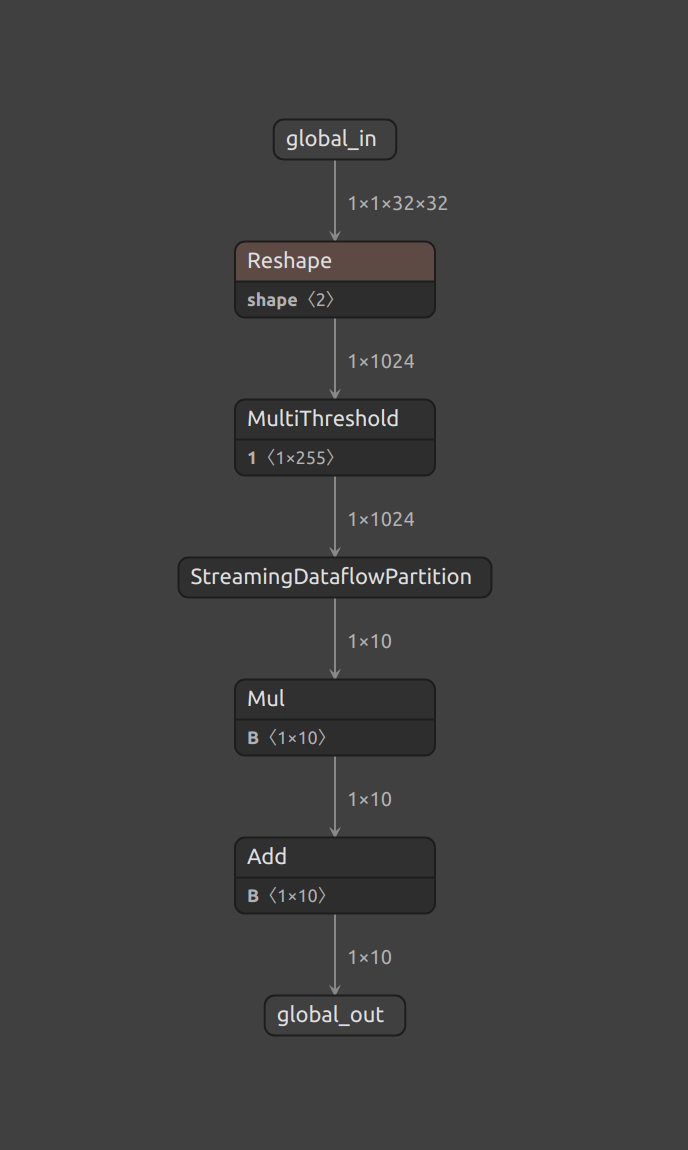
\includegraphics[width=6cm]{Figures/ONNXEnd.png}
	\caption[Transformed TFC \emph{ONNX} representation]{Transformed TFC \emph{ONNX} Representation}
	\label{fig:ONNXEnd}
\end{figure}

Once the graph is separated into two distinct parts, the synthesis can begin using \emph{Vivado}. Each layer is converted to one \emph{IP block}, a logical unit, then they are all stitched together to form the whole partition that will be ported to the board, as presented on \emph{Figure} \ref{fig:FINNSynthesis}. This part produces a \emph{bitfile} that defines the configuration of the FPGA.

% \emph{FINN} SYNTHESIS
\begin{figure}[htbp]
	\centering
		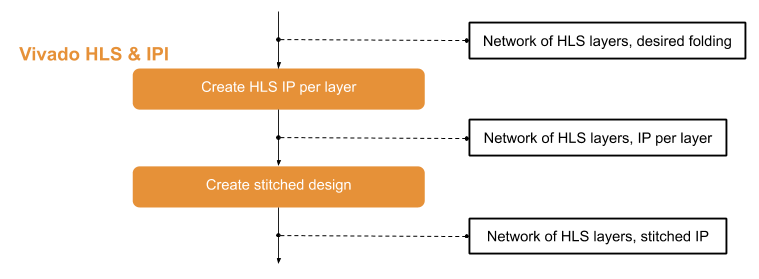
\includegraphics[width=10cm]{Figures/FINNSynthesis.png}
	\caption[FINN Synthesis]{FINN Synthesis}
	\label{fig:FINNSynthesis}
\end{figure}

Finally, the default built-in way to deploy the bitfile and execute it is to use the Python shield image named \emph{PYNQ}. This shield provides a Python environment to interact with the board. \emph{FINN} therefore creates and deploys a PYNQ project that consists of the base modules needed, a project structure and a simple driver. Once the project bitfile is transferred on the board, the driver can feed it with the image to inference, collect the result and send it back to the \texttt{onnx-exec} process. These different parts are summarised on \emph{Figure} \ref{fig:FINNPYNQ}.

% PYNQ DEPLOYMENT
\begin{figure}[htbp]
	\centering
		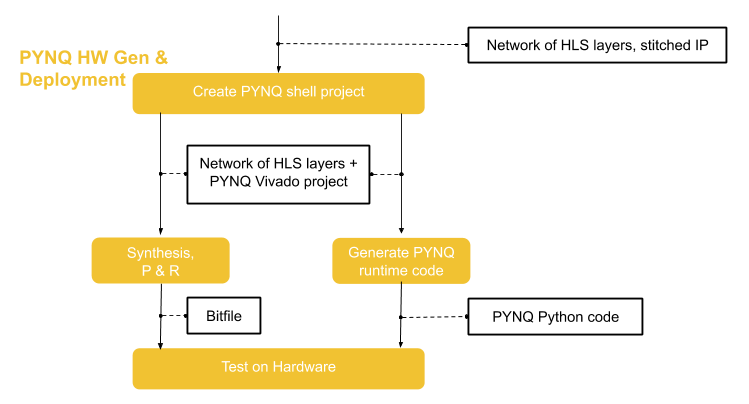
\includegraphics[width=10cm]{Figures/FINNPYNQ.png}
	\caption[FINN PYNQ Deployment]{FINN PYNQ Deployment}
	\label{fig:FINNPYNQ}
\end{figure}

%-------------------------------------------
%	SUBSECTION 6.2.4 - Benchmark as extension
%-------------------------------------------

\subsection{Benchmark as Extension}

The workflow \emph{Brevitas} / \emph{ONNX} / \emph{FINN} presents an interesting straightforward way to port a neural network on an FPGA board. In order to design a benchmark of the framework and to assess the impact of quantisation, there is a need for another layer on top of \emph{Brevitas} that should be able to train, evaluate and export neural networks. While Xilinx developers provide several examples to train and export different networks, they do not respect a common API nor the same structure rules. They are bundled in separate projects with instructions on how to run the training again but no insight is provided on what do hardcoded values mean on several quantised layers.

The different objectives of the benchmark are:
\begin{itemize}
  \item Present a common API to train neural networks, quantised or not.
  \item Be able to resume the training at any point.
  \item Log the different parts of the training.
  \item Define well-known neural networks and their quantised counterparts.
  \item Set an easy access to well-known datasets.
  \item Provide a common API to evaluate neural networks.
  \item Be able to export the trained neural network to \emph{ONNX}.
\end{itemize}

The project is structured as follows:
\begin{itemize}
  \item \textbf{\texttt{core}}: Core functionalities of the benchmark tool. This sub-package contains the \texttt{CLI}, \texttt{Trainer}, \texttt{Plotter}, \texttt{Logger} and \texttt{Exporter}. The \texttt{Trainer} is the main piece and is given all the arguments passed to the \texttt{CLI}. The \texttt{Logger} logs training routine, the \texttt{Plotter} allows to visualise instances of the dataset and the \texttt{Exporter} performs the export to \emph{ONNX}.
  \item \textbf{\texttt{extensions}}: Extensions of PyTorch functionalities to perform with quantised networks. These extensions consist of a new dataset, \emph{GTSRB}, a new loss function that can be used with binary networks, \emph{Squared Hinge Loss}, and a helper layer that performs the norm of the tensor.
  \item \textbf{\texttt{networks}}: Network architectures and their quantised counterpart. The defined networks consist of \texttt{TFC} ()three \emph{FC} layers next to each other), \texttt{CNV} (a simple CNN), \texttt{LeNet5}, \texttt{VGG11}, \texttt{VGG13}, \texttt{VGG16}, \texttt{VGG19} and \texttt{MobilenetV1}. All the different architectures answer to the same API and can be created by passing the number of \emph{classes}, number of \emph{in-channels} and the different quantisations if using a quantised network. The creation of a simple network and its quantised counterpart can be seen on \emph{Listing} \ref{fig:NetworkCreation}.
\end{itemize}

% PROJECT UML
% \begin{figure}[htbp]
% 	\centering
% 		\includegraphics[width=8cm]{Figures/BenchCLI.png}
% 	\caption[Benchmark CLI]{Benchmark Command Line Interface}
% 	\label{fig:BenchCLI}
% \end{figure}


\begin{mylisting}[htbp]
\centering
\begin{lstlisting}[language=Python]
from nn_benchmark.networks import LeNet5, QuantLeNet5

# To train a classic PyTorch network on MNIST for example
# (10 classes and black and white images)
lenet5 = LeNet5(n_classes = 10, in_channels = 1)

# To train a quantised \emph{Brevitas} network on CIFAR-10 for example
# (10 classes and RGB images) with quantisations of 2 bits for the
# weights, 2 bits for the activations and 4 bits for the first layer
quant_lenet5 = QuantLeNet5(n_classes = 10, in_channels = 3,
                           weight_bit_width = 2,
                           act_bit_width    = 2,
                           in_bit_width     = 4)
\end{lstlisting}
\caption[NetworkCreation]{Network Creation with the benchmark tool}
	\label{fig:NetworkCreation}
\end{mylisting}

The training routine is wrapped up by the \texttt{Trainer} class and can be tuned through the command line. The \texttt{CLI} class holds a large number of parameters that can be used to customise the training phase. An example of a run can be seen on \emph{Figure} \ref{fig:BenchCLI}. The example presented on the figure will launch the training for the network \texttt{QuantTFC}, the \emph{Brevitas} version of the \emph{TFC} network (three successive fully-connected layers). This training will be run on the \texttt{FashionMNIST} dataset for 100 epochs. It will be overlooked by the \texttt{ADAM} optimiser and \texttt{CrossEntropy} loss function. The hyper-parameters are tuned to a learning rate of 0.01 and a momentum of 0.9. The learning rate will change according to the scheduler, here a \texttt{MultiStepScheduler}. This scheduler will divide by 10 the learning rate after the epochs specified as milestones, here 34 and 37. Finally, the \emph{activation quantisation} is set to 2 bit, same for the \emph{weight quantisation} and the \emph{input quantisation} is set to 8 bits. The input quantisation is used for the first layer only. This often outputs better results due to the avoided harsh precision reduction. The first layers impact end accuracy a lot more than the last ones and the quantisation has to be delayed.

\begin{mylisting}[htbp]
\centering
\begin{lstlisting}[language=bash]
PYTORCH_JIT=1 python nn_benchmark/main.py \
--network    QuantTFC     \
--dataset    FashionMNIST \
--epochs     100          \
--optimiser  ADAM         \
--loss       CrossEntropy \
--lr         0.01         \
--momentum   0.9          \
--scheduler  STEP         \
--milestones 34,37        \
--acq        2            \
--weq        2            \
--inq        8
\end{lstlisting}
\caption[Command Line Interface]{Command Line Interface arguments}
	\label{fig:BenchCLI}
\end{mylisting}

The programs in \texttt{quant\_utils\/} present helper methods to create the different quantised layers. Those helpers work as both a simplification of the quantised layers API but also as controllers of the homogeneity of the layers functionalities. This homogeneity is crucial as, for now, \emph{FINN} can only handle a subset of what \emph{Brevitas} is able to design and train.

The final project can be seen on GitHub under the name \texttt{nn\_benchmark} \cite{BenchmarkRepo}.

%----------------------------------------------------------------------------------------
%	SECTION 6.3 - Methodology and Setup
%----------------------------------------------------------------------------------------

\section{Methodology and Setup}

This section will present the setup and methodology of the different experiments run. This is important for reproducibility purposes and to present results comparable to the literature. Those results aim at being extended in the future. \emph{FINN} and \emph{Brevitas} are not released yet and are still in development. The API of both tools is subject to change and results will need to be reassessed. However, the training part of the benchmark should not be subject to change as it uses a subset of the \emph{Brevitas} functionalities. While \emph{Brevitas} allows extensive tuning and customisation of both networks and training routine, \emph{FINN} can only (for now) handle a subset of those customisations.

%-----------------------------------
%	SUBSECTION 6.3.1 - Experiments
%-----------------------------------

\subsection{Experiments}

In order to assess the impact of quantisation, the objective is to deploy a neural network with varying precision for its weights and activations. The different metrics that will be taken in consideration are the following:

\begin{itemize}
  \item \textbf{Weight Bitwidth}: The number of bits in the weight precision.
  \item \textbf{Activation Bitwidth}: The number of bits in the activation precision.
  \item \textbf{Network Accuracy}: The final accuracy of the trained network on the test set.
  \item \textbf{Training Time}: Number of epochs the network was trained for.
  \item \textbf{Hardware Utilisation}: Look-up tables (LUT), flip-flops (FF) and BRAM usage.
  \item \textbf{Throughput}: Number of image the deployed network can process per second.
\end{itemize}

The initial objective was to train three different neural networks and their according datasets, the three being:
\begin{itemize}
  \item \textbf{TFC} for \textbf{Fashion-MNIST}: A simple neural network containing three fully-connected layers to train on a variation of the handwritten digits dataset, \emph{Fashion-MNIST} using small grayscale images of garments.
  \item \textbf{CNV} for \textbf{CIFAR-10}: A simple convolutional neural network to run on a classic 3-channels dataset, CIFAR-10.
  \item \textbf{MobilenetV1} for \textbf{GTSRB}: This network is interesting due to the fact it has been designed with portability in mind, coupling it with a street signs dataset makes it an interesting combination in an autonomous driving context.
\end{itemize}

%--------------------------------------
%	SUBSECTION 6.3.2 - Training
%--------------------------------------

\subsection{Training}

The training of the different networks is made with the following parameters and hyper-parameters:
\begin{itemize}
  \item \textbf{Epochs}: 40
  \item \textbf{Momentum}: 0.9
  \item \textbf{Learning Rate}: 0.01
  \item \textbf{Scheduler}: Multi-step scheduler, the learning rate is divided by 10 on epochs 34 and 37 as done in \cite{Bethge2018}.
  \item \textbf{Batch size}: 100 instances per batch.
  \item \textbf{Loss function}: The loss function used is \emph{Cross Entropy}.
  \item \textbf{Optimiser}: The optimiser use dis the \emph{ADAM} optimiser as it has been shown it is the most performing one when dealing with reduced precision \cite{Alizadeh2018}.
\end{itemize}

Along with those parameters, the bit-widths of weights and activations are taken from 2 to 32 bits. There are no differences here between the weights and activations. While \cite{Bacchus2020} differentiates the bit-widths, this functionality is still not fully supported in \emph{Brevitas} / \emph{FINN}. The inputs are either 8 bits (for sub-8bits weights and activations) or 32 bits (for 16 and 32-bits weights and activations). Using higher inputs (precision of the first layer) will help not deteriorate the end accuracy too much. A summary of the bit-widths used follows:
\begin{itemize}
  \item \textbf{weights}: 2, 4, 8, 16, 32
  \item \textbf{activations}: 2, 4, 8, 16, 32
  \item \textbf{inputs}: 8, 8, 8, 32, 32
\end{itemize}

Rather than using the \emph{CLI} to specify the training configuration for each one of the neural networks as in \emph{Listing} \ref{fig:BenchCLI}, a running script is provided as presented in \emph{Listing} \ref{fig:TrainingScript}. This script emulates the \emph{CLI} by passing the specified parameters and hyper-parameters presented earlier but varying both the network architecture, dataset and the different bit-widths.

\begin{mylisting}[htbp]
\centering
\begin{lstlisting}[language=Python]
import sys
from nn_benchmark.core import ObjDict, Trainer
from nn_benchmark.networks import QuantTFC, QuantCNV, QuantMobilenetV1

if __name__ == "__main__":
    acq_list = [2, 4, 8, 16, 32]
    weq_list = [2, 4, 8, 16, 32]
    inq_list = [8, 8, 8, 32, 32]

    args = {'datadir': './data/', 'experiments': './experiments', 'dry_run': False,
            'log_freq': 10, 'evaluate': False, 'resume': None, 'detect_nan': False,
            'num_workers': 4, 'gpus': '0', 'batch_size': 100, 'lr': 0.01, 'optim': 'ADAM',
            'loss': 'CrossEntropy', 'scheduler': 'STEP', 'milestones': '34,37',
            'momentum': 0.9, 'weight_decay': 0, 'epochs': 40, 'random_seed': 1,
            'network': None, 'pretrained': False, 'dataset': None,
            'visualize': False, 'acq': None, 'weq': None, 'inq': None, 'onnx': False}
    args = ObjDict(args)

    # QuantTFC on Fashion-MNIST
    args.network = "QuantTFC"
    args.dataset = "FASHION-MNIST"
    for acq, weq, inq in zip(acq_list, weq_list, inq_list):
        args.acq = acq
        args.weq = weq
        args.inq = inq
        trainer_tfc = Trainer(args)
        trainer_tfc.train_model()

    # QuantCNV on CIFAR-10
    args.network = "QuantCNV"
    args.dataset = "CIFAR10"
    for acq, weq, inq in zip(acq_list, weq_list, inq_list):
        args.acq = acq
        args.weq = weq
        args.inq = inq
        trainer_cnv = Trainer(args)
        trainer_cnv.train_model()

    # QuantMobilenetV1 on GTSRB
    args.network = "QuantMobilenetV1"
    args.dataset = "GTSRB"
    for acq, weq, inq in zip(acq_list, weq_list, inq_list):
        args.acq = acq
        args.weq = weq
        args.inq = inq
        trainer_mobilenet = Trainer(args)
        trainer_mobilenet.train_model()
\end{lstlisting}
\caption[Training Script]{Training Script to train all three networks}
	\label{fig:TrainingScript}
\end{mylisting}

%--------------------------------------
%	SUBSECTION 6.3.3 - Deployment
%--------------------------------------

\subsection{Deployment}

The deployment step is performed through the different \emph{FINN} transformations. The target architecture is a \emph{PYNQ-Z1}, a Python shell over a circuit from the \emph{Zynq} family. The \emph{Zynq} circuits are composed of an \guille{Ap SoC} (All Programmable System-on-Chip) that contains a dual-core ARM Cortex-A9.

While the target here is the base shell holder\emph{PYNQ-Z1}, the Python shell can be ported to other architectures. For now, the official supported architectures are \emph{PYNQ-Z1} or \emph{PYNQ-Z2} from Digilent and \emph{ZCU104} or \emph{ZCU111} from Xilinx. However, instructions to create your own image are available and several community \emph{PYNQ} images are available (\emph{Avnet Ultra96} for example).

Looking through the transformations steps presented earlier, here are the transformations used:
\begin{itemize}
  \item \textbf{Tidy-up}: This first step calls different transformations to simplify the graph. The transformations used here are \texttt{DoubleToSingleFloat}, \texttt{InferShapes}, \texttt{FoldConstants}, \texttt{GiveUniqueNodeNames}, \texttt{GiveReadableTensorNames} and \texttt{InferDataTypes}.
  \item \textbf{Streamline}: The streamline process described earlier is resumed to the \texttt{Streamline} transformation.
  \item \textbf{HLS Conversion}: The conversion consists of changing the layers to their HLS counterpart. In the case of quantised FC layers, the transformation is \texttt{Infer} \texttt{QuantizedStreamingFCLayer}.
  \item \textbf{Dataflow Partition}: The separation is contained in the \texttt{CreateDataflowParti-} \texttt{tion} transformation.
  \item \textbf{Folding}: The tuning operates on the child containing the HLS layers of the previously created partition. This folding is an empiric process for now but can be guided using \guille{folding factors}. Here, the folding factor used was 32. Each image consists of 1024 pixels ($32 \times 32$) and the PE and SIMD determines the number of simultaneous operations that can be processed in order to process the full image. The higher the folding factor, the higher number of passes are needed but the fewer hardware resources used. The \emph{PYNQ} being a relatively small FPGA, a folding factor of 16 was too much to handle and therefore 32 is chosen. The folding process can be seen on \emph{Listing} \ref{fig:FoldingProcess}. After selecting the PE and SIMD, the transformations \texttt{InsertDWC} \texttt{InsertFIFO} and \texttt{InsertTLastMarker} can be used.

  \begin{mylisting}[htbp]
  \centering
  \begin{lstlisting}[language=Python]
  fc_layers = model.get_nodes_by_op_type("StreamingFCLayer_Batch")
  # (PE, SIMD, in_fifo_depth, out_fifo_depth, ramstyle) for each layer
  # Test Divided by two the PE and in_fifo_depth
  config = [
      (16, 64, 16, 64, "block"),
      (8, 8, 64, 64, "auto"),
      (8, 8, 64, 64, "auto"),
      (10, 8, 64, 10, "distributed"),
  ]
  for fcl, (pe, simd, ififo, ofifo, ramstyle) in zip(fc_layers, config):
      fcl_inst = getCustomOp(fcl)
      fcl_inst.set_nodeattr("PE", pe)
      fcl_inst.set_nodeattr("SIMD", simd)
      fcl_inst.set_nodeattr("inFIFODepth", ififo)
      fcl_inst.set_nodeattr("outFIFODepth", ofifo)
      fcl_inst.set_nodeattr("ram_style", ramstyle)
  \end{lstlisting}
  \caption[Folding Process]{Folding process on the different layers}
  	\label{fig:FoldingProcess}
  \end{mylisting}
  \item \textbf{IP Synthesis}: The IP are synthesised using \texttt{PrepareIP}, \texttt{HLSSynthIP}, \texttt{ReplaceVeri-} \texttt{logRelPaths} and \texttt{CreateStitchedIP}. The result is a stitched IP consisting of one IP per layer succeeding one another. The resulting block design is presented on \emph{Figure} \ref{fig:StitchedBlockDesign} and displays successive \texttt{StreamingFIFO} and \texttt{StreamingFCLayer\_Batch}.

  \newpage

  % VIVADO STITCHED PROJECT
  \begin{figure}[htbp]
  	\centering
  		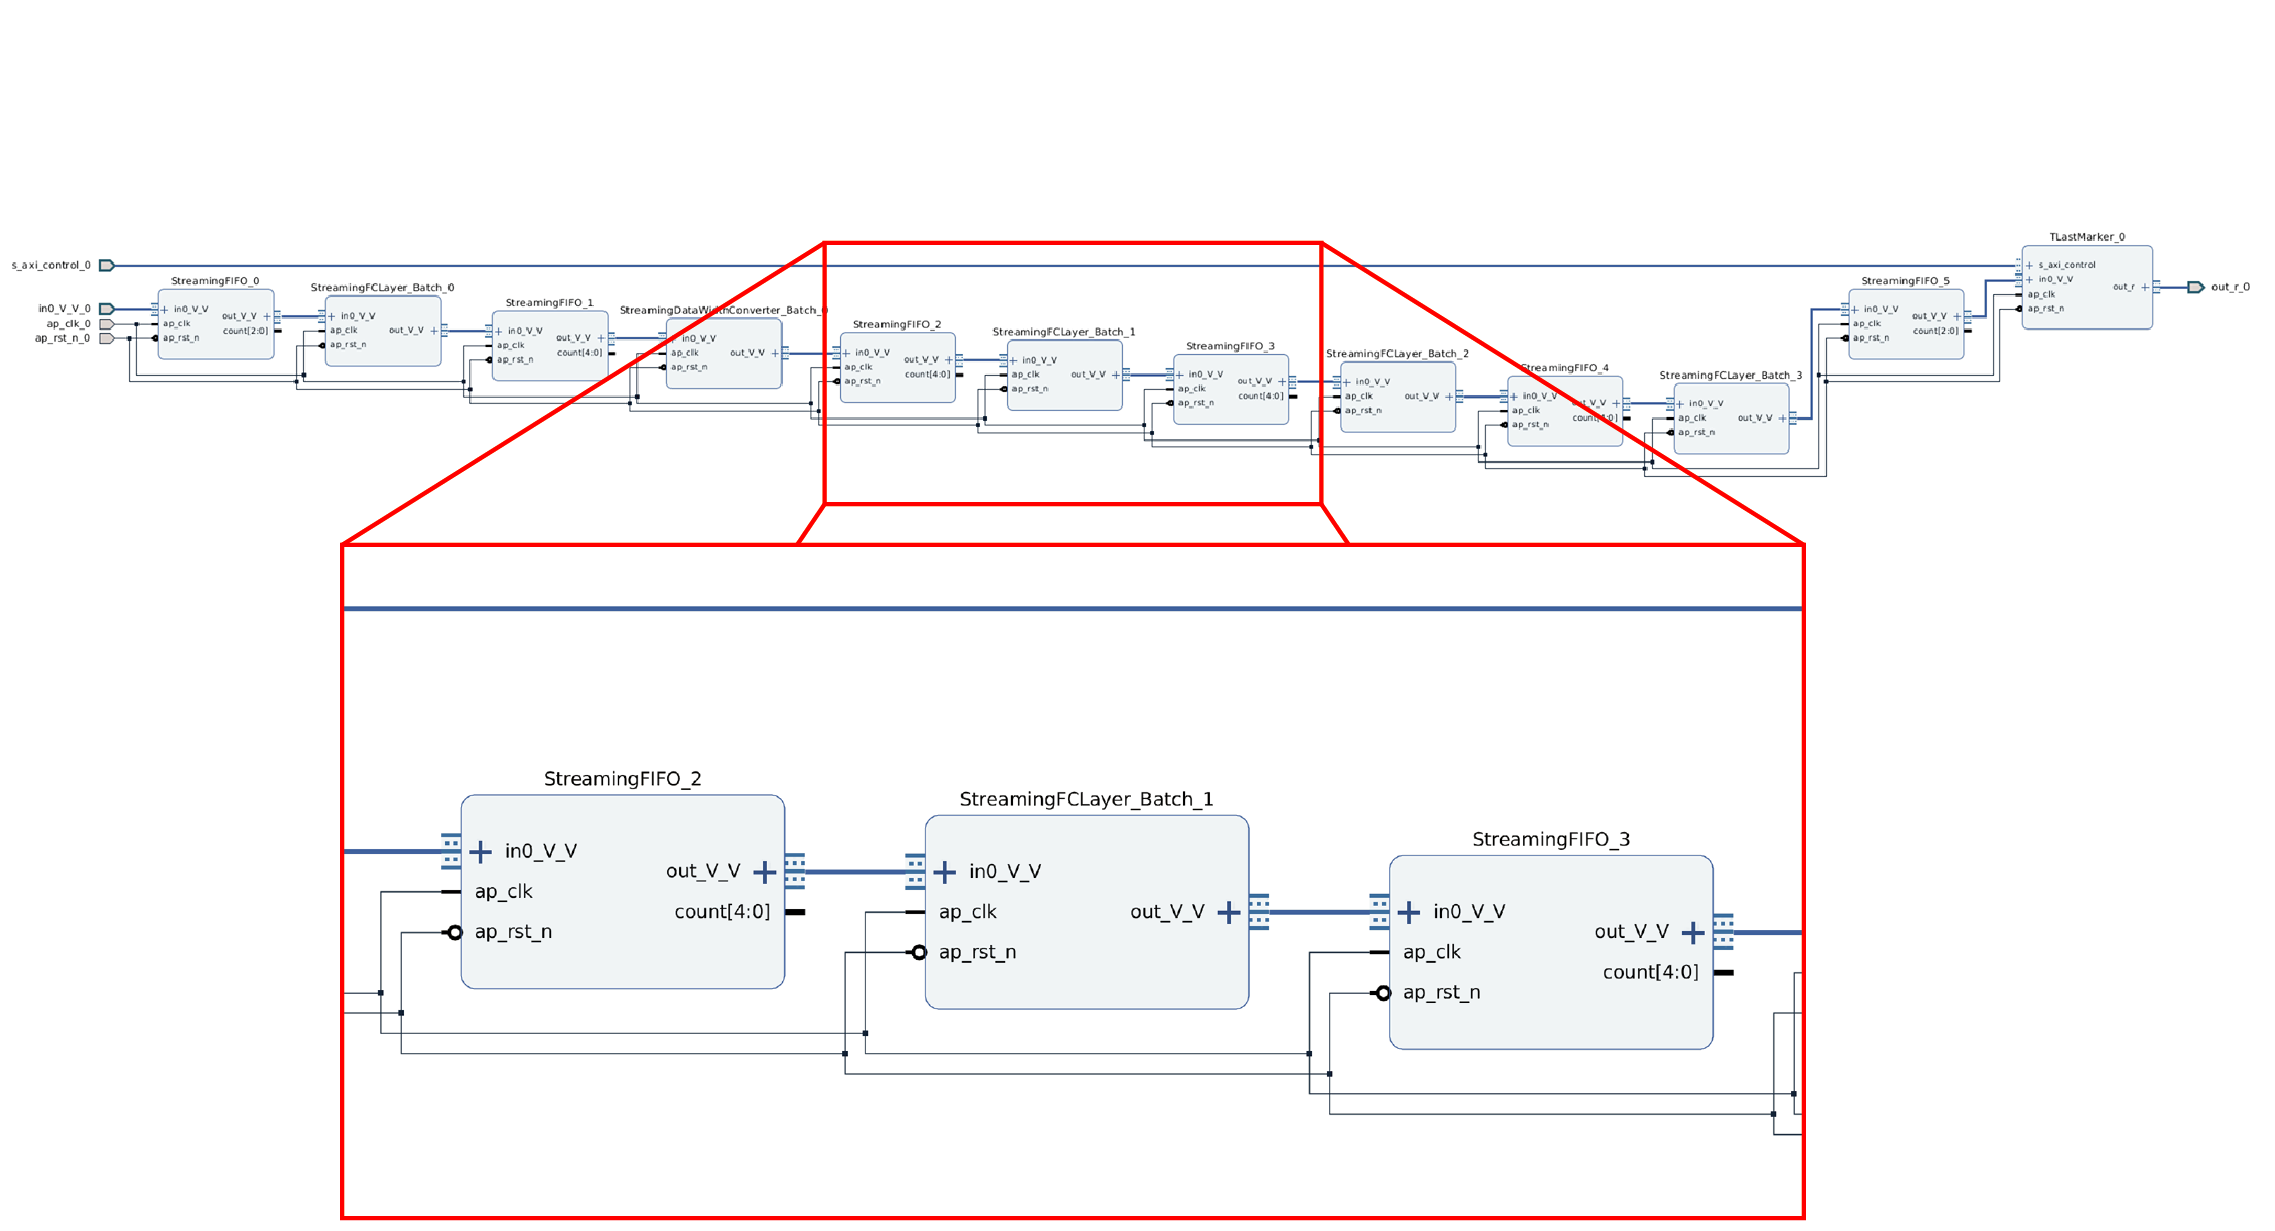
\includegraphics[width=\textwidth]{Figures/StitchedBlockDesign.png}
  	\caption[StitchedBlockDesign]{Block Design of the stitched IP layers}
  	\label{fig:StitchedBlockDesign}
  \end{figure}

  \item \textbf{PYNQ deployment}: The PYNQ driver and project are created with \texttt{Make-} \texttt{PYNQProject}, \texttt{SynthPYNQProject} and \texttt{MakePYNQDriver} and deployed with \texttt{DeployToPYNQ}.
\end{itemize}

These steps create a final \emph{Vivado} project, perform the synthesis and transfer the bitfile to the \emph{PYNQ-Z1}. An overview of the \emph{Vivado} block design can be seen on \emph{Figure} \ref{fig:ProjectBlockDesign}. The highlighted portion corresponds to the actual neural network part. The other components are links to the processing unit or external memory. A picture of the \emph{PYNQ-Z1} can be seen on \emph{Figure} \ref{fig:PYNQ-Z1}.

% FINAL VIVADO BLOCK DESIGN
\begin{figure}[htbp]
	\centering
		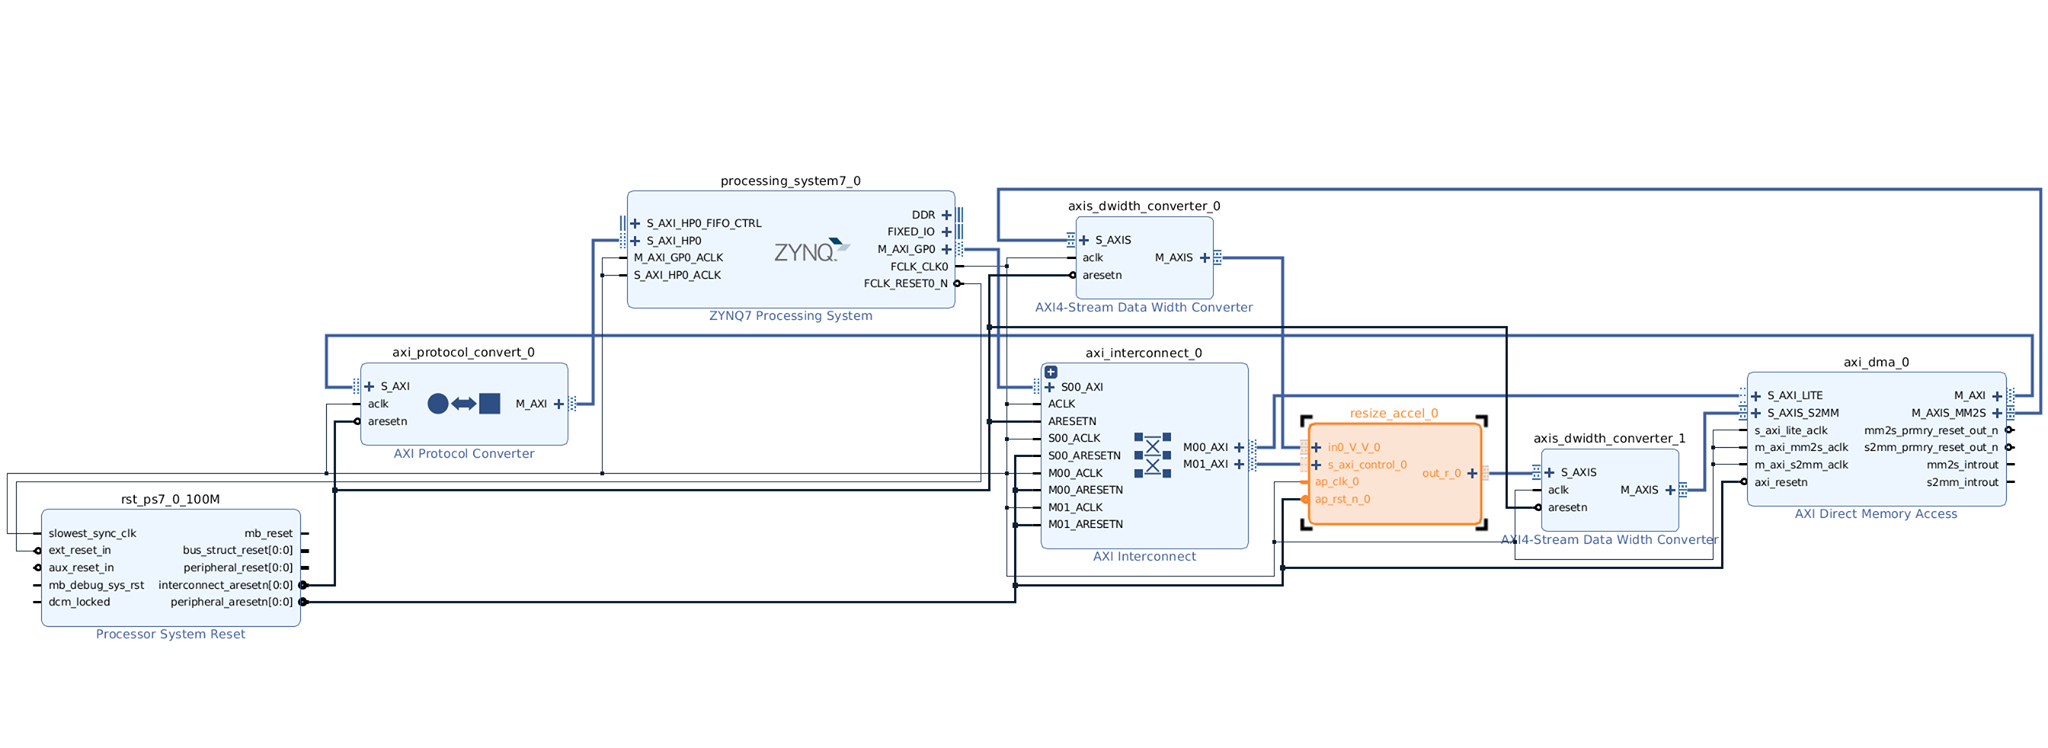
\includegraphics[width=\textwidth]{Figures/ProjectBlockDesign.png}
	\caption[ProjectBlockDesign]{Final Vivado Block Design}
	\label{fig:ProjectBlockDesign}
\end{figure}

% PYNQ PHOTO
\begin{figure}[htbp]
	\centering
		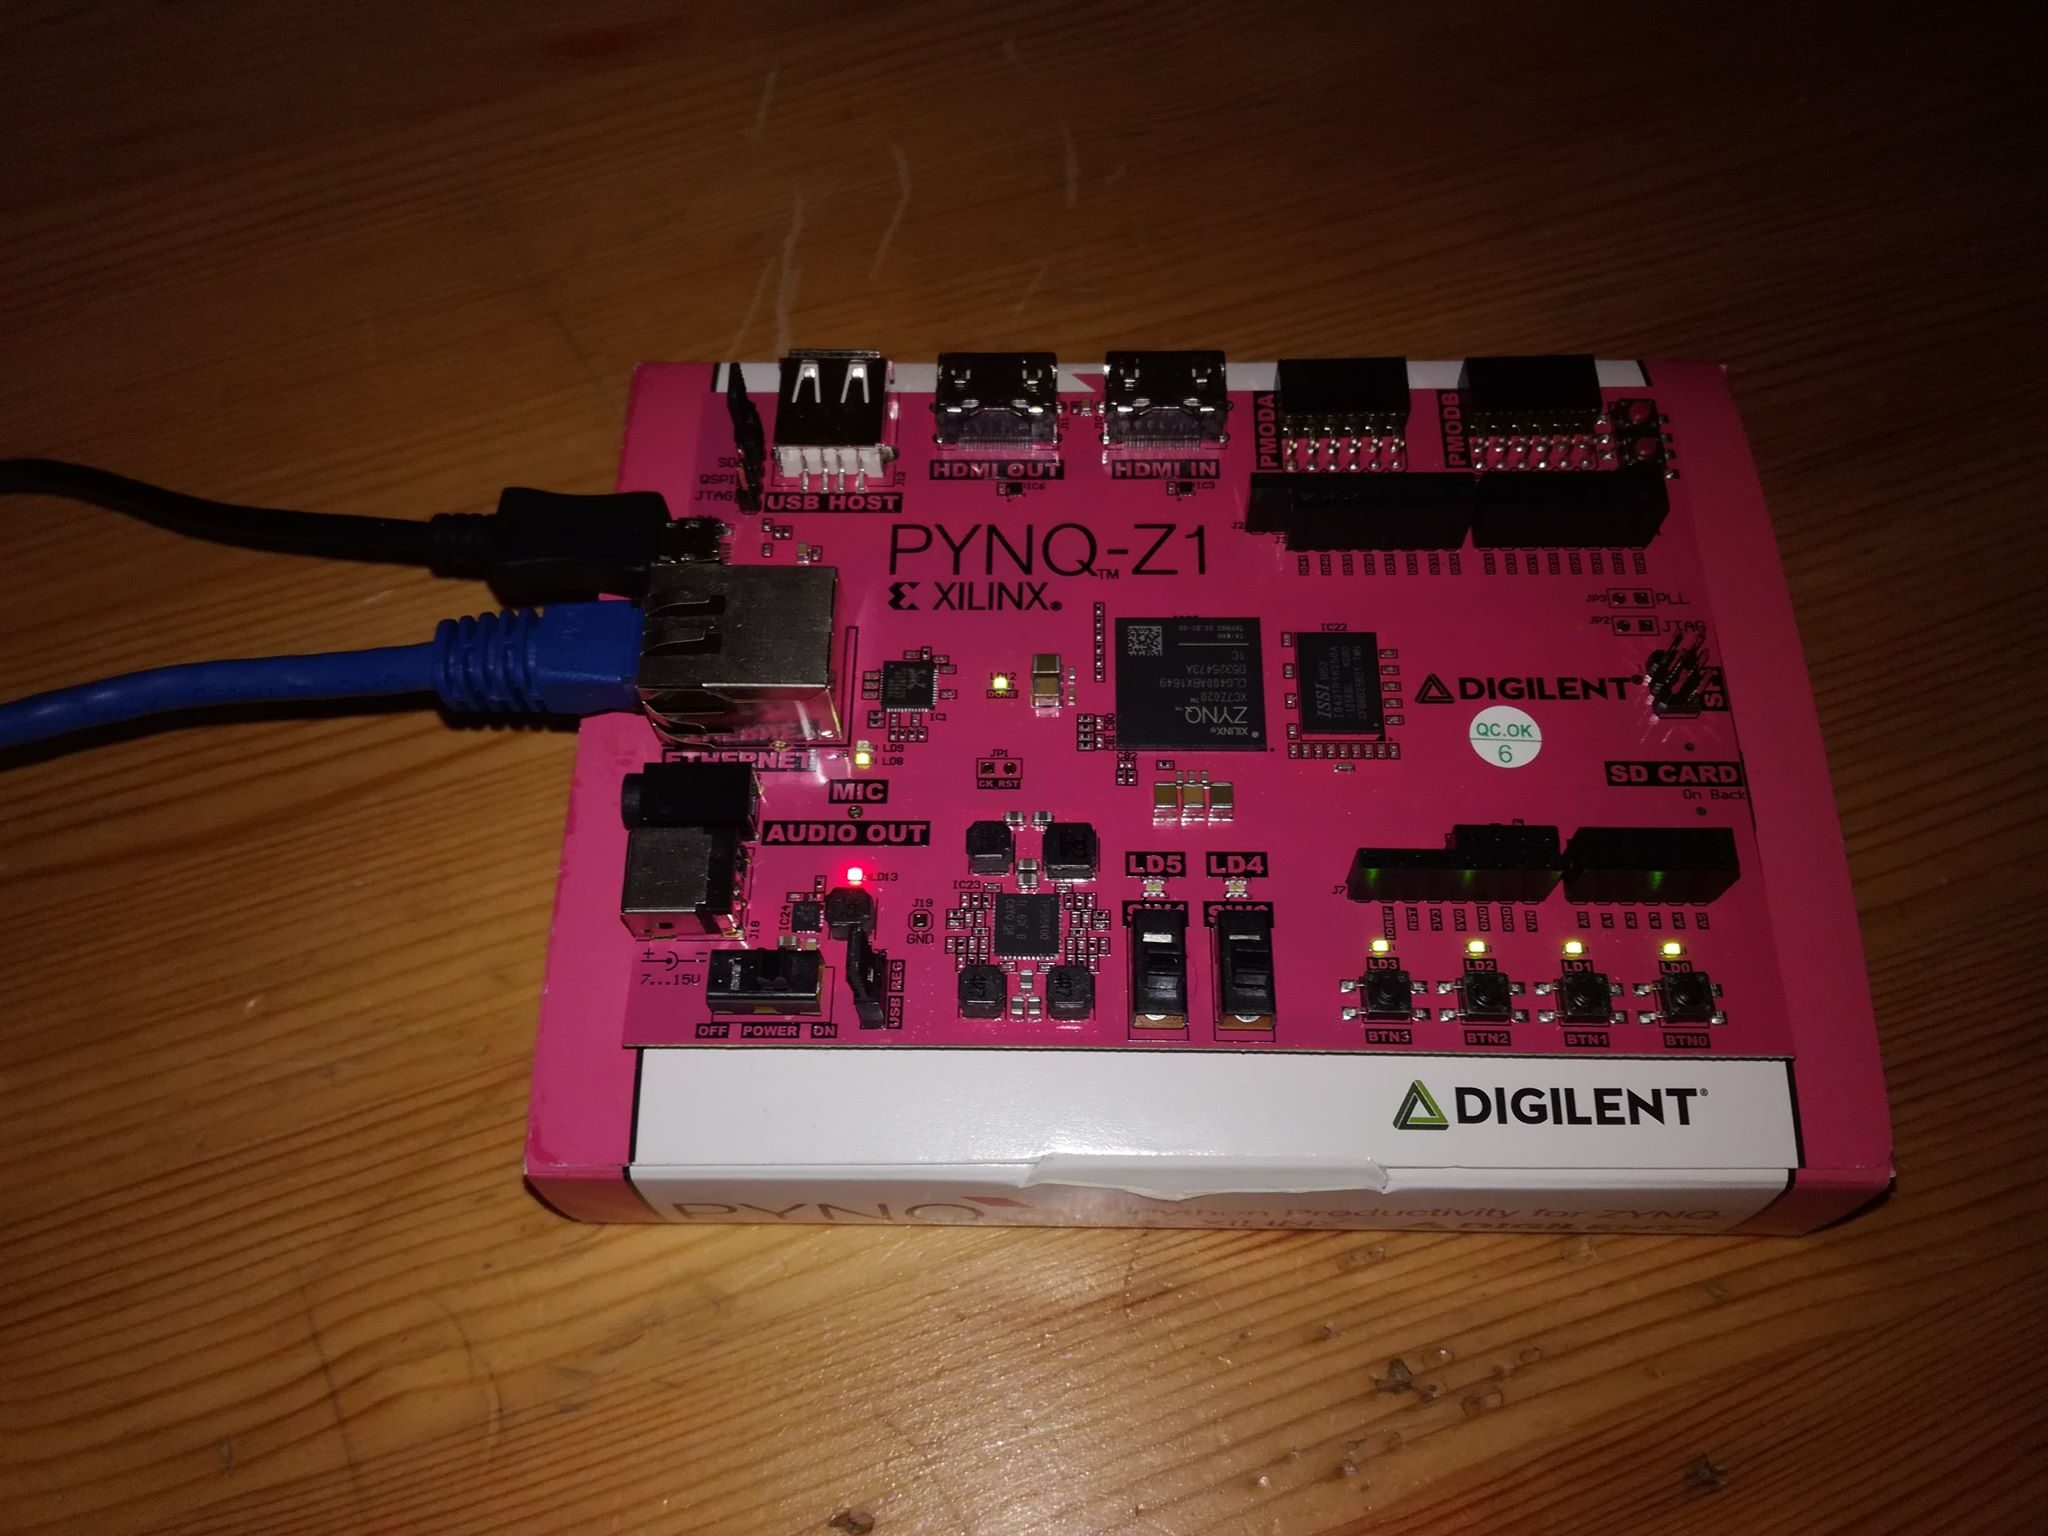
\includegraphics[width=12cm]{Figures/PYNQ.png}
	\caption[PYNQ-Z1]{PYNQ-Z1 with a neural network deployed}
	\label{fig:PYNQ-Z1}
\end{figure}


\newpage

In the end, it is possible to provide an image to the deployed network as presented on \emph{Listing} \ref{fig:DeployedInference}. This figure presents a script to first load the image and convert it to a tensor. Then, the trained transformed network is loaded and \texttt{onnx-exec} is used to run the image through the network. The result is then interpreted through the \texttt{softmax} function that outputs the different probabilities of each class for the provided picture.

\begin{mylisting}[htbp]
\centering
\begin{lstlisting}[language=Python]
import numpy as np
from \emph{FINN}.core.onnx_exec import execute_onnx
# Loading the image
image = Image.open('/workspace/finn/onnx_experiments/img_MNIST.png')
x = TF.to_tensor(image)
x.unsqueeze_(0)
# Loading the parent model of the partition
parent_model = load("dataflow_parent")
sdp_node = parent_model.graph.node[2]
remote_exec_model = build_dir + "tfc_deploy.onnx"
getCustomOp(sdp_node).set_nodeattr("model", remote_exec_model)
save(parent_model,"dataflow_parent_with_remote_bitfile_exec")
# Running the model, the deployed part will go to the FPGA once the node is reached
iname = parent_model.graph.input[0].name
oname = parent_model.graph.output[0].name
ishape = parent_model.get_tensor_shape(iname)
input_dict = {iname: x.numpy()[0].reshape(ishape)}
ret = execute_onnx(parent_model, input_dict, True)
# Definition of the softmax function
def softmax(x):
    """Compute softmax values for each sets of scores in x."""
    e_x = np.exp(x - np.max(x))
    return e_x / e_x.sum()
logits = ret[oname].flatten()
prob = softmax(logits)
# Presentation of the probabilities for the given image
plt.bar(np.arange(10), prob)
\end{lstlisting}
\caption[Deployed Inference]{Inference on the deployed network}
  \label{fig:DeployedInference}
\end{mylisting}

Moreover, \emph{FINN} provides a way to conduct a throughput test as presented on \emph{Listing} \ref{fig:ThroughputTest}. The test takes advantage of \emph{FINN} function \texttt{throughput\_test} that outputs both the throughput and other i/o metrics such as the DRAM bandwidth for example.

\begin{mylisting}[htbp]
\centering
\begin{lstlisting}[language=Python]
from \emph{FINN}.core.throughput_test import throughput_test

child_model = ModelWrapper(getCustomOp(sdp_node).get_nodeattr("model"))
res = throughput_test(child_model)
print("Network metrics:")
for key in res:
    print(str(key) + ": " + str(res[key]))
\end{lstlisting}
\caption[Throughput Test]{Throughput test method}
  \label{fig:ThroughputTest}
\end{mylisting}

\chapter{Results} % Main chapter title

\label{Chapter7} % For referencing this chapter elsewhere, use \ref{Chapter7}

\lhead{Chapter 7. \emph{Results}}

%----------------------------------------------------------------------------------------
%	SECTION 7.1 - Results Graphs
%----------------------------------------------------------------------------------------

\section{Results Graphs}

%----------------------------------------------------------------------------------------
%	SECTION 7.2 - Results Tables
%----------------------------------------------------------------------------------------

\section{Results Tables}

\chapter{Discussion \& Evaluation} % Main chapter title

\label{Chapter8} % For referencing this chapter elsewhere, use \ref{Chapter9}

\lhead{Chapter 8. \emph{Discussion \& Evaluation}}

%----------------------------------------------------------------------------------------
%	SECTION 8.1 - Discussion
%----------------------------------------------------------------------------------------

\section{Discussion}

%----------------------------------------------------------------------------------------
%	SECTION 8.2.1 - Network Architectures
%----------------------------------------------------------------------------------------

\subsection{Network Architectures}

The chosen architectures used during the experiments were supposed to be starting from \emph{LeNet-5} and go through well-known architectures such as \emph{AlexNet}, \emph{VGG-16} or \emph{Mobilenet}. However, while these implementations are able to train on a given dataset thanks to the developed benchmark, many of the implementations could not be exported to the intermediate representation. This is due to the fact that the export method and the delegates it uses are still in active development. Only simple layers successions have been implemented. This is why the only network that managed to run on the FPGA board is the \emph{TFC} (three successive fully-connected layers). This layer is known to have correct accuracy on the \emph{MNIST} dataset and uses only simple layers. The \emph{CNV} network corresponds to a simple CNN interconnected with \texttt{HardTanH} activations. This network has been trained as well but could not be deployed. The other networks are variations of the simple \emph{CNV} network and were not trained due to the amount of time and energy needed while obtaining only the first part of the workflow (through \emph{Brevitas}) in the end. The focus is put on hardware acceleration and this is why this choice was made.

While the training can be completed for any of the mentioned architectures, the scripts to deploy the other architectures will need to be extended. The extension should not be costly and would only be needed in the second part of the workflow: \emph{ONNX} and \emph{FINN}.

%----------------------------------------------------------------------------------------
%	SECTION 8.2.2 - Datasets
%----------------------------------------------------------------------------------------

\subsection{Datasets}

The architectures from earlier were supposed to go along with \emph{MNIST (or similar)} for the simpler networks, \emph{CIFAR-10} for the intermediate ones and either \emph{SVHN} or \emph{GTSRB} for the more complex architectures. The choice of those networks was made over \emph{ImageNet} due to the amount of time and energy training a network on \emph{ImageNet} would require. GTSRB seems like a correct compromise due to the number of classes it holds (over 40) and the emphasis around autonomous driving. In the end, the trainings were made on \emph{FashionMNIST}, a variation the \emph{MNIST} dataset as well as \emph{CIFAR-10} for the simple CNN. The \emph{GTSRB} dataset has been implemented in the benchmark to be used as it is not available by default in \emph{PyTorch} but any of the already provided datasets in \emph{PyTorch} can be easily added to the benchmark.


%----------------------------------------------------------------------------------------
%	SECTION 8.2.3 - Training Process
%----------------------------------------------------------------------------------------

\subsection{Training Process}

The training process was taken from \cite{Bethge2018} This process consists of a 40 epochs training with modifications to the learning rate (division by 10) at epochs 34 and 37. This training process uses the \emph{ADAM} optimiser such as recommended in \cite{Alizadeh2018}. The loss function by default is \emph{Cross Entropy} but the \emph{Square-Hinged} has been added as an extension to \emph{PyTorch} in order to be able to handle binarised neural networks. Any optimiser or loss function already defined by \emph{PyTorch} can be easily added to the benchmark.

%----------------------------------------------------------------------------------------
%	SECTION 8.2.4 - Deployment Process
%----------------------------------------------------------------------------------------

\subsection{Deployment Process}

The deployment process depends on two main points: \emph{Transformations} used and \emph{Folding} proposed. As presented earlier, the \emph{transformations} are very \guille{network specific} but several common ones can be extracted. Those transformations are still in active development and many of them will be simplified later on. Once the convolutions will be correctly handled, a higher-level API can be used. On the other hand, the \emph{folding} is extremely \guille{network specific} as well and will also depends on the board used. For now, a folding factor can be chosen arbitrarily and specified by hand in the folding transformations. This is supposed to be handled automatically depending on the hardware resources available and provided. This should be available in later versions of \emph{FINN}. In the presented experiments, the chosen folding factors was 32 and this means the FPGA will have to run 32 passes to process one image. This uses a little over 50\% of the available hardware resources on the FPGA. A divisibility argument has to be kept and using a folding factor of 16 would require over 110\% of the board resources and would therefore not be able to complete the deployment. This parameter can and should be tuned more finely in the future.

%----------------------------------------------------------------------------------------
%	SECTION 8.2.5 - Weight and Activation Bitwidths
%----------------------------------------------------------------------------------------

\subsection{Weight and Activation Bitwidths}

The activation bitwidth used were taken specifically to be comparable. This means that the binarised network would require both slightly different forward functions and another loss function. This is why only activations and weights from 2 to 32 bits (2, 4, 8, 16 and 32) were chosen and used. Contrary to \cite{Bacchus2020}, no difference has been made between the activations and weights bitwidths. This is due to the fact that for now, \emph{FINN} cannot handle quantised neural networks with higher bitwidth for activations than weights. Once the feature is made available, the integration to the benchmark is instantaneous as it should already be possible. In addition to the weights and activations bitwidth, an input bitwidth has been provided to be used on the first layer of the network architecture. This is done to prevent harsh quantisation from degrading the end accuracy too much.

%----------------------------------------------------------------------------------------
%	SECTION 8.3 - Evaluation
%----------------------------------------------------------------------------------------

\section{Evaluation}

%----------------------------------------------------------------------------------------
%	SUBSECTION 8.3.1 - Comparison to the literature
%----------------------------------------------------------------------------------------

\subsection{Comparison to the literature}

% TODO COMPARISON LITERATURE

Comparison \emph{TFC} / \emph{Fashion-MNIST} with other results from the literature.

Comparison \emph{CNV} / \emph{CIFAR-10} with other results from the literature.
%----------------------------------------------------------------------------------------
%	SUBSECTION 8.3.2 - Future Works
%----------------------------------------------------------------------------------------

\subsection{Future Works}

The discussion section presented several points that will need to be extended in the future. First of all, using well-known network architectures is extremely important as they have been thoroughly studied and benchmarked. The same goes for the datasets and requires no effort from the \emph{Brevitas} development team as it is already available in PyTorch. While any network can be trained on any dataset for now, the issue comes from the latter parts of the workflow. The export does not cover all the layer configurations for now and other benchmarks will need to be conducted to cover the new architectures and their coupled datasets. \emph{FINN} is not available to handle every architecture for now but several well-known architectures are planned to be supported. For example, \emph{Mobilenet} should run through the whole cycle by the beginning of September this year. Once the end-to-end flow is working, additional benchmarking will be available at a small development cost. As presented in \cite{Bacchus2020}, the difference between the bitwidth of activations and weights will have to be differentiated in order to be evaluated separately and allow to write guidelines.

Overall, the development of the benchmark highlighted a surprising result that will need explanations from the Xilinx development team because it goes against all the objectives and the underlying idea of reduced precision. This result also shows the importance of benchmarks to assess the different ideas one might have when coming into hardware acceleration. \emph{FINN} is, for now, actively developed and open-source, gathering a growing community. However, the same type of benchmarking could be performed on other FPGA frameworks such as the ones presented in \ref{Chapter3}, \cite{Andri2016, Zhao2016, Venieris2017, Ding2019, Jahanshahi2019}. However, those frameworks have their code source closed and would require a lot more time and effort to investigate and benchmark. On the other hand, comparison with classic quantisation and compression frameworks (i.e. that do not require to be deployed on an FPGA board) would be interesting. Working with Intel\'s \emph{Distiller} \cite{Nzmora2019} for example or the newly added quantisation packages in \emph{PyTorch} or \emph{TensorFlow}.

\chapter{Conclusion} % Main chapter title

\label{Chapter9} % For referencing this chapter elsewhere, use \ref{Chapter9}

\lhead{Chapter 9. \emph{Future Works \& Conclusion}}

The objectives of this document are to present the many interests behind reduced- and mixed- precision in modern applications. Literature has been put under examination to determine the interests of mixed-precision, the methods that can be used to put it in action and the applications it can have on state-to-the-art projects and research fields. The most important take on mixed-precision is to get rid of superfluous precision, often set by default by the developer early in the development process, to gain performance while losing a negligible amount of precision. Several methods such as iterative refinement or automated tuning can be used to apply mixed-precision to real-world applications in scientific computations.

The literature review highlights several applications but one has been chosen to be further developed. The case of deep learning applied to reconfigurable architectures can highlight the use of mixed-precision along with a novel piece of hardware that fits the application. The implementation of the process will present important parameters contained in the neural network and present the impact of their size and precision on the overall performance and associated precision. FPGAs are a good fit for this application as each of the parameters can be linked to a tailored space and area in the hardware design.

The next step after this research report is the development of the project itself and the redaction of the dissertation presenting the reasoning behind the decisions taken during the development as well as the results obtained and their implications. Results can and should lead to guidelines as well as recommendations for future works and protections put into place.


%----------------------------------------------------------------------------------------
%	THESIS CONTENT - APPENDICES
%----------------------------------------------------------------------------------------

\addtocontents{toc}{\vspace{2em}} % Add a gap in the Contents, for aesthetics

\appendix % Cue to tell LaTeX that the following 'chapters' are Appendices

% Include the appendices of the thesis as separate files from the Appendices folder
% Uncomment the lines as you write the Appendices

% Appendix A

\chapter{Hardware Utilisation Results} % Main appendix title

\label{AppendixA} % For referencing this appendix elsewhere, use \ref{AppendixA}

\lhead{Appendix A. \emph{Hardware Utilisation Results}} % This is for the header on each page - perhaps a shortened title

This appendix contains the detailed results of the hardware utilisation for the different configuration. In the tables can be found the total number of resources used under the \texttt{resizer\_wrapper}, the used resources for the important \emph{IP}s of the system following and the different layers that begin with \texttt{Streaming...}.



\begin{landscape}

\begin{table}[!htb]
\resizebox{24cm}{!}{
\begin{tabular}{l|l|l|l|l|l|l|l|l|l|l}
   \textbf{Instance}                                         & \textbf{Module}                                                                                        & \textbf{Total LUTs} & \textbf{Logic LUTs} & \textbf{LUTRAMs} & \textbf{SRLs} & \textbf{FFs}   & \textbf{RAMB36} & \textbf{RAMB18} & \textbf{DSP48 Blocks} \\
   resizer\_wrapper                                        & (top)                                                                                                  & 31622      & 28324      & 1302    & 1996 & 27989 & 40     & 3      & 0            \\
   resizer\_i                                              & resizer                                                                                                & 31622      & 28324      & 1302    & 1996 & 27989 & 40     & 3      & 0            \\
   axi\_dma\_0                                             & resizer\_axi\_dma\_0\_0                                                                                & 1960       & 1750       & 12      & 198  & 2626  & 8      & 2      & 0            \\
   axi\_interconnect\_0                                    & resizer\_axi\_interconnect\_0\_0                                                                       & 551        & 486        & 0       & 65   & 694   & 0      & 0      & 0            \\
   axi\_protocol\_convert\_0                               & resizer\_axi\_protocol\_convert\_0\_0                                                                  & 393        & 383        & 10      & 0    & 430   & 0      & 0      & 0            \\
   axis\_dwidth\_converter\_0                              & resizer\_axis\_dwidth\_converter\_0\_0                                                                 & 21         & 21         & 0       & 0    & 370   & 0      & 0      & 0            \\
   axis\_dwidth\_converter\_1                              & resizer\_axis\_dwidth\_converter\_1\_0                                                                 & 335        & 335        & 0       & 0    & 995   & 0      & 0      & 0            \\
   processing\_system7\_0                                  & resizer\_processing\_system7\_0\_0                                                                     & 112        & 112        & 0       & 0    & 0     & 0      & 0      & 0            \\
   resize\_accel\_0                                        & resizer\_resize\_accel\_0\_0                                                                           & 28231      & 25219      & 1280    & 1732 & 22834 & 32     & 1      & 0            \\
   rst\_ps7\_0\_100M                                       & resizer\_rst\_ps7\_0\_100M\_0                                                                          & 19         & 18         & 0       & 1    & 40    & 0      & 0      & 0            \\
   StreamingDataWidthConverter\_Batch\_0                   & resizer\_resize\_accel\_0\_0\_finn\_design\_StreamingDataWidthConverter\_Batch\_0\_0                   & 101        & 101        & 0       & 0    & 196   & 0      & 0      & 0            \\
   StreamingFCLayer\_Batch\_0                              & resizer\_resize\_accel\_0\_0\_finn\_design\_StreamingFCLayer\_Batch\_0\_0                              & 19464      & 18439      & 0       & 1025 & 16314 & 28     & 1      & 0            \\
   StreamingFCLayer\_Batch\_1                              & resizer\_resize\_accel\_0\_0\_finn\_design\_StreamingFCLayer\_Batch\_1\_0                              & 2254       & 2189       & 0       & 65   & 1634  & 2      & 0      & 0            \\
   StreamingFCLayer\_Batch\_2                              & resizer\_resize\_accel\_0\_0\_finn\_design\_StreamingFCLayer\_Batch\_2\_0                              & 2260       & 2195       & 0       & 65   & 1640  & 2      & 0      & 0            \\
   StreamingFCLayer\_Batch\_3                              & resizer\_resize\_accel\_0\_0\_finn\_design\_StreamingFCLayer\_Batch\_3\_0                              & 2472       & 1111       & 1280    & 81   & 1491  & 0      & 0      & 0            \\
   StreamingFIFO\_0                                        & resizer\_resize\_accel\_0\_0\_finn\_design\_StreamingFIFO\_0\_0                                        & 542        & 286        & 0       & 256  & 276   & 0      & 0      & 0            \\
   StreamingFIFO\_1                                        & resizer\_resize\_accel\_0\_0\_finn\_design\_StreamingFIFO\_1\_0                                        & 91         & 59         & 0       & 32   & 42    & 0      & 0      & 0            \\
   StreamingFIFO\_2                                        & resizer\_resize\_accel\_0\_0\_finn\_design\_StreamingFIFO\_2\_0                                        & 59         & 43         & 0       & 16   & 26    & 0      & 0      & 0            \\
   StreamingFIFO\_3                                        & resizer\_resize\_accel\_0\_0\_finn\_design\_StreamingFIFO\_3\_0                                        & 59         & 43         & 0       & 16   & 26    & 0      & 0      & 0            \\
   StreamingFIFO\_4                                        & resizer\_resize\_accel\_0\_0\_finn\_design\_StreamingFIFO\_4\_0                                        & 59         & 43         & 0       & 16   & 26    & 0      & 0      & 0            \\
   StreamingFIFO\_5                                        & resizer\_resize\_accel\_0\_0\_finn\_design\_StreamingFIFO\_5\_0                                        & 338        & 178        & 0       & 160  & 169   & 0      & 0      & 0            \\
   TLastMarker\_0                                          & resizer\_resize\_accel\_0\_0\_finn\_design\_TLastMarker\_0\_0                                          & 532        & 532        & 0       & 0    & 994   & 0      & 0      & 0            \\
\end{tabular}
}
\caption[TFC Hardware Utilisation A2W2]{TFC Hardware Utilisation for A2W2 configuration}
  \label{tab:TFCHardwareA2W2}
\end{table}


\begin{table}[!htb]
\resizebox{24cm}{!}{
\begin{tabular}{l|l|l|l|l|l|l|l|l|l|l}
   \textbf{Instance}                                         & \textbf{Module}                                                                                        & \textbf{Total LUTs} & \textbf{Logic LUTs} & \textbf{LUTRAMs} & \textbf{SRLs} & \textbf{FFs}   & \textbf{RAMB36} & \textbf{RAMB18} & \textbf{DSP48 Blocks} \\
   resizer\_wrapper                                        & (top)                                                                                                  & 31614      & 28316      & 1302    & 1996 & 28052 & 40     & 3      & 0            \\
   resizer\_i                                              & resizer                                                                                                & 31614      & 28316      & 1302    & 1996 & 28052 & 40     & 3      & 0            \\
   axi\_dma\_0                                             & resizer\_axi\_dma\_0\_0                                                                                & 1960       & 1750       & 12      & 198  & 2626  & 8      & 2      & 0            \\
   axi\_interconnect\_0                                    & resizer\_axi\_interconnect\_0\_0                                                                       & 551        & 486        & 0       & 65   & 694   & 0      & 0      & 0            \\
   axi\_protocol\_convert\_0                               & resizer\_axi\_protocol\_convert\_0\_0                                                                  & 393        & 383        & 10      & 0    & 430   & 0      & 0      & 0            \\
   axis\_dwidth\_converter\_0                              & resizer\_axis\_dwidth\_converter\_0\_0                                                                 & 21         & 21         & 0       & 0    & 370   & 0      & 0      & 0            \\
   axis\_dwidth\_converter\_1                              & resizer\_axis\_dwidth\_converter\_1\_0                                                                 & 335        & 335        & 0       & 0    & 995   & 0      & 0      & 0            \\
   processing\_system7\_0                                  & resizer\_processing\_system7\_0\_0                                                                     & 112        & 112        & 0       & 0    & 0     & 0      & 0      & 0            \\
   resize\_accel\_0                                        & resizer\_resize\_accel\_0\_0                                                                           & 28223      & 25211      & 1280    & 1732 & 22897 & 32     & 1      & 0            \\
   rst\_ps7\_0\_100M                                       & resizer\_rst\_ps7\_0\_100M\_0                                                                          & 19         & 18         & 0       & 1    & 40    & 0      & 0      & 0            \\
   StreamingDataWidthConverter\_Batch\_0                   & resizer\_resize\_accel\_0\_0\_finn\_design\_StreamingDataWidthConverter\_Batch\_0\_0                   & 101        & 101        & 0       & 0    & 196   & 0      & 0      & 0            \\
   StreamingFCLayer\_Batch\_0                              & resizer\_resize\_accel\_0\_0\_finn\_design\_StreamingFCLayer\_Batch\_0\_0                              & 19505      & 18480      & 0       & 1025 & 16461 & 28     & 1      & 0            \\
   StreamingFCLayer\_Batch\_1                              & resizer\_resize\_accel\_0\_0\_finn\_design\_StreamingFCLayer\_Batch\_1\_0                              & 2223       & 2158       & 0       & 65   & 1583  & 2      & 0      & 0            \\
   StreamingFCLayer\_Batch\_2                              & resizer\_resize\_accel\_0\_0\_finn\_design\_StreamingFCLayer\_Batch\_2\_0                              & 2242       & 2177       & 0       & 65   & 1607  & 2      & 0      & 0            \\
   StreamingFCLayer\_Batch\_3                              & resizer\_resize\_accel\_0\_0\_finn\_design\_StreamingFCLayer\_Batch\_3\_0                              & 2472       & 1111       & 1280    & 81   & 1491  & 0      & 0      & 0            \\
   StreamingFIFO\_0                                        & resizer\_resize\_accel\_0\_0\_finn\_design\_StreamingFIFO\_0\_0                                        & 542        & 286        & 0       & 256  & 276   & 0      & 0      & 0            \\
   StreamingFIFO\_1                                        & resizer\_resize\_accel\_0\_0\_finn\_design\_StreamingFIFO\_1\_0                                        & 91         & 59         & 0       & 32   & 42    & 0      & 0      & 0            \\
   StreamingFIFO\_2                                        & resizer\_resize\_accel\_0\_0\_finn\_design\_StreamingFIFO\_2\_0                                        & 59         & 43         & 0       & 16   & 26    & 0      & 0      & 0            \\
   StreamingFIFO\_3                                        & resizer\_resize\_accel\_0\_0\_finn\_design\_StreamingFIFO\_3\_0                                        & 59         & 43         & 0       & 16   & 26    & 0      & 0      & 0            \\
   StreamingFIFO\_4                                        & resizer\_resize\_accel\_0\_0\_finn\_design\_StreamingFIFO\_4\_0                                        & 59         & 43         & 0       & 16   & 26    & 0      & 0      & 0            \\
   StreamingFIFO\_5                                        & resizer\_resize\_accel\_0\_0\_finn\_design\_StreamingFIFO\_5\_0                                        & 338        & 178        & 0       & 160  & 169   & 0      & 0      & 0            \\
   TLastMarker\_0                                          & resizer\_resize\_accel\_0\_0\_finn\_design\_TLastMarker\_0\_0                                          & 532        & 532        & 0       & 0    & 994   & 0      & 0      & 0            \\
\end{tabular}
}
\caption[TFC Hardware Utilisation A4W4]{TFC Hardware Utilisation for A4W4 configuration}
  \label{tab:TFCHardwareA4W4}
\end{table}

\begin{table}[!htb]
\resizebox{24cm}{!}{
\begin{tabular}{l|l|l|l|l|l|l|l|l|l|l}
   \textbf{Instance}                                         & \textbf{Module}                                                                                        & \textbf{Total LUTs} & \textbf{Logic LUTs} & \textbf{LUTRAMs} & \textbf{SRLs} & \textbf{FFs}   & \textbf{RAMB36} & \textbf{RAMB18} & \textbf{DSP48 Blocks} \\
   resizer\_wrapper                                        & (top)                                                                                                & 31653      & 28355      & 1302    & 1996 & 27953 & 40     & 3      & 0            \\
   resizer\_i                                              & resizer                                                                                              & 31653      & 28355      & 1302    & 1996 & 27953 & 40     & 3      & 0            \\
   axi\_dma\_0                                             & resizer\_axi\_dma\_0\_0                                                                              & 1960       & 1750       & 12      & 198  & 2626  & 8      & 2      & 0            \\
   axi\_interconnect\_0                                    & resizer\_axi\_interconnect\_0\_0                                                                     & 551        & 486        & 0       & 65   & 694   & 0      & 0      & 0            \\
   axi\_protocol\_convert\_0                               & resizer\_axi\_protocol\_convert\_0\_0                                                                & 393        & 383        & 10      & 0    & 430   & 0      & 0      & 0            \\
   axis\_dwidth\_converter\_0                              & resizer\_axis\_dwidth\_converter\_0\_0                                                               & 21         & 21         & 0       & 0    & 370   & 0      & 0      & 0            \\
   axis\_dwidth\_converter\_1                              & resizer\_axis\_dwidth\_converter\_1\_0                                                               & 335        & 335        & 0       & 0    & 995   & 0      & 0      & 0            \\
   processing\_system7\_0                                  & resizer\_processing\_system7\_0\_0                                                                   & 112        & 112        & 0       & 0    & 0     & 0      & 0      & 0            \\
   resize\_accel\_0                                        & resizer\_resize\_accel\_0\_0                                                                         & 28262      & 25250      & 1280    & 1732 & 22798 & 32     & 1      & 0            \\
   rst\_ps7\_0\_100M                                       & resizer\_rst\_ps7\_0\_100M\_0                                                                        & 19         & 18         & 0       & 1    & 40    & 0      & 0      & 0            \\
   StreamingDataWidthConverter\_Batch\_0                   & resizer\_resize\_accel\_0\_0\_finn\_design\_StreamingDataWidthConverter\_Batch\_0\_0                 & 101        & 101        & 0       & 0    & 196   & 0      & 0      & 0            \\
   StreamingFCLayer\_Batch\_0                              & resizer\_resize\_accel\_0\_0\_finn\_design\_StreamingFCLayer\_Batch\_0\_0                            & 19568      & 18543      & 0       & 1025 & 16406 & 28     & 1      & 0            \\
   StreamingFCLayer\_Batch\_1                              & resizer\_resize\_accel\_0\_0\_finn\_design\_StreamingFCLayer\_Batch\_1\_0                            & 2217       & 2152       & 0       & 65   & 1557  & 2      & 0      & 0            \\
   StreamingFCLayer\_Batch\_2                              & resizer\_resize\_accel\_0\_0\_finn\_design\_StreamingFCLayer\_Batch\_2\_0                            & 2224       & 2159       & 0       & 65   & 1589  & 2      & 0      & 0            \\
   StreamingFCLayer\_Batch\_3                              & resizer\_resize\_accel\_0\_0\_finn\_design\_StreamingFCLayer\_Batch\_3\_0                            & 2472       & 1111       & 1280    & 81   & 1491  & 0      & 0      & 0            \\
   StreamingFIFO\_0                                        & resizer\_resize\_accel\_0\_0\_finn\_design\_StreamingFIFO\_0\_0                                      & 542        & 286        & 0       & 256  & 276   & 0      & 0      & 0            \\
   StreamingFIFO\_1                                        & resizer\_resize\_accel\_0\_0\_finn\_design\_StreamingFIFO\_1\_0                                      & 91         & 59         & 0       & 32   & 42    & 0      & 0      & 0            \\
   StreamingFIFO\_2                                        & resizer\_resize\_accel\_0\_0\_finn\_design\_StreamingFIFO\_2\_0                                      & 59         & 43         & 0       & 16   & 26    & 0      & 0      & 0            \\
   StreamingFIFO\_3                                        & resizer\_resize\_accel\_0\_0\_finn\_design\_StreamingFIFO\_3\_0                                      & 59         & 43         & 0       & 16   & 26    & 0      & 0      & 0            \\
   StreamingFIFO\_4                                        & resizer\_resize\_accel\_0\_0\_finn\_design\_StreamingFIFO\_4\_0                                      & 59         & 43         & 0       & 16   & 26    & 0      & 0      & 0            \\
   StreamingFIFO\_5                                        & resizer\_resize\_accel\_0\_0\_finn\_design\_StreamingFIFO\_5\_0                                      & 338        & 178        & 0       & 160  & 169   & 0      & 0      & 0            \\
   TLastMarker\_0                                          & resizer\_resize\_accel\_0\_0\_finn\_design\_TLastMarker\_0\_0                                        & 532        & 532        & 0       & 0    & 994   & 0      & 0      & 0            \\
\end{tabular}
}
\caption[TFC Hardware Utilisation A8W8]{TFC Hardware Utilisation for A8W8 configuration}
  \label{tab:TFCHardwareA8W8}
\end{table}

\begin{table}[!htb]
\resizebox{24cm}{!}{
\begin{tabular}{l|l|l|l|l|l|l|l|l|l|l}
   \textbf{Instance}                                         & \textbf{Module}                                                                                        & \textbf{Total LUTs} & \textbf{Logic LUTs} & \textbf{LUTRAMs} & \textbf{SRLs} & \textbf{FFs}   & \textbf{RAMB36} & \textbf{RAMB18} & \textbf{DSP48 Blocks} \\
   resizer\_wrapper                                        & (top)                                                                                                  & 31612      & 28314      & 1302    & 1996 & 27997 & 40     & 3      & 0            \\
   resizer\_i                                              & resizer                                                                                                & 31612      & 28314      & 1302    & 1996 & 27997 & 40     & 3      & 0            \\
   axi\_dma\_0                                             & resizer\_axi\_dma\_0\_0                                                                                & 1960       & 1750       & 12      & 198  & 2626  & 8      & 2      & 0            \\
   axi\_interconnect\_0                                    & resizer\_axi\_interconnect\_0\_0                                                                       & 551        & 486        & 0       & 65   & 694   & 0      & 0      & 0            \\
   axi\_protocol\_convert\_0                               & resizer\_axi\_protocol\_convert\_0\_0                                                                  & 393        & 383        & 10      & 0    & 430   & 0      & 0      & 0            \\
   axis\_dwidth\_converter\_0                              & resizer\_axis\_dwidth\_converter\_0\_0                                                                 & 21         & 21         & 0       & 0    & 370   & 0      & 0      & 0            \\
   axis\_dwidth\_converter\_1                              & resizer\_axis\_dwidth\_converter\_1\_0                                                                 & 335        & 335        & 0       & 0    & 995   & 0      & 0      & 0            \\
   processing\_system7\_0                                  & resizer\_processing\_system7\_0\_0                                                                     & 112        & 112        & 0       & 0    & 0     & 0      & 0      & 0            \\
   resize\_accel\_0                                        & resizer\_resize\_accel\_0\_0                                                                           & 28221      & 25209      & 1280    & 1732 & 22842 & 32     & 1      & 0            \\
   rst\_ps7\_0\_100M                                       & resizer\_rst\_ps7\_0\_100M\_0                                                                          & 19         & 18         & 0       & 1    & 40    & 0      & 0      & 0            \\
   StreamingDataWidthConverter\_Batch\_0                   & resizer\_resize\_accel\_0\_0\_finn\_design\_StreamingDataWidthConverter\_Batch\_0\_0                   & 101        & 101        & 0       & 0    & 196   & 0      & 0      & 0            \\
   StreamingFCLayer\_Batch\_0                              & resizer\_resize\_accel\_0\_0\_finn\_design\_StreamingFCLayer\_Batch\_0\_0                              & 19521      & 18496      & 0       & 1025 & 16462 & 28     & 1      & 0            \\
   StreamingFCLayer\_Batch\_1                              & resizer\_resize\_accel\_0\_0\_finn\_design\_StreamingFCLayer\_Batch\_1\_0                              & 2218       & 2153       & 0       & 65   & 1559  & 2      & 0      & 0            \\
   StreamingFCLayer\_Batch\_2                              & resizer\_resize\_accel\_0\_0\_finn\_design\_StreamingFCLayer\_Batch\_2\_0                              & 2229       & 2164       & 0       & 65   & 1575  & 2      & 0      & 0            \\
   StreamingFCLayer\_Batch\_3                              & resizer\_resize\_accel\_0\_0\_finn\_design\_StreamingFCLayer\_Batch\_3\_0                              & 2472       & 1111       & 1280    & 81   & 1491  & 0      & 0      & 0            \\
   StreamingFIFO\_0                                        & resizer\_resize\_accel\_0\_0\_finn\_design\_StreamingFIFO\_0\_0                                        & 542        & 286        & 0       & 256  & 276   & 0      & 0      & 0            \\
   StreamingFIFO\_1                                        & resizer\_resize\_accel\_0\_0\_finn\_design\_StreamingFIFO\_1\_0                                        & 91         & 59         & 0       & 32   & 42    & 0      & 0      & 0            \\
   StreamingFIFO\_2                                        & resizer\_resize\_accel\_0\_0\_finn\_design\_StreamingFIFO\_2\_0                                        & 59         & 43         & 0       & 16   & 26    & 0      & 0      & 0            \\
   StreamingFIFO\_3                                        & resizer\_resize\_accel\_0\_0\_finn\_design\_StreamingFIFO\_3\_0                                        & 59         & 43         & 0       & 16   & 26    & 0      & 0      & 0            \\
   StreamingFIFO\_4                                        & resizer\_resize\_accel\_0\_0\_finn\_design\_StreamingFIFO\_4\_0                                        & 59         & 43         & 0       & 16   & 26    & 0      & 0      & 0            \\
   TLastMarker\_0                                          & resizer\_resize\_accel\_0\_0\_finn\_design\_TLastMarker\_0\_0                                          & 532        & 532        & 0       & 0    & 994   & 0      & 0      & 0            \\
\end{tabular}
}
\caption[TFC Hardware Utilisation A16W16]{TFC Hardware Utilisation for A16W16 configuration}
  \label{tab:TFCHardwareA16W16}
\end{table}


\begin{table}[!htb]
\resizebox{24cm}{!}{
\begin{tabular}{l|l|l|l|l|l|l|l|l|l|l}
   \textbf{Instance}                                         & \textbf{Module}                                                                                        & \textbf{Total LUTs} & \textbf{Logic LUTs} & \textbf{LUTRAMs} & \textbf{SRLs} & \textbf{FFs}   & \textbf{RAMB36} & \textbf{RAMB18} & \textbf{DSP48 Blocks} \\
   resizer\_wrapper                                        & (top)                                                                                                  & 31599      & 28301      & 1302    & 1996 & 27949 & 40     & 3      & 0            \\
   resizer\_i                                              & resizer                                                                                                & 31599      & 28301      & 1302    & 1996 & 27949 & 40     & 3      & 0            \\
   axi\_dma\_0                                             & resizer\_axi\_dma\_0\_0                                                                                & 1960       & 1750       & 12      & 198  & 2626  & 8      & 2      & 0            \\
   axi\_interconnect\_0                                    & resizer\_axi\_interconnect\_0\_0                                                                       & 551        & 486        & 0       & 65   & 694   & 0      & 0      & 0            \\
   axi\_protocol\_convert\_0                               & resizer\_axi\_protocol\_convert\_0\_0                                                                  & 393        & 383        & 10      & 0    & 430   & 0      & 0      & 0            \\
   axis\_dwidth\_converter\_0                              & resizer\_axis\_dwidth\_converter\_0\_0                                                                 & 21         & 21         & 0       & 0    & 370   & 0      & 0      & 0            \\
   axis\_dwidth\_converter\_1                              & resizer\_axis\_dwidth\_converter\_1\_0                                                                 & 335        & 335        & 0       & 0    & 995   & 0      & 0      & 0            \\
   processing\_system7\_0                                  & resizer\_processing\_system7\_0\_0                                                                     & 112        & 112        & 0       & 0    & 0     & 0      & 0      & 0            \\
   resize\_accel\_0                                        & resizer\_resize\_accel\_0\_0                                                                           & 28208      & 25196      & 1280    & 1732 & 22794 & 32     & 1      & 0            \\
   rst\_ps7\_0\_100M                                       & resizer\_rst\_ps7\_0\_100M\_0                                                                          & 19         & 18         & 0       & 1    & 40    & 0      & 0      & 0            \\
   StreamingDataWidthConverter\_Batch\_0                   & resizer\_resize\_accel\_0\_0\_finn\_design\_StreamingDataWidthConverter\_Batch\_0\_0                   & 101        & 101        & 0       & 0    & 196   & 0      & 0      & 0            \\
   StreamingFCLayer\_Batch\_0                              & resizer\_resize\_accel\_0\_0\_finn\_design\_StreamingFCLayer\_Batch\_0\_0                              & 19511      & 18486      & 0       & 1025 & 16414 & 28     & 1      & 0            \\
   StreamingFCLayer\_Batch\_1                              & resizer\_resize\_accel\_0\_0\_finn\_design\_StreamingFCLayer\_Batch\_1\_0                              & 2217       & 2152       & 0       & 65   & 1554  & 2      & 0      & 0            \\
   StreamingFCLayer\_Batch\_2                              & resizer\_resize\_accel\_0\_0\_finn\_design\_StreamingFCLayer\_Batch\_2\_0                              & 2227       & 2162       & 0       & 65   & 1580  & 2      & 0      & 0            \\
   StreamingFCLayer\_Batch\_3                              & resizer\_resize\_accel\_0\_0\_finn\_design\_StreamingFCLayer\_Batch\_3\_0                              & 2472       & 1111       & 1280    & 81   & 1491  & 0      & 0      & 0            \\
   StreamingFIFO\_0                                        & resizer\_resize\_accel\_0\_0\_finn\_design\_StreamingFIFO\_0\_0                                        & 542        & 286        & 0       & 256  & 276   & 0      & 0      & 0            \\
   StreamingFIFO\_1                                        & resizer\_resize\_accel\_0\_0\_finn\_design\_StreamingFIFO\_1\_0                                        & 91         & 59         & 0       & 32   & 42    & 0      & 0      & 0            \\
   StreamingFIFO\_2                                        & resizer\_resize\_accel\_0\_0\_finn\_design\_StreamingFIFO\_2\_0                                        & 59         & 43         & 0       & 16   & 26    & 0      & 0      & 0            \\
   StreamingFIFO\_3                                        & resizer\_resize\_accel\_0\_0\_finn\_design\_StreamingFIFO\_3\_0                                        & 59         & 43         & 0       & 16   & 26    & 0      & 0      & 0            \\
   StreamingFIFO\_4                                        & resizer\_resize\_accel\_0\_0\_finn\_design\_StreamingFIFO\_4\_0                                        & 59         & 43         & 0       & 16   & 26    & 0      & 0      & 0            \\
   StreamingFIFO\_5                                        & resizer\_resize\_accel\_0\_0\_finn\_design\_StreamingFIFO\_5\_0                                        & 338        & 178        & 0       & 160  & 169   & 0      & 0      & 0            \\
   TLastMarker\_0                                          & resizer\_resize\_accel\_0\_0\_finn\_design\_TLastMarker\_0\_0                                          & 532        & 532        & 0       & 0    & 994   & 0      & 0      & 0            \\
\end{tabular}
}
\caption[TFC Hardware Utilisation A32W32]{TFC Hardware Utilisation for A32W32 configuration}
  \label{tab:TFCHardwareA32W32}
\end{table}

\end{landscape}

%\input{Appendices/AppendixB}
%\input{Appendices/AppendixC}

\addtocontents{toc}{\vspace{2em}} % Add a gap in the Contents, for aesthetics

\backmatter

%----------------------------------------------------------------------------------------
%	BIBLIOGRAPHY
%----------------------------------------------------------------------------------------

\label{Bibliography}

\lhead{\emph{Bibliography}} % Change the page header to say "Bibliography"

\bibliographystyle{IEEEtran} % Biblio style can be changed !

\bibliography{Bibliography} % The references (bibliography) information are stored in the file named "Bibliography.bib"

\end{document}
